\documentclass[11pt]{book}
\title{\textbf{Biologia Molecolare}}
\author{Simona Debilio}
\date{A.A. 2015/2016}
\usepackage{lmodern}
\usepackage{amssymb,amsmath}
\usepackage{ifxetex,ifluatex}
\usepackage{fixltx2e} % provides \textsubscript
\ifnum 0\ifxetex 1\fi\ifluatex 1\fi=0 % if pdftex
  \usepackage[T1]{fontenc}
  \usepackage[utf8]{inputenc}
\else % if luatex or xelatex
  \ifxetex
    \usepackage{mathspec}
    \usepackage{xltxtra,xunicode}
  \else
    \usepackage{fontspec}
  \fi
  \defaultfontfeatures{Mapping=tex-text,Scale=MatchLowercase}
  \newcommand{\euro}{€}
\fi
% use upquote if available, for straight quotes in verbatim environments
\IfFileExists{upquote.sty}{\usepackage{upquote}}{}
% use microtype if available
\IfFileExists{microtype.sty}{%
\usepackage{microtype}
\UseMicrotypeSet[protrusion]{basicmath} % disable protrusion for tt fonts
}{}
\ifxetex
  \usepackage[setpagesize=false, % page size defined by xetex
              unicode=false, % unicode breaks when used with xetex
              xetex]{hyperref}
\else
  \usepackage[unicode=true]{hyperref}
\fi
\hypersetup{breaklinks=true,
            bookmarks=true,
            pdfauthor={},
            pdftitle={},
            colorlinks=true,
            citecolor=blue,
            urlcolor=blue,
            linkcolor=magenta,
            pdfborder={0 0 0}}
\urlstyle{same}  % don't use monospace font for urls
\setlength{\parindent}{0pt}
\setlength{\parskip}{6pt plus 2pt minus 1pt}
\setlength{\emergencystretch}{3em}  % prevent overfull lines
\setcounter{secnumdepth}{0}

\date{}

\setlength{\parindent}{0pt}

\usepackage{graphicx}
\begin{document}

\maketitle

\tableofcontents


\chapter{Struttura degli acidi
nucleici}\label{struttura-degli-acidi-nucleici}

\section{Struttura chimica degli acidi
nucleici}\label{struttura-chimica-degli-acidi-nucleici}

Gli acidi nucleici, DNA e RNA, sono costituiti da catene
polinucleotidiche, cioè polimeri lineari di unità chiamate
\textbf{nucleotidi}.

I nucleotidi sono molecole costituite da tre componenti:

\begin{enumerate}
\def\labelenumi{\arabic{enumi}.}
\itemsep1pt\parskip0pt\parsep0pt
\item
  uno \textbf{zucchero pentoso};
\item
  una \textbf{base azotata};
\item
  uno o più \textbf{gruppi fosfato}.
\end{enumerate}

Nel caso del DNA lo zucchero è il \textbf{deossiribosio}, mentre
nell'RNA è il \textbf{ribosio}. I due zuccheri differiscono per un
gruppo -OH presente in posizione 2 del ribosio e che manca nel
deossiribosio. Questo gruppo -OH conferisce instabilità all'RNA.

Le \emph{basi azotate} che si trovano nelgi acidi nucleici naturali sono
di due tipi:

\begin{enumerate}
\def\labelenumi{\arabic{enumi}.}
\itemsep1pt\parskip0pt\parsep0pt
\item
  \textbf{purine}, a doppio anello eterociclico (adenina e guanina);
\item
  \textbf{pirimidine}, a singolo anello (citosina, timina e uracile).
\end{enumerate}

Citosina, adenina e guanina sono comuni sia al DNA che all'RNA, mentre
la timina si trova solo nel DNA e l'uracile solo nell'RNA.

La differenza tra uracile e timina è la presenza di un gruppo metilico
in posizione 5 dell'anello pirimidinico.

\clearpage
\begin{figure}[htp]
\centering
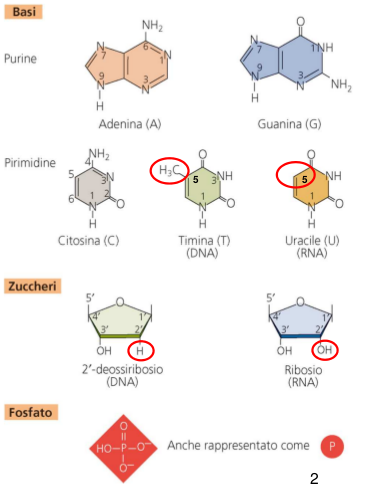
\includegraphics[scale=0.6]{img/01_Basi e zuccheri.png}
\caption{Basi e zuccheri degli acidi nucleici}
\label{Basi e zuccheri}
\end{figure}

Quando una delle suddette basi è legata alla posizione 1 di uno
zucchero, abbiamo i \textbf{nucleosidi}.

Ai nucleosidi possono essere legati da uno a tre gruppi fosfato e, in
tal caso, prendono il nome di \textbf{nucleotidi}.

Il gruppo fosfato conferisce una valenza acida alla molecola. Il gruppo
fosfato può trovarsi legato al carbonio 5' dello zucchero oppure al
carbonio 3'.

I nucleotidi che vengono utilizzati come substrato per la sintesi del
DNA e dell'RNA hanno 3 gruppi fosfato legati in serie sulla posizione 5'
dello zucchero.

Le basi possono subire modificazioni chimiche che sono essenziali per i
processi biologici che coinvolgono il DNA e gli RNAs.

Lo scheletro della catena polinucleotidica è costituito dall'alternanza
di zuccheri e di gruppi fosfato, mentre le basi azotate sporgono
lateralmente da questo scheletro. Ciascuna base è legata alla posizione
1' di uno zucchero da un legame glicosidico che interessa l'N1 delle
pirimidine o l'N9 delle purine. Tra uno zucchero e l'altro c'è un solo
gruppo fosfato e che quindi si tratta di un polimero di nucleosidi
monofosfato. Durante la sintesi degli acidi nucleici, ciascun nucleoside
trifosfato utilizzato come substrato, perde due dei suoi tre gruppi
fosfato. Ciascun gruppo fosfato forma un \textbf{legame estere} con il
C5' di uno zucchero e un secondo legame estere con il C3' dello zucchero
successivo. Questo tipo di legame, chiamato \textbf{fosfodiesterico},
conferisce una sorta di asimmetria (o polarità) alla catena, nel senso
che questa presenta due diverse estremità: da una parte c'è un
nucleotide che ha il C5' libero, mentre il C3' è impegnato nel legame
fosfodiesterico con il nucleotide adiacente; dall'altra la molecola
polimerica termina con un nucleotide che ha il C5' impegnato nel legame
fosfodiesterico con quello adiacente, mentre il C3' è libero. La loro
valenza è comunque impegnata da gruppi -OH o da gruppi fosfato.

\subsection{Struttura fisica del DNA}\label{struttura-fisica-del-dna}

Il DNA è formato da due catene polinucleotidiche antiparallele avvolte
l'una sull'altra a formare una struttura a doppia elica con lo scheletro
zucchero-fosfato posto sul lato esterno e le basi impilate all'interno.

Secondo il modello proposto da Watson e Crick le coppie di basi, che con
i loro anelli esterociclici sono strutture essenzialmente piatte, sono
disposte quasi perpendicolarmente rispetto all'asse della doppia elica.
Le basi basi che si affacciano in ciascuna coppia sono sempre una
pirimidina e una purina, ed è sempre presente l'appaiamento A-T/U o C-G
(questo giustifica la regolarità del diametro della doppia elica).

Le coppie A-T sono legate da 2 legami idrogeno, mentre le coppie G-C
sono legate da 3 legami idrogeno.

La doppia elica (duplex) del DNA ha una struttura regolare, destrorsa,
compie un giro completo ogni 34 A e ha un diametro di circa 20 A. La
distanza tra due coppie di basi adiacenti è di 3,4 A e ci sono, quindi,
circa 10,4 coppie di basi per ogni giro di elica. L'elica presenta
un'asimmetria dovuta alla posizione delle molecole di deossiribosio ai
lati delle basi: come conseguenza della opposta polarità
5'\(\rightarrow\) 3' delle due eliche, i due zuccheri di ciascuna coppia
di nucleotidi si vengono a trovare dallo stesso lato. Questa asimmetria
genera nella doppia elica due solchi di dimensioni diverse detti
\textbf{solco maggiore} e \textbf{solco minore}, con diametro 22 A e 12
A rispettivamente.

\subsubsection{Strutture alternative del
DNA}\label{strutture-alternative-del-dna}

La struttura del DNA proposta da Watson e Crick non è l'unica possibile.
Tale forma è detta \textbf{forma B} ed è stata ottenuta da studi di
diffrazione ai raggi X condotti in condizioni di \emph{alta umidità
(95\%)} e \emph{bassa salinità (condizioni cellulari)}.

Se si riduce l'umidità relativa in cui si trova la fibra di DNA, esso
assume la \textbf{forma A}. Questa forma è destrorsa come la B, ma se ne
differenzia per vari aspetti:

\begin{itemize}
\itemsep1pt\parskip0pt\parsep0pt
\item
  il passo dell'elica è di 25 A e il diametro di 23 A (è più tozza
  rispetto alla forma B);
\item
  presenta 11 coppie di basi per ogni giro dell'elica
\item
  le coppie di basi presentano una maggiore rispetto al piano
  perpendicolare all'asse della doppia elica;
\end{itemize}

Questa forma è stata riconosciuta tramite studi di diffrazione ai raggi
X in condizioni di \emph{minore umidità (75\%)} e \emph{alta salinità}.
Questa è, in vivo, la struttura tipica dei duplex DNA-RNA e RNA-RNA. Il
2'-OH del ribosio impedisce alla molecola di assumere la forma B.

L'ultima conformazione è la \textbf{forma Z}. Questa forma è
\emph{sinistrorsa} a causa del cambiamento dell'orientamento del legame
glucosidico base-zucchero tra la guanina e il deossiribosio. Nella forma
B lo zucchero e la base sono presenti nella conformazione ``anti'',
mentre nella forma Z si presentano nella conformazione ``syn''. La forma
Z ha un passo di 46 A, con 12 coppie di basi per giro d'elica, e un
diametro di 18 A. Rispetto alla forma B (passo 34Å), questo DNA ha una
forma allungata e magra.

Questa forma è stata riconosciuta tramite studi di diffrazione a raggi X
in condizioni di \emph{alta salinità} o in presenza di alcoli. Sono
state isolate proteine che legano ad alta affinità la forma Z e prove
sperimentali dicono che una piccola percentuale del DNA in vivo si trova
in questa forma.

Esistono altre forme che non analizzeremo (C,D e E).

\subsection{Topologia del DNA e DNA
topoisomerasi}\label{topologia-del-dna-e-dna-topoisomerasi}

La struttura di due filamenti avvolti in una doppia elica pone die seri
problemi durante i vari processi che richiedono un'apertura dell'elica e
la separazione dei due filamenti, dove il DNA si attorciglia us se
stesso a formare strutture complesse, dette \textbf{superavvolgimenti}.
Lo stato superavvolto del DNA contiene, come in una molla, l'energia che
viene utilizzata proprio per aprire i due filamenti Le molecole di DNA
possono essere circolari o lineari, in entrambi i casi possono
presentarsi dei superavvolgimenti.

Questi superavvolgimenti causano una variazione nella
\textbf{topologia}, ovvero della conformazione nello spazio, del DNA.

Il cambiamento della topologia del DNA è un aspetto fondamentale per
tutte quelle attività funzionali che richiedono una separazione dei
filamenti (replicazione, trascrizione, ricombinazione, ecc.). Le
molecole di DNA sia batteriche che eucariotiche sono \emph{superavvolte
negativamente}. La separazione dei due filamenti è maggiormente favorita
nel DNA superavvolto negativamente che nel DNA rilassato.

Le conseguenze del superavvolgimento cambiano a seconda del verso di
attorcigliamento. Se il superavvolgimento è \emph{negativo} il DNA si
avvolge in \emph{direzione opposta} rispetto a quella della doppia
elica. In questo modo diminuisce il n° di basi per giro elica.

Se il superavvolgimento é \emph{positivo} il DNA si avvolge nella
\emph{stessa direzione} della doppia elica aumenta. In questo modo il il
n° di basi per giro d'elica aumenta.

In entrambi i casi si crea tensione all'interno del DNA.

Consideriamo due filamenti circolari chiusi: il numeor di volte che un
filamento dovrebbe passsare attraverso l'altro in maniera che essi
possano essere cioketamente separati generando due circoli in maniera
che essi possano essere completamente separati generando due circoli a
singolo filamento, si chiama \textbf{numero di legame (Lk)}.

La \emph{frequenza} (quante volte un filamento si avvolge sull'altro) e
la posizione si entrambi nello spazio tridimensionale possono essere
descritte da due grandezze:

\begin{itemize}
\itemsep1pt\parskip0pt\parsep0pt
\item
  il \textbf{twist (Tw)}, rappresenta il numero di giri della doppia
  elica rispetto all'asse centrale (definisce il grado di avvolgimento
  della doppia elica). Questo è una proprietà intrinseca alla molecola
  ed consiste nel n° totale bp/ n° bp per giro d'elica (10,4 per il DNA
  in forma B);
\item
  il \textbf{writhe (Wr)}, rappresenta il numero di volte che l'asse
  centrale della doppia elica incontra se stesso.
\end{itemize}

La somma di queste due grandezze indica il numero di volte che un
filamento si avvolge sull'altro ed è il numero di legame. Lk può dunque
essere definito dalla seguente equazione:

\textbf{Lk = Tw + Wr}

Questa equazione descrive le possibili conformazoni che il DNA assume
nello spazio tridimensionale.

Per il DNA circolare chiuso o il DNA lineare con estremità fissate, Lk è
un valore costante e non può essere modificato da nessuna deformazione
che non comporti la rottura e la riunione di uno o entrambi filamenti.

Pertanto se Wr cambia a causa di un superavvolgimento positivo o
negativo, il Tw dovrà cambiare nella direzione opposta.

Se Lk = costante

\textbf{\(\Delta\)Tw = - \(\Delta\)Wr}

Molecole circolari covalentemente chiuse di uguale lunghezza (stessa
sequenza di basi) ma che differiscono solo per il numero di legame, sono
definite \textbf{topoisomeri}.

Consideriamo ora il caso di un DNA circolare completamente rilassato
(cccDNA): il suo numero di legame Lk sarà uguale al suo twist e il
writhe sarà 0. Definiamo in questo caso \textbf{Lk = Lk\(_0\)}. Se
vogliamo paragonare il grado di superelicità di due DNA che hanno la
stessa lunghezza, come due diversi topoisomeri, questa differenza è
definita da:

\textbf{\(\Delta\)Lk = Lk - Lk\(_0\)}

Se il \(\delta\)Lk di un cccDNA è diverso da 0, la molecola conterrà
della tensione e sarà superavvolta. Con Lk \textless{} Lk\(_0\) e
\(\Delta\)Lk \textless{} 0, il DNA è superavvolto negativamente, se Lk
\textgreater{} Lk\(_0\) e \(\Delta\)Lk \textgreater{} 0, allora il DNA è
superavvolto positivamente

Senza introduzione di tagli, essendo Lk costante, se si forza il DNA a
cambiare Wr, la molecola compenserà cambiando Tw e viceversa.

Per modificare Lk occorre rompere la doppia elica \emph{(nick)} e far
ruotare i due filamenti l'uno rispetto all'altro in modo da aumentare o
diminuire il numero di volte che un filamento si incrocia con l'altro.

\clearpage
\begin{figure}[htp]
\centering
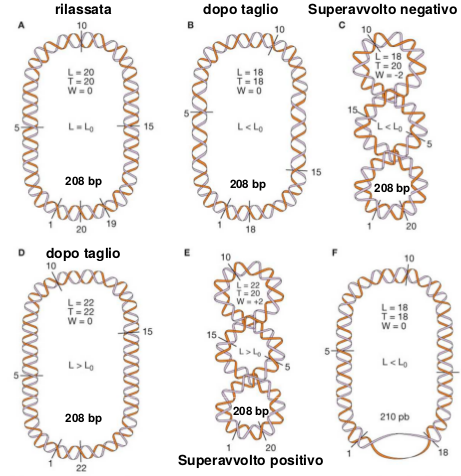
\includegraphics[scale=0.55]{img/02_Superavvolgimenti.png}
\caption{I superavvolgimenti}
\label{superavvolgimenti}
\end{figure}

\textbf{Confronto fig. A-B-C} Se si riduce L di 2 unità, la molecola
introduce 2 superavvolgimenti negativi (Wr = -2) per ripristinare il
valore di TW=20 (208/10,4). L \textless{} Lk 0

\textbf{Confronto fig. D-E-F} Se si aumenta L di 2 unità, la molecola
introduce 2 superavvolgimenti positivi (Wr= +2) per ripristinare il
valore di Tw=20 (208/10,4) L \textgreater{} Lk 0

\subsubsection{Le topoisomerasi}\label{le-topoisomerasi}

Lo stato topologico del DNA deve essere tneuto sotto controllo e per
fare questo la doppia elica deve essere aperta e richiusa
temporaneamente. Per catalizzare queste reazioni complesse gli organismi
contengono una classe di enzimi specializzati, chiamati \textbf{DNA
topoisomerasi}, che lavorano per mantenere adeguato il livello di
superavvolgimento del DNA.

Questi sono enzimi altamente conservati che convertono (isomerizzano) un
topoisomero in un altro modificandone il numero di legame Lk.

Questi enzimi catalizzano la rottura e la ri-unione dei filamenti di DNA
introducendo nick temporanei: creano un taglio transiente sul DNA
mediante una tirosina che si lega covalentemente allo scheletro fosfato,
con una reazione di transesterificazione fatta dal suo gruppo -OH. Dopo
la manipolazione topologica che aumenta o diminuisce Lk, il gruppo -OH
libero dle filamente tagliato, attraverso una reazione inversa, attacca
il legame tra la tirosina e il DNA, ripristinando la continuità della
doppia elica.

L'intero processo di modificazione topologica utilizza l'energia libera
contenuta nel DNA superavvolto senza richiesta di ATP aggiuntivo.

Le estremità del DNA generate dalla rottura del filamento non sono mai
libere, ma sono manipolate dentro i confini dell'enzima.

Alcune topoisomerasi possono rimuovere (e perciò rilassare)
superavvolgimenti negativi, altre sia positivi che negativi.

Le DNA topoisomerasi si differenziano tra loro per il meccanismo di
azione con il quale cambiano la topologia del DNA. Esistono due
principali strategie:

\begin{enumerate}
\def\labelenumi{\arabic{enumi}.}
\itemsep1pt\parskip0pt\parsep0pt
\item
  \textbf{rotazione controllata}, l'enzima introduce una singola rottura
  su un filamento della doppia elica e permette la rotazione su sé
  stesso del filamento intatto per un numero variabile di giri, fino a
  che l'attrito tra il DNA e l'enzima induce la rilegazione del
  filamento tagliato;
\item
  \textbf{strand passage}, consiste nel creare una rottura singola o a
  doppio filamento sul DNA, allargare l'interruzione prodotta e far
  passare l'altro filamento o la doppia elica attraverso la rottura che
  successivamente verrà risaldata.
\end{enumerate}

Le topoisomerasi vengono classificate sulla base della sequenza a.a.
osulla base del meccanismo di reazione.

In base al meccanismo di reazione si gli enzimi si suddividono in:

\begin{itemize}
\itemsep1pt\parskip0pt\parsep0pt
\item
  \textbf{topoisomerasi di tipo I}, sono in genere dei monomeri che
  tagliano un solo filamento del DNA al 5', creando in questo modo
  un'apertura mediata dalle interazioni di diversi domini dell'enzima
  con la doppia elica, attraverso la quale può passare l'altro filamento
  o una doppia elica. Questo meccanismo permette di eliminare con grande
  efficienza strutture annodate sul DNA e di rilassare esclusivamente
  superavvolgimenti negativi. Le topoisomerasi di tipo I, a seconda che
  formino un legame tirosina-5'fosfato o tirosina-3'fosfato, sono divise
  in \emph{tipo A} e \emph{tipo B} rispettivamente. Le tipo A richiedono
  anche ioni Mg\(^2\)\(^+\) o Zn\(^2\)\(^+\).
\end{itemize}

(immagine p41)

\begin{itemize}
\itemsep1pt\parskip0pt\parsep0pt
\item
  \textbf{topoisomerasi di tipo II}, sono in genere dei dimeri o
  multimetri che introducono un tagio su entrambi i filamenti del DNA
  con le due tirosine covalentemente legate all'estremità 5' e portano
  avanti le modificazioni topologiche facendo passare un secondo tratto
  a doppia elica attraverso la rottura. Il filamento tagliato si chiama
  segmento G (gate), il segmento che passa attraverso l'apertura si
  chiama segmento T (transport). Il meccanismo di azione della top II
  viene definito a \textbf{doppio cancello}. In questo processo il
  segmento T del DNA entra nella parte superiore dell'enzima, che si
  apre per accoglierlo; dopo l'apertura della doppia elica del segmento
  G, il segmento T attraversa tutto l'enzima, che si apre nella parte
  inferiore, rimuovendo in questa maniera due superavvolgimenti alla
  volta. Questo meccanismo richiede l'apporto di energia sotto forma di
  ATP per promuovere le modificazioni del complesso enzima-DNA (ma non
  per tagliare e risaldare i due filamenti). Queste topoisomerasi
  rilassano sia superavvolgimenti positivi che negativi.
\end{itemize}

\begin{figure}[htp]
\centering
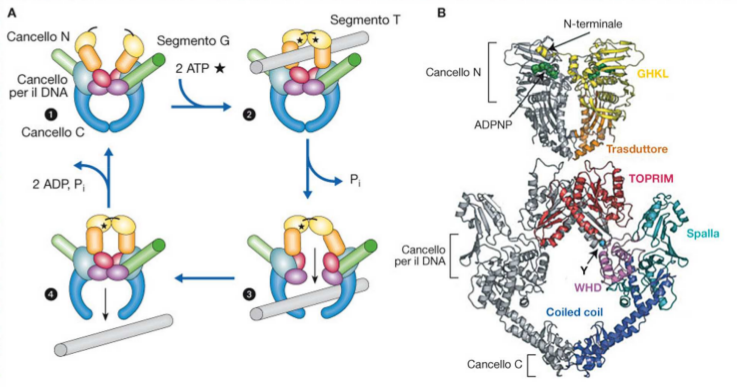
\includegraphics[scale=0.4]{img/03_Top II.png}
\caption{Topoisomerasi di tipo II}
\label{Top-II}
\end{figure}

In generale, le topoisomerasi sono coinvolte nei processi metabolici
associati alla separazione dei filamenti di DNA come la replicazione, la
trascrizione, la ricombinazione ed il riparo dell'acido nucleico. I due
filamenti del DNA, durante questi processi, devono essere separati
temporaneamente per diventare accessibili alle polimerasi o ai
componenti del complesso della trascrizione, di conseguenza il DNA
subisce degli stress torsionali che portano a dei superavvolgimenti
della molecola.

\textbf{Nomenclatura:} tutte le topoisomerasi di tipo I hanno un numero
dispari (I, III, V), mentre quelle di tipo II hanno un numero pari (II,
IV, VI). Le topoisomerasi con attività di superavvolgimento vengono
invece distinte in girasi (topoisomerasi di tipo II che introducono
superavvolgimenti negativi) e girasi inversa (topoisomerasi di tipo I
che introducono superavvolgimenti positivi).

La girasi di \emph{E. coli} è una topoisomerasi di tipo II ed è l'unica
in grado di introdurre superavvolgimenti negativi.

\section{La replicazione del DNA}\label{la-replicazione-del-dna}

Per trasmettere alle cellule figlie lo stesso patrimonio genetico della
cellula madre, l'informazione genetica contenuta nel DNA deve essere
duplicata con la massima fedeltà possibile, in quanto una variazione
nella sequenza nucleotidica genererebbe cambiamenti nel messaggio
genetico e dunque mutazioni.

Sulla base della struttura del DNA furono ipotizzati 3 possibili modelli
replicativi:

\begin{enumerate}
\def\labelenumi{\arabic{enumi}.}
\itemsep1pt\parskip0pt\parsep0pt
\item
  semiconservativo;
\item
  conservativo;
\item
  dispersivo.
\end{enumerate}

Il meccanismo di replicazione fu determinato nel 1958 da Meselson e
Stahl utilizzando la tecnica di \textbf{centrifugazione su gradiente di
densità}.

Inizialmente fecero crescere cellule di \emph{E. coli} in un terreno di
coltura a cui vennero aggiunti dei sali d'ammonio che contenevano
l'isotopo pesante dell'azoto \(^1\)\(^5\)N, al posto dell'isotopo
normale \(^1\)\(^4\)N. Le molecole di DNA che contengono \(^1\)\(^5\)N
hanno una ``densità'' maggiore rispetto a quella di molecole di DNA
contenenti \(^1\)\(^4\)N e, dopo centrifugazione all'equilibrio in
soluzioni concentrate di cloruro di cesio, si troveranno verso il fondo
della provetta da centrifugazione.

Le cellule di \emph{E. coli} vennero fatte duplicare per molte
generazioni in un terreno contenente sali pesanti dell'azoto, affinchè
tutte le cellule avessero molecole di DNA contenenti \(^1\)\(^5\)N. A
quel punto, le cellule furono raccolte tramite centrifugazione, lavate
per togliere ogni traccia di terreno contenente \(^1\)\(^5\)N, diluite
in un terreno contenente sali d'ammonio con l'isotopo leggero
\(^1\)\(^4\)N e fatte crescere in queste condizioni per due generazioni.

Se fosse stata vera l'ipotesi semiconservatica, dopo una generazione,
tutte le cellule di \emph{E. coli} che avevano replicato il loro DNA
avrebbero dovuto avere molecole di DNA contenente un filamento parentale
marcato con \(^1\)\(^5\)N e un filamento neosintetizzato marcato con
\(^1\)\(^4\)N. Tutte le molecole avrebbero dovuto avere, quindi, una
densità intermedia rispetto a quella di un DNA a doppia elica tutto
pesante o tutto leggero.

Se invece fosse risultata vera l'ipotesi conservativa della replicazione
del DNA i ricercatori si aspettavano che alla prima generazione metà del
DNA sarebbe stato pesante e metà leggero.

\begin{figure}[htp]
\centering
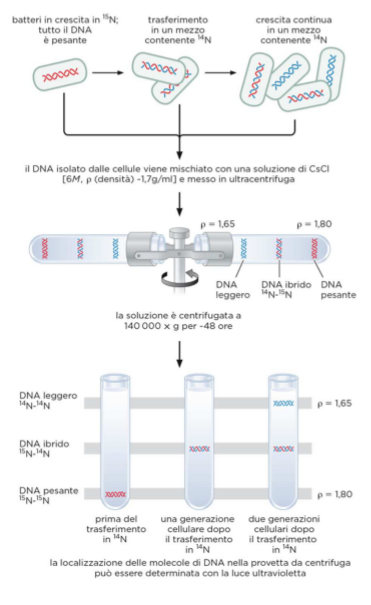
\includegraphics[scale=0.53]{img/05_Esperimento replicazione DNA.png}
\caption{Esperimento replicazione DNA}
\label{esperimento-replicazione-dna}
\end{figure}

\subsection{Il modello del replicone}\label{il-modello-del-replicone}

Un \textbf{replicone} è un'unità di DNA coinvolta nella replicazione.

Questo modello postula che l'inizio della replicazione del DNA è
geneticamente controllato da sequenze specifiche in \emph{cis} sul DNA
(chiamate \textbf{replicatori}). Queste sequenze determinano dove può
partire la replicazione del DNA interagendo con specifiche proteine
(\textbf{iniziatori}) che agiscono in \emph{trans} e collegano il
processo replicativo con la crescita e la divisione cellulare.

La replicazione del DNA necessita che i due filamenti si separino ed
inizia in punti specifici della molecola detti \textbf{origine di
replicazione}. La replicazione può essere \textbf{unidirezionale} o
\textbf{bidirezionale} a seconda del numero di forche replicative.

\emph{Unidirezionale} = una sola forca replicativa si allontana
dall'origine (rara, es. plasmide ColE1 di E. coli, fago \(\Phi\) 29 e
gli adenovirus). \emph{Bidirezionale} = due forche replicative procedono
contemporaneamente allontanandosi dall'origine in direzioni opposte.

\begin{figure}[htp]
\centering
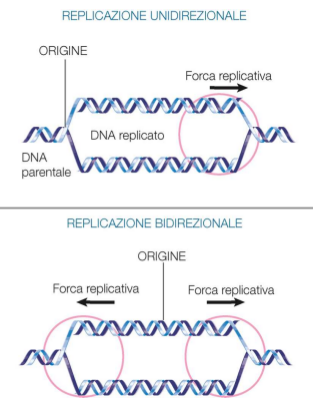
\includegraphics[scale=0.6]{img/06_Forche replicative.png}
\caption{Forche replicative}
\label{forche-replicative}
\end{figure}

Quando il DNA in replicazione viene osservato al microscopio elettronico
la regione replicata appare come una \textbf{bolla di replicazione}
all'interno del DNA non replicato. La bolla si estende fino a quando non
conterrà l'intero replicone

In tutti i cromosomi degli eucarioti esistono numerose origini di
replicazione. L'osservazione di ``bolle'' di replicazione di dimensioni
diverse indica due caratteristiche importanti delle origini dei
cromosomi degli eucarioti:

\begin{enumerate}
\def\labelenumi{\arabic{enumi}.}
\itemsep1pt\parskip0pt\parsep0pt
\item
  l'accensione delle origini non è simultanea, ma esistono delle origini
  ``early'' che vengono accese presto durante la fase di replicazione
  del DNA, mentre altre origini ``late'' vengono attivate a tempi
  successivi;
\item
  Le forcelle di replicazione che avanzano in direzioni opposte sul
  cromosoma possono fondersi tra di loro.
\end{enumerate}

\begin{figure}[htp]
\centering
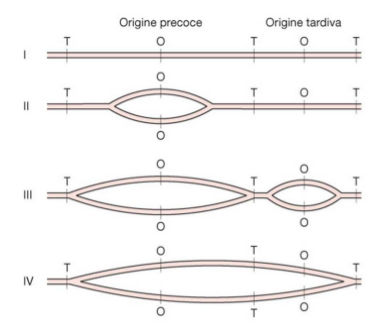
\includegraphics[scale=0.6]{img/07_Origini di replicazione.png}
\caption{Origini di replicazione}
\label{origini-di-replicazione}
\end{figure}

I repliconi batterici, come quello di \emph{E. coli}, sono normalmente
circolari e la replicazione procede in modo bidirezionale a partire da
una singola origine chiamata \emph{OriC}.

OriC di E. coli (genoma 4,2 Mbp) è una regione di 248 bp che contiene al
suo interno regioni che vengono riconosciute da proteine nelle fasi
iniziali della replicazione:

\begin{itemize}
\itemsep1pt\parskip0pt\parsep0pt
\item
  3 regioni di 13 bp ricche in AT;
\item
  4 regioni di 9 bp (siti di legame per l'iniziatore DnaA).
\end{itemize}

La particolarità di essere ricche in A e T è risultata, come vedremo,
una caratteristica comune alle origini di replicazione identificate in
altri organismi ed è legata al fatto che un'origine di replicazione, per
funzionare, deve potersi aprire ed è necessaria meno energia per
denaturare localmente una regione di DNA ricca in A e T piuttosto che in
C e G.

\subsection{Il processo replicativo}\label{il-processo-replicativo}

\subsubsection{La DNA polimerasi}\label{la-dna-polimerasi}

Il modello della replicazione semiconservativa del DNA suggerisce
immediatamente l'esistenza di enzimi in grado di catalizzare la
polimerizzazione dei nucleotidi. Se durante la replicazione ciascun
filamento serve da stampo per la neosintesi di un filamento
complementare, c'è da aspettarsi che nella cellula esistano delle
attività in grado di catalizzare la formazione del legame
fosfodiesterico tra nucleotidi in modo DNA stampo-dipendente. Tale
ipotesi portò all'identificazione della prima \textbf{DNA polimerasi}.

La sintesi del DNA ha delle precise richieste biochimiche: i substrati
della reazione sono i \textbf{deossiribonucleosidi trifosfati (dNTP)}, e
un \textbf{complesso innesco-stampo} costituito da uno stampo
rappresentato da un filamento di DNA e da un innesco che può essere un
tratto più o meno lungo di DNA che porti una estremità 3'OH che la DNA
polimerasi è in grado di allungare. Tutte le DNA polimerasi non sono in
grado di iniziare la sintesi della catena nucleotidica, ma necessitano
di una estremità 3'OH da allungare.

La DNA polimerasi aggiunge un nuovo nucleotide catalizzando la
formazione del legame fosfodiesterico nel rispetto della regola della
complementarietà tra le basi con il filamento di DNA stampo.

nella formazione di ciascun legame fosfodiesterico, il fosfato in
posizione \(\alpha\) del dNTP viene legato al 3'OH dell'innesco portando
alla liberazione di pirofosfato. L'energia libera di questa reazione è
piuttosto modesta, e l'energia addizionale che spinge la reazione verso
la polimerizzazione è fornita dall'idrolisi del pirofosfato da parte di
un enzima chiamato \textbf{pirofosfatasi}.

Le DNA polimerasi possiedono un'attività sintetica con polarità 5'
\(\rightarrow\) 3'.

\clearpage
\begin{figure}[htp]
\centering
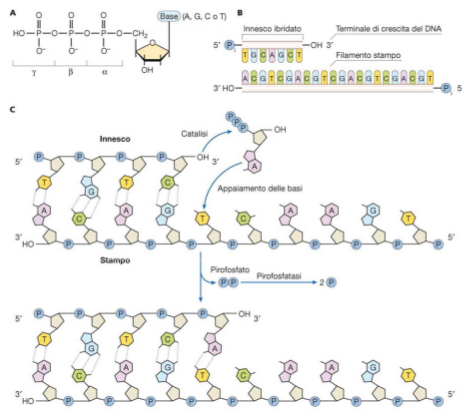
\includegraphics[scale=0.6]{img/08_DNA polimerasi.png}
\caption{}
\label{dna-polimerasi}
\end{figure}

La struttura delle DNA polimerasi replicative è paragonata a quella di
una mano parzialmente chiusa dove si distinguono 3 domini: pollice, dita
e palmo. Il DNA si lega ad una grande fessura compresa tra i 3 domini.
Il sito catalitico si trova nel palmo, mentre le dita sono coinvolte nel
posizionamento corretto dello stampo nel sito attivo. Il pollice lega il
DNA mentre esce dall'enzima ed è importante per la processività
dell'enzima. L'attività esonucleasica risiede in un dominio indipendente
con un proprio sito attivo.

\subsubsection{Fedeltà del processo
replicativo}\label{fedeltuxe0-del-processo-replicativo}

La fedeltà del processo replicativo è di circa 1 errore ogni
10\(^9\)-10\(^1\)\(^0\) nucleotidi polimerizzati.

Un sistema basato solo sulla stereochimica di coppie di basi che
rispettino la regola della complementarietà non sarebbe in grado di
raggiungere l'accuratezza indicata sopra. La selettività delle
polimerasi è piuttosto limitata (1 errore ogni 10\(^5\) circa) per la
presenza di forme tautomeriche delle basi azotate. Questi errori sono
rimosis da un'attività esonucleasica 3'\(\rightarrow\) 5' che ha,
quindi, una polarità invera alla direzione di sintesi del DNA. Tale
attività ha la funzione di agire come correttore di bozze
\textbf{(attività proofreading)}. Quando la DNA polimerasi rileva la
presenza di un appaiamento non corretto tra le coppie di basi, il
complesso stampo-innesco si allontana dal sito catalitico di
polimerizzazione della DNA polimerasi e si avvicina al sito
esonucleasico con funzione proofreading. Tale attività elimina il
nucleotide errato e permetta alla polimerasi di riprendere la sintesi
senza che il complesso ternario innesco-stampo-enzima si sia dissociato.

La fedeltà della replicazione del DNA può essere dunque riassunta in:

\begin{enumerate}
\def\labelenumi{\arabic{enumi}.}
\itemsep1pt\parskip0pt\parsep0pt
\item
  fedeltà;
\item
  attività di proofreadin;
\item
  riparazione degli errori.
\end{enumerate}

\subsubsection{Forcella di replicazione: sintesi del filamento continuo e
del filamento
discontinuo}\label{forcella-di-replicazione-sintesi-del-filamento-continuo-e-del-filamento-discontinuo}

Poichè tutte le DNA polimerasi possono polimerizzare il DNA soltanto in
direzione 5' \(\rightarrow\) 3', ciò crea un problema nella progressione
della forcella replicativa. Soltanto uno dei due filamenti di neosintesi
può essere sintetizzato in modo continuo seguendo la direzione della
forcella replicativa: questo filamento di neosintesi viene chiamato
\textbf{filamento continuo} o \textbf{leading strand}. Per rispettare la
polarità di sintesi del DNA (5' \(\rightarrow\) 3') l'altro filamento
deve essere sintetizzato in modo discontinuo e genera quello che viene
definito \textbf{filamento ritardato} o \textbf{lagging strand}. Tale
filamento è definito ritardato perchè la sua la sua sintesi può iniziare
solo dopo che il progredire della forcella di replicazione ha generato
sufficiente DNA a singolo filamento da far partire la sintesi del
filamento ``lagging''. La sintesi del filamento ritardato si realizza
attraverso la generazione di frammenti discontinui di DNA che vengono
chiamati \textbf{frammenti di Okazaki}.

\clearpage
\begin{figure}[htp]
\centering
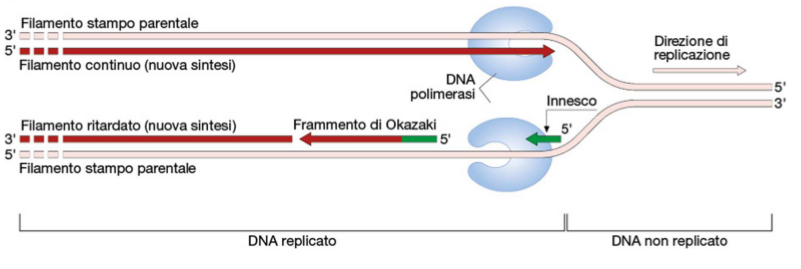
\includegraphics[scale=0.5]{img/12_Lagging-leading strand.png}
\caption{}
\label{lagging-leading-strand}
\end{figure}

La sintetizzazione discontinua del frammento lagging implica la
necessità di dell'enzima \textbf{DNA ligasi}, un enzima in grado di
saldare il 3'OH di un frammento di Okazaki con il 5'-fosfato del
frammento di Okazaki sintetizzato precedentemente.

\subsubsection{Innesco della sintesi di
DNA}\label{innesco-della-sintesi-di-dna}

L'innesco della sintesi di ogni frammento di Okazaki, così come
l'innesco del filamento a un'origine di replicazione, devono prevedere
la sintesi di un iniziatore (\emph{primer}) per offrire alla DNA
polimerasi il complesso stampo-iniziatore descritto poco sopra.
L'innesco della sintesi del DNA è fornito da corte (4-12 nucleotidi)
molecole di RNA sintetizzate da un enzima, denominato \textbf{DNA
primasi}.

\clearpage
\subsubsection{Le proteine replicative di E.
coli}\label{le-proteine-replicative-di-e.-coli}

\begin{figure}[htp]
\centering
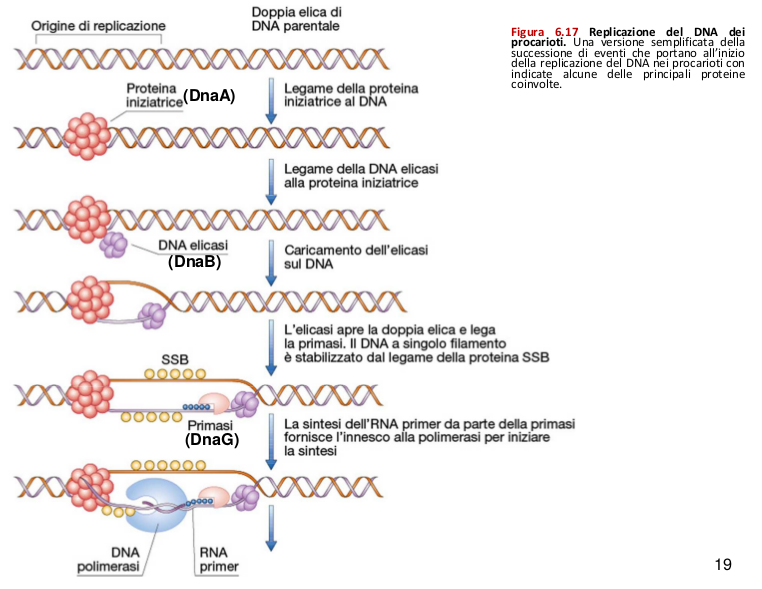
\includegraphics[scale=0.45]{img/09_Replicazione del DNA.png}
\caption{}
\label{replicazione-del-dna}
\end{figure}

Il primo evento molecolare consiste nel riconoscimento di \emph{ori C}
da parte della proteine \textbf{DnaA}. DnaA si attacca inizialmente alle
ripetizioni di 9 pb: la proteina si lega in modo cooperativo formando
una specie di nucleo centrale proteico intorno al quale si avvolge il
DNA di \emph{oriC}. Successivamente, DnaA si lega anche alle 3
ripetizioni di 13 pb facilitando la denaturazione localizzata del DNA in
quella regione e permettendo l'assemblaggio di altre proteine
replicative.

Il passaggio successivo consiste nel caricamento di \textbf{DnaB} e
\textbf{DnaC} a livello della bolla di denaturazione creatasi nella
regione di \emph{oriC} dando origine a un complesso proteico, denominato
\textbf{complesso di pre-innesco} della sintesi del DNA. DnaB possiede
un'attività elicasica, per cui consumando ATP è in grado di separare i
due filamenti di DNA. Lo svolgimento del DNA sia nella fase iniziale che
nel successivo processo di allungamento della sintesi del DNA genera una
tensione torsionale del DNA che è risolta da enzimi in grado di
modificare la topologia del DNA e chiamati ``DNA topoisomerasi''.

La bolla di denaturazione creatasi tende spontaneamente a rinaturare:
per evitare questo il DNA a singolo filamento originatosi viene
stabilizzato dal legame della \textbf{proteina SSB} alla regione di
ssDNA. SSB è una proteina che ha un'affinità maggiore per il DNA a
singolo filamento che a doppio filamento.

Le proteine DnaA e SSB interagiscono con il DNA in modo cooperativo:
questo sta a indicare che il legame tra una molecola di SSB all'ssDNA
facilita il legame di una seconda molecola di SSB alla stessa molecola
di DNA.

\begin{figure}[htp]
\centering
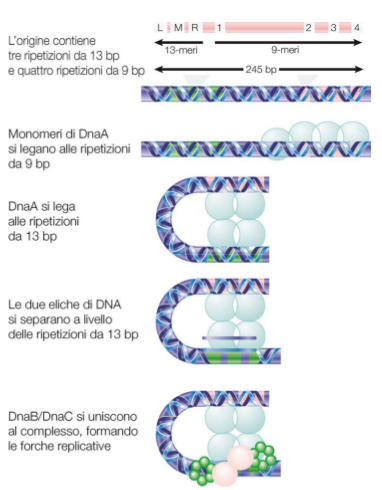
\includegraphics[scale=0.5]{img/10_Stadio pre-innesco.png}
\caption{}
\label{stadio-pre-innesco}
\end{figure}

Tutte le DNA polimerasi necessitano di un'estremità 3'OH pre-formata per
poter aggiungere i nucleotidi successivi. In E. coli e negli eucarioti,
però, gli inneschi che forniscono il 3'OH che può essere allungato dalla
DNA polimerasi sono corte molecole di RNA; tali molecole funzionano da
primer sia per far partire la sintesi continua a un'origine del
filamento leading, sia per iniziare la sintesi di tutti i grammenti di
Okazaki. La \textbf{DNA primasi} di E. coli, codificata dal \textbf{gene
dnaG}, è costituita da un singolo polipeptide e la sintesi degli
\textbf{RNA primer} costituisce il primo effettivo evento di sintesi
nella replicazione del DNA.

La DNA polimerasi replicativa di E. coli è la \textbf{DNA polimerasi III
oloenzima}, una macchina proteica molto complessa formata da numerose
subunità che si assemblano in modo sequenziale a formare un dimero
catalitico. Ci sono due copie del nucleo catalitico, che è formato da 3
subunità: \textbf{\(\alpha\)} (attività DNA polimerizzante),
\textbf{\(\varepsilon\)} (attività esonucleasica correttore di bozze
3'\(\rightarrow\) 5') e \textbf{\(\theta\)} (stimola la esonucleasi). Ci
sono anche due copie delle subunità \textbf{\(\tau\)}, che media la
dimerizzazione dei 2 nuclei catalitici. Questi possono assemblarsi sul
DNA solo dopo che un complesso di 5 proteine, chiamato
\textbf{``complesso \(\gamma\)''}, è riuscito a caricare sul DNA due
copie della subunità \(\beta\); per tale processo il complesso
\(\gamma\), che è una \emph{ATPasi DNA-dipendente}, richiede e consuma
ATP. La subunità \textbf{\(\beta\)} forma un omodimero con una forma a
ciambella in grado di abbracciare il singolo filamento di DNA che passa
nel foro della ciambella.

Il dimero \(\beta\) ha una struttura a forma di anello con un diametro
di 80 A ed una cavità di 35 A. Lo spazio tra l'anello proteico ed il DNA
è occupato da H\(_2\)O. L'anello \(\beta\) è legato al DNA, ma non entra
a contatto direttamente con il DNA; scivola sul DNA stabilendo o
eliminando contatti con le molecole di H\(_2\)O.

I due nuclei catalitici presenti nel modello dimerico di replicazione
del DNA replicano contemporaneamente il filamento leading e il filamento
lagging della doppia elica.

L'aspetto più importante del modello è che la sintesi del filamento
leading induce la formazione, sull'altro filamento, di un'ansa che
fornisce lo stampo per la sintesi del filamento ritardato.

(Figura 6.19, p 161)

Il replisoma consiste dunque di un \textbf{dimero asimmetrico} formato
da \textbf{2 nuclei catalitici} (DNA polimerasi III) e da proteine
associate necessarie per la dimerizzazione e la funzione catalitica
della polimerasi (900 kDa):

\begin{itemize}
\itemsep1pt\parskip0pt\parsep0pt
\item
  2 copie di \textbf{nuclei catalitici} (\(\alpha\), \(\varepsilon\),
  \(\theta\));
\item
  2 copie della proteina \(\tau\), responsabile della dimerizzazione;
\item
  2 copie dell'anello \textbf{``clamp'' (pinza)}, formato da un
  omodimero della subunità \(\beta\). Questo mantiene i nuclei
  catalitici sul filamento stampo, si lega al DNA ed è responsabile
  della processività della polimerasi;
\item
  1 complesso \(\gamma\) o \textbf{``clamp loader''} formato da 5
  proteine, carica l'anello \(\beta\) sul DNA.
\end{itemize}

Il clamp loader utilizza ATP per caricare l'anello \(\beta\) sul
complesso stampo-primer. A questo punto \(\beta\) cambia conformazione e
lega il nucleo polimerasico. Il dimero \(\tau\) lega il nucleo
polimerasico e svolge la funzione di dimerizzazione legando un secondo
nucleo polimerasico associato ad un altro anello \(\beta\). Ciascuno dei
complessi catalitici sintetizza 1 dei nuovi filamenti di DNA. Durante la
sintesi del filamento guida la polimerasi resta sempre associata allo
stampo, mentre durante la sintesi del filamento ritardato la polimerasi
si associa e si dissocia alla fine della sintesi di ciascun frammento di
Okazaki, per poi riassociarsi all'innesco sintetizzato dalla primasi
nella regione dell'ansa. Il ``clamp loader'' resta associato al nucleo
polimerasico che sintetizza il filamento ritardato.

\begin{figure}[htp]
\centering
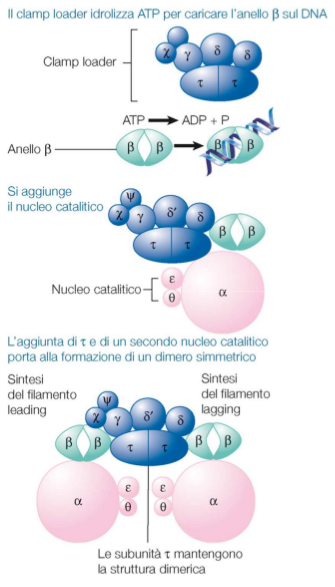
\includegraphics[scale=0.6]{img/11_Assemblaggio replisoma.png}
\caption{}
\label{assemblaggio-replisoma}
\end{figure}

\clearpage
Quando un frammento di Okazaki è completo l'anello \(\beta\) viene
aperto dal complesso \(\gamma\) rilasciando l'ansa. \(\gamma\) è una
pinza molecolare che tramite l'utilizzo di ATO riesce a modificare la
conformazione di \(\beta\). La polimerasi del filamento ritardato si
sposta da un anello \(\beta\) a quello successivo senza dissociarsi dal
complesso replicativo.

E. coli presenta dunque più DNA polimerasi:

\begin{itemize}
\itemsep1pt\parskip0pt\parsep0pt
\item
  \textbf{DNA polimerasi I} (103 kDa). Formata da un'unica subunità con
  due domini. Il frammento di Klenow (68 kDa) ha attività polimerasica
  ed esonucleasica 3' \(\rightarrow\) 5'. Il dominio con attività
  esonucleasica 5' \(\rightarrow\) 3' (35 kDa) rimuove i primer di RNA e
  poi riempie i vuoti tra i frammenti di Okazaki. Riempie anche i vuoti
  che si formano durante la riparazione del DNA. È l'unica con attività
  esonucleasica 5' \(\rightarrow\) 3';
\item
  \textbf{DNA polimerasi II}. Riempie le interruzioni in seguito a danno
  strutturale (risposta SOS inducibile);
\item
  \textbf{DNA polimerasi III}. È resposabile dell'allungamento della
  forcella di replicazione. Svolge polimerizzazione in direzione 5'
  \(\rightarrow\) 3' e attività esonucleasica in direzione 3'
  \(\rightarrow\) 5'. Possiede un nucleo catalitico formato da 3
  subunità \(\alpha\) (attività polimerasica), \(\varepsilon\)
  (esonucleasica 3' \(\rightarrow\) 5') e \(\theta\) (stimolo
  all'esonucleasi);
\item
  \textbf{DNA polimerasi IV e V}, sintesi di DNA translesione (bypass).
\end{itemize}

Nel DNA completamente replicato non possono venire inglobati i piccoli
frammenti di RNA sintetizzati dalla DNA primasi: questi vengono
principalmente rimossi dall'attività esonucleasica 5' \(\rightarrow\) 3'
della DNA polimerasi I che, mentre elimina gli RNA primer, è in grado di
riempire i buchi o ``gap'' che essa stessa genera. I ``nick'', cioè le
interruzioni che rimangono tra i vari frammenti di Okazaki sono, infine,
saldati dall'azione della \textbf{DNA ligasi} che unisce i frammenti
legando l'estremità 3'-OH di un frammento con il 5'-fosfato del
frammento seguente.

La reazione ligasica avviene in due stadi. Inizialmente l'enzima forma
un complesso con l'AMP e si lega al 5'-fosfato del DNA formando il
\emph{complesso ligasi-AMP-5'P-DNA}. Successivamente viene formato un
legame fosfodiestere tra il 3'-OH ed il complesso ligasi-AMP-5'P-DNA.
L'enzima di E. coli utilizza NAD come cofattore in sostituzione ad ATP,
mentre la ligasi 16 del fago T4 utilizza ATP.

\clearpage
\begin{figure}[htp]
\centering
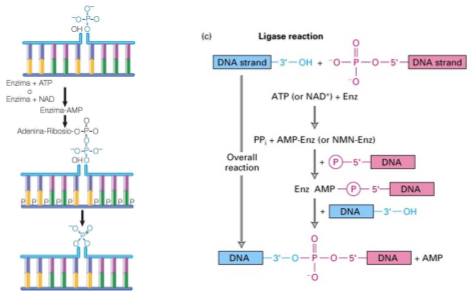
\includegraphics[scale=0.5]{img/13_Reazione ligasica.png}
\caption{}
\label{replicazione-ligasica}
\end{figure}

La terminazione della replicazione di E. coli è controllata da
ripetizioni di una breve sequenza di 23 pb, chiamata \textbf{ter}. Le
sequenze \emph{ter} sono posizionate a circa 180° rispetto a \emph{oriC}
e le diverse sequenze fanno terminare l'una o l'altra delle due forcelle
di replicazione. Per impedire il movimento delle forcelle di
replicazione le sequenze \emph{ter} vengono riconosciute da una
\textbf{controelicasi unidirezionale (Tus)} che lega una proteina
chiamata \textbf{TBP (Ter Binding Protein)} che impedisce alla forca
replicativa di procedere oltre.

Durante la terminazione della replicazione è anche necessaria l'azione
di DNA topoisomerasi per separare fisicamente le due molecole di DNA
circolari che si sono originate.

\subsection{Meccanismo di replicazione degli
eucarioti}\label{meccanismo-di-replicazione-degli-eucarioti}

Per molti aspetti la replicazione degli eucarioti è molto simile a
quella batterica (semiconservativa, bidirezionale e simidiscontinua).

Negli eucarioti, a causa della maggior quantità di DNA presente, le
origini di replicazioni sono numerose (+ repliconi).

Gli eucarioti presentano un maggior numero di DNA polimerasi. Le
sequenze delle origini di replicazione non sono ben definite a parte
quella del lievito S. cerevisiae (ARS).

La replicazione negli eucarioti avviene durante la fase S del ciclo
cellulare.

Il modello di studio di questo meccanismo è stato il virus delle scimmie
SV40 il quale utilizza per lo più l'apparato replicativo dell'ospite.

La velocità di replicazione negli eucarioti è di 500-3.500 basi/min,
mentre in E. coli è di 50.000 basi/min.

\subsubsection{Polimerasi eucariotiche}\label{polimerasi-eucariotiche}

Le DNA polimerasi degli eucarioti si dividono in:

\begin{itemize}
\itemsep1pt\parskip0pt\parsep0pt
\item
  \textbf{replicative}, sono enzimi multimerici. Possiedono una subunità
  responsabile della catalisi e una subunità con funzioni ausiliarie
  (es. sintesi dell'innesco, processività\ldots{}). Replicano il DNA con
  alta fedeltà.
\item
  \textbf{riparative}, sono più semplici. Generalmente sono formate da
  una subunità e distinte in polimerasi riparative ad alta fedeltà e
  polimerasi inclini all'errore (sintesi di translesione).
\end{itemize}

Nella replicazione del DNA nucleare eucariote sono coinvolte 3
polimerasi:

\begin{enumerate}
\def\labelenumi{\arabic{enumi}.}
\itemsep1pt\parskip0pt\parsep0pt
\item
  \textbf{polimerasi \(\alpha\)} (inizia la sintesi dei nuovi
  filamenti);
\item
  \textbf{polimerasi \(\varepsilon\)} (allunga il filamento continuo);
\item
  \textbf{polimerasi \(\delta\)} (allunga il filamento discontinuo).
\end{enumerate}

La polimerasi \(\alpha\) è atipica. Questa polimerasi è capace di
iniziare la sintesi di una nuova catena e può iniziare sia la sintesi
del filamento continuo che di quello ritardato. La pol \(\alpha\) è
formata da più subunità: una subunità catalitica (180 kDa) e tre
subunità accessorie. Le subunità accessorie sono formate da una subunità
B, necessaria per l'assemblaggio del complesso, ed altre due subunità
più piccole per l'attività primasica (RNA polimerasi). Il complesso è
chiamato \textbf{polimerasi \(\alpha\)-primasi}.

\subsubsection{Il processo replicativo negli
eucarioti}\label{il-processo-replicativo-negli-eucarioti}

Per dividersi e proliferare, tutte le cellule eucariotiche devono
eseguire correttamene un programma genetico, definito ciclo cellulare,
che sovrintende alla corretta replicazione e segregazione del materiale
ereditario nelle cellule figlie.

La selezione e preparazione delle origini di replicazione del DNA negli
eucarioti inizia quando le cellule escono dalla mitosi e prosegue nella
fase G1 del ciclo cellulare. In questo lasso di tempo si forma su
ciascuna origine un \textbf{complesso di pre-replicazione (pre-RC)}.

Il costituente principale del pre-RC è il complesso ORC. Il complesso
pre-RC comincia a formarsi quando al complesso ORC si agganciano due
proteine chiamate \textbf{Cdc6} e \textbf{Cdt1}; queste sono richieste
per il caricamento del complesso dell'elicasi, nota come
\textbf{MCM2-7}. L'attività delle proteine chinasi CDK trasforma il
pre-RC in quello che è chiamato \textbf{pre-initiation complex}, cioè
una macchina proteica più complessa che diventa competente per la
replicazione e innesca la sintesi vera e propria del DNA. Eventi di
fosforilazione catalizzati dalle CDK provocano il distacco di Cdc6 e
Cdt1, e il contemporaneo aggancio di altre proteine.

\begin{figure}[htp]
\centering
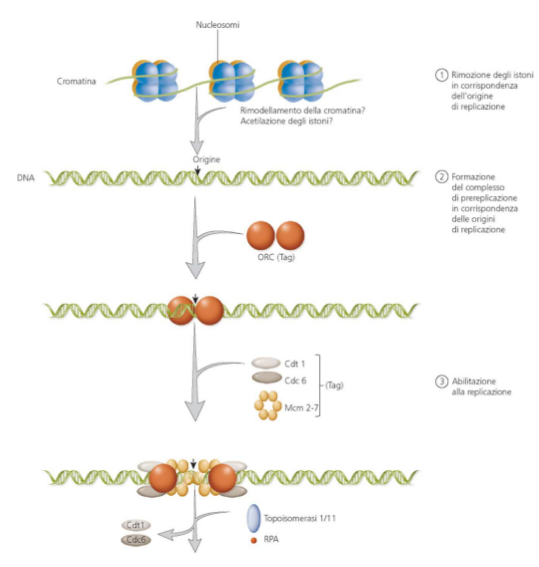
\includegraphics[scale=0.6]{img/16_complesso pre-replicazione.png}
\caption{}
\label{complesso-pre-replicazione}
\end{figure}

Durante la fase S viene attivata l'elicasi. In questo processo sono
coinvolte 2 proteine chinasi, \textbf{CDK (ciclin dependent kinase)} e
\textbf{DDK (Dbf4, dependent kinase)}, inattive durante la fase G1. CDK
attiva \textbf{Sld2} e \textbf{Sld3}, mentre DDK attiva Mcm2-7.

Sld2 e Sld3, quando vengono fosforilate, legano \textbf{Dpb11} ed
insieme facilitano il legame di \textbf{GINS} e \textbf{Cdc45}
all'elicasi.

\begin{figure}[htp]
\centering
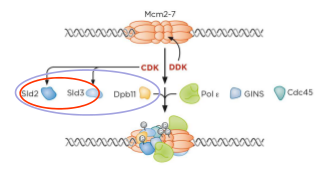
\includegraphics[scale=0.8]{img/14_Complesso replicazione01.png}
\caption{}
\label{complesso-replicazione01}
\end{figure}

Nella \emph{fase G1} Mcm2-7, non attiva, viene caricata intorno al dsDNA
come dimero (2 elicasi). Nella \emph{fase S}, dopo il legame di Cdc45 e
GINS, un filamento di DNA viene espulso dal canale centrale di ciascuna
elicasi. Le interazioni tra le due elicasi vengono eliminate.

\begin{figure}[htp]
\centering
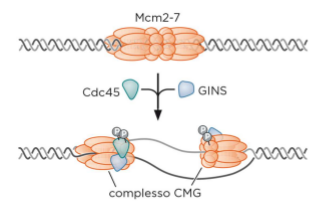
\includegraphics[scale=0.6]{img/15_Complesso replicazione02.png}
\caption{}
\label{complesso-replicazione02}
\end{figure}

L'inizio della sintesi di DNA sulla leading strand richiede l'azione del
\textbf{complesso DNA polimerasi \(\alpha\)-primasi} che porta alla
sintesi del primo RNA primer (circa 10 bp) e 20-30 basi di DNA (iDNA =
iniziatore).

A questo stadio avviene una reazione definita \textbf{scambio delle
polimerasi}. Pol \(\alpha\)-primasi viene sostituita dalla DNA
polimerasi \(\delta\) sul 3'OH della catena nascente di DNA. Per
effettuare questo scambio intervengono due proteine proteine:

\begin{itemize}
\itemsep1pt\parskip0pt\parsep0pt
\item
  \textbf{PCNA},un trimero, simile all'anello \(\beta\) di E. coli;
\item
  \textbf{RFC} (simile al clamp loader \(\gamma\) di E. coli).
\end{itemize}

La pinza PCNA viene caricata sul DNA per azione di RFC, il quale
utilizza ATP per aprire l'anello PCNA.

Pol \(\alpha\)-primasi viene rimpiazzata da pol \(\delta\) sul filamento
lento e pol \(\varepsilon\) sul filamento guida.

Nella sintesi del DNA degli eucarioti la processività della pol
\(\delta\) e \(\varepsilon\) dipende da PCNA, mentre nei procarioti
dipende dall'anello \(\beta\).

\begin{figure}[htp]
\centering
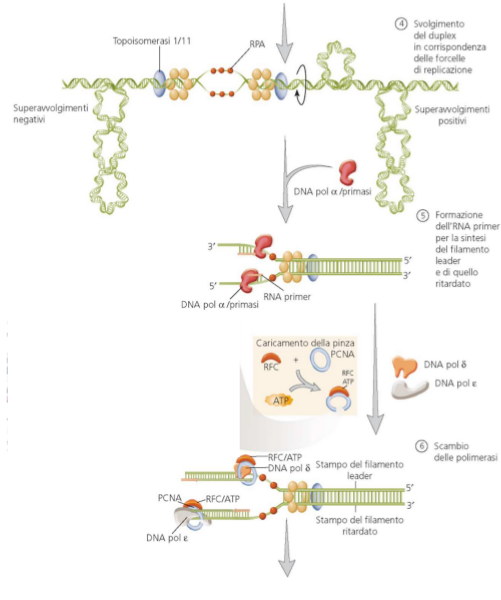
\includegraphics[scale=0.7]{img/17_Scambio delle polimerasi.png}
\caption{}
\label{scambio-delle-polimerasi}
\end{figure}

\clearpage
Successivamente interviene \textbf{FEN1}, una esonucleasi, a rimuovere i
primer di RNA e, formando un complesso con DNA polimerasi \(\delta\)
sintetizza DNA in modo analogo alla DNA pol I di E. coli.

\begin{figure}[htp]
\centering
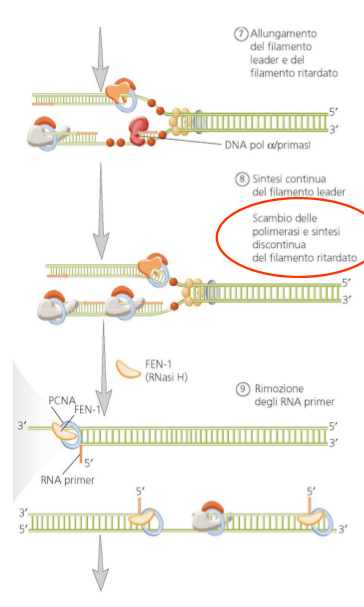
\includegraphics[scale=0.5]{img/18_FEN1.png}
\caption{}
\label{fen1}
\end{figure}

\clearpage
Infine interviene una ligasi che lega i frammenti mediante la formazione
di un legame fosfodiestere.

\begin{figure}[htp]
\centering
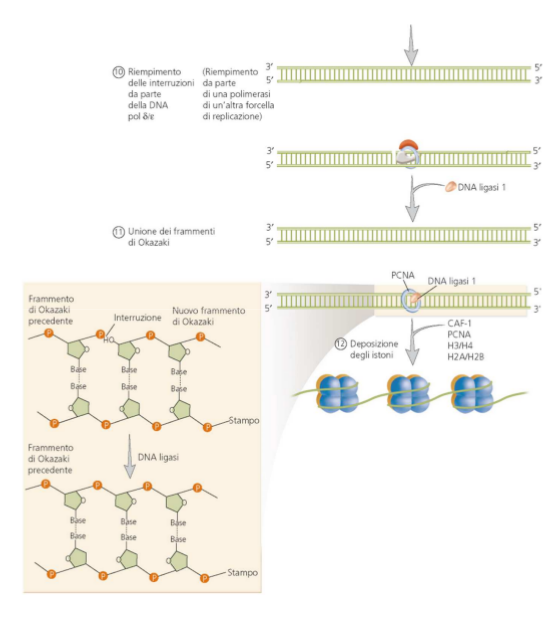
\includegraphics[scale=0.5]{img/19_ligasi.png}
\caption{}
\label{ligasi}
\end{figure}

Non è noto un equivalente di \(\tau\) di E. coli responsabile della
coordinazione della replicazione negli eucarioti.

Una differenza tra procarioti ed eucarioti è che nei procarioti, non
appena vengono reclutate le proteine iniziatrici in corrispondenza delle
origini, vengono reclutate anche le DNA elicasi e la sintesi inizia.

Nelle cellule eucariote invece, si ha la formazione di un complesso di
pre-replicazione (abilitazione alla replicazione) che avviene in un
altro momento del ciclo (Fase G1). Una volta che la cromatina eucariota
è stata aperta, le proteine iniziatrici riconoscono la sequenza di DNA
all'origine e vi si legano formando il complesso ORC-Cdc6-Cdt1 che,
idrolizzando ATP, carica l'elicasi Mcm2-7. Quando Mcm2-7 è caricato, il
complesso Cdc6-Cdt1 non serve più. Solo quando la cellula entra nella
fase S, l'elicasi si attiva e viene caricata la pol \(\alpha\)-primasi
ed inizia la sintesi.

Gli eventi di abilitazione alla replicazione sono sotto il controllo
dell'attività CDK/ciclina. La formazione del complesso di
pre-replicazione avviene solo quando l'attività CDK è bassa, nella fase
G1 del ciclo. In questa fase si forma il complesso ORC-Cdc6-Cdt1 e viene
caricato Mcm2-7.

\subsection{La replicazione dei
telomeri}\label{la-replicazione-dei-telomeri}

Nei cromosomi eucarioti lineari è sorto un problema legato al meccanismo
di sintesi discontinua del filamento lagging. Mentre la replicazione del
filamento leading continua fino a copiare l'estremità 5', nella
replicazione del filamento lagging rimane il tratto dell'RNA primer 5'
che, una volta rimosso, lascia un segmento di DNA non replicato che non
può essere riempito da alcuna delle polimerasi conosciute.

Le regioni terminali dei cromosomi eucariotici sono note come
\textbf{telomeri} e la loro struttura è molto importante per il
controllo della stabilità del genoma. I telomeri sono strutture
specializzate per proteggere le estremità dei cromosomi lineari.

I telomeri sono costituiti da sequenze di DNA contenenti numerose
ripetizioni in tandem di brevi sequenze ricche in G che lasciano
un'estremità sporgente in 3' (nell'uomo è 5'-TTAGGG-3').

I telomeri hanno una struttura ripetitiva con un filamento ricco in G-T
che si allunga oltre un filamento ricco in C-A. L'estensione G-T rimane
a singolo filamento per 14-16 basi ed è probabilmente prodotta da una
degradazione specificatamente limitata al filamento ricco in C-A.

Il numero di ripetizioni è variabile nelle diverse specie: nell'uomo
sono lunghe 5-10 kbp, mentre nel lievito 300 bp.

I telomeri svolgono 3 funzioni:

\begin{enumerate}
\def\labelenumi{\arabic{enumi}.}
\itemsep1pt\parskip0pt\parsep0pt
\item
  proteggono le estremità del cromosoma;
\item
  permettono al telomero di essere esteso;
\item
  facilitano la riorganizzazione dei cromosomi meiotici.
\end{enumerate}

Legate ai telomeri vi sono anche due proteine, \textbf{TRF1} e
\textbf{TRF2} (nei mammiferi), che riconoscono e legano la sequenza
telomerica, proteggendo così le estremità del DNA.

È stato osservato che le estremità dei telomeri non sono lineari, ma
assumono una struttura a forma di loop denominata \textbf{T-loop}.
Questa struttura è dovuta all'appaiamento tra le sequenze TTAGGG
dell'estremità 3' che protrude a singolo filamento e il filamento
complementare in un breve tratto denaturato nella ripetitiva adiacente
al duplex. La struttura è stabilizzata dalla formazione di complessi con
numerose proteine implicate nella funzione telomerica e nella protezione
dell'estremità del cromosoma.

Nei mammiferi le proteine sono 6: TRF1, TRF2, hRap1, TIN2, TPP1 e POT1.
Queste formano un complesso detto Schelterina che protegge i telomeri
dall'attività dei sistemi di riparo del danno al DNA.

Il mantenimento dei telomeri è assicurato dall'azione di un particolare
enzima, chiamato \textbf{telomeasi}. La telomerasi è una
ribonucleoproteina costituita da due componenti principali:

\begin{itemize}
\itemsep1pt\parskip0pt\parsep0pt
\item
  una proteina chiamata \textbf{TERT} che agisce come una trascrittasi
  inversa, essendo capace di sintetizzare DNA copiando uno stampo di
  RNA;
\item
  una molecola di RNA stampo, chiamata \textbf{TERC}.
\end{itemize}

La subunità catalitica TERT si associa con altre proteine accessorie
(chiamate Est) a formare la macchina proteica coinvolta nel mantenimento
dei telomeri.

Contrariamente a quanto ci si potrebbe aspettare, la telomerasi non
estende il filamento 5' ritardato più corto ma allunga ulteriormente il
terminale 3' sporgente. Per fare questo il terminale sporgente 3' si
appaia con il TERC della telomerasi, che ha una sequenza complementare
alla sequenza sporgente telomerica: la parte proteica della telomerasi
copia la sequenza del suo RNA allungando di una ripetizione la sequenza
3' sporgente. La successiva traslocazione e il riposizionamente della
telomerasi fanno sì che questo processo possa ripetersi più volte.

L'estensione delle sequenze ripetute da parte della telomerasi permette
di raggiungere un'omeostasi della lunghezza dei telomeri che non ne
altera la funzionalità e impedisce l'erosione dell'informazione
genetica.

Il numero di ripetizioni aggiunte è controllato da proteine ausiliarie
che funzionano come deboli inibitori ed impediscono alla telomerasi di
legare il DNA.

\section{Sistemi di riparazione del
DNA}\label{sistemi-di-riparazione-del-dna}

Variazioni nella sequenza nucleotidica del DNA prendono il nome di
\textbf{mutazioni}. Le mutazioni possono essere \emph{spontanee} (o
naturali) o \emph{indotte}, se dovute ad agenti mutageni esterni.

La maggior parte delle mutazioni sono definite \textbf{puntiformi}, in
quanto determinano il cambiamento di un singolo nucleotide. Le mutazioni
puntiformi sono divise in due categorie:

\begin{enumerate}
\def\labelenumi{\arabic{enumi}.}
\itemsep1pt\parskip0pt\parsep0pt
\item
  le \textbf{transizioni}, che sono cambiamenti da una purina a un'altra
  o da una pirimidina a un'altra;
\item
  le \textbf{trasversioni}, che sono cambiamenti da purina a pirimidina
  o da pirimidina a purina.
\end{enumerate}

Se durante il processo replicativo si introduce un appaiamento non
corretto tra i due filamenti del DNA e tale errore non viene riparato,
al secondo ciclo di replicazione del DNA la mutazione viene fissata nel
genoma.

Se il cambiamento nucleotidico cade nella regione di un gene codificante
per una proteina ci sono tre possibilità:

\begin{enumerate}
\def\labelenumi{\arabic{enumi}.}
\itemsep1pt\parskip0pt\parsep0pt
\item
  mutazione \textbf{silente (o sinonima)}, se la mutazione cambia la
  sequenza di una tripletta (codone) codificante per un certo
  amminoacido ma, grazie alla degenerazione del codice genetico, il
  nuovo codone codifica per lo stesso aa codificato dal codone
  originario;
\item
  mutazione \textbf{missenso}, se la mutazione puntiforme causa la
  formazione di un codone con un significato diverso dall'originario con
  conseguente cambiamento di un singolo aa. Questa mutazione può
  alterare le proprietà della proteina determinando una variazione nel
  fenotipo;
\item
  mutazioni \textbf{non senso}, se la sotituzione di un singolo
  nucleotide nella regione codificante di un gene determina la formazine
  di una delle 3 triplette non senso del codice genetico. Questo causa
  la formazione di una proteina tronca.
\end{enumerate}

Nel DNA possono verificarsi anche delle \textbf{delezioni} o
\textbf{inserzioni} di un singolo nucleotide. Questa perdita o aggiunta
di un nucleotide determina uno sfasamento del codice di lettura di un
gene codificante per una proteina. Queste mutazioni vengono chiamate
\textbf{frameshift} e alterano tutta la sequenza di amminoacidi a valle
del punto in cui è avvenuta la mutazione.

Alcune regioni del DNA hanno un'aumentata instabilità genomica a causa
della ripetizione di sequenze nucleotidiche. Se una sequenza di pochi
nucleotidi si ripete più volte in una regione di DNA, durante il
processo replciativo, le sequenze ripetute possono formare appaiamenti
strutturali alternativi con una stabilità termodinamica simile a quella
dell'appaiamento corretto. Le polimerasi possono, quindi, ``scivolare''
durante la replicazione di queste regioni, portando a una contrazione o
a un'espansione delle sequenze ripetute stesse.

Le mutazioni che causano un cambiamento del fenotipo possono essere
divise in due categorie: 1. la perdita di funzione o \textbf{loss of
function} è la conseguenza di una mutazione che abolisce o riduce
l'attività di una proteina; 2. l'acquisizione di funzione o \textbf{gain
of function} si verifica se la mutazione è in grado di conferire alla
proteina alterata codificata dal gene mutato una funzione anomala.

Le cause delle mutazioni possono essere:

\begin{itemize}
\itemsep1pt\parskip0pt\parsep0pt
\item
  errori di replicazione;
\item
  danni chimici e fisici come perdita o alterazione di basi, rottura
  dello scheletro, ecc.;
\item
  inserimento di trasposoni.
\end{itemize}

I danni causati al DNA possono essere dovuti a:

\begin{itemize}
\itemsep1pt\parskip0pt\parsep0pt
\item
  cambiamento di basi singole;
\item
  distorsioni strutturali (da raggi UV, agenti intercalanti, ecc);
\item
  danno all'ossatura del DNA (da siti abasici e da rotture del doppio
  filamento).
\end{itemize}

I processi riparativi possono essere raggruppati essenzialmente in 3
classi:

\begin{itemize}
\itemsep1pt\parskip0pt\parsep0pt
\item
  riparazione diretta del danno, in cui le basi vengono revertite
  chimicamente (es. fotoattivazione);
\item
  riparazione tramite escissione, in cui segmenti più o meno lunghi di
  un filamento di DNA danneggiato vengono eliminati con siccessiva
  sintesi riparativa utilizzando il filamento intatto come stampo;
\item
  riparazione tramite aggiramento del danno (sintesi di translesione).
\end{itemize}

Una prima opera di riparazione dei danni al DNA viene eseguita dalle DNA
polimerasi.

La \textbf{DNA polimerasi III}: questo complesso svolge, grazie alla
subunità \(\varepsilon\), un'attività esonucleasica 3' \(\rightarrow\)
5'.

L'inserimento di un nucleotide non corretto produce una deformazione
strutturale del filamento di DNA che induce la polimerasi a fermarsi o a
rallentare. Successivamente l'enzima retrocede e rimuove l'errore.

La \textbf{DNA polimerasi I} invece, svolge una funzione
\emph{``proofreading''}. questo enzima consiste di un'unic acatena
polipeptidica (103 kDa) che, mediante trattamento proteolitico può
essere suddivisa in due frammenti:

\begin{itemize}
\itemsep1pt\parskip0pt\parsep0pt
\item
  il maggiore, chiamato \textbf{frammento di Klenow} è dotato di
  un'attività polimerasica 5' \(\rightarrow\) 3' e di un'attività
  esonucleasica 3' \(\rightarrow\) 5' (correzione delle bozze). I due
  siti attivi sono separati 30 A (separazione spaziale tra il sito dove
  viene aggiunta la base da quello dove viene escissa);
\item
  il minore possiede anche un'attività esonucleasica 5' \(\rightarrow\)
  3', che determina l'escissione di nucleotidi a valle dell'enzima.
\end{itemize}

\subsection{Aggiramento della lesione: sintesi di
translesione}\label{aggiramento-della-lesione-sintesi-di-translesione}

La replicazione del DNA si blocca se trova una lesione (e.g.~dimeri di
T). La Pol III a questo punto si distacca e al suo posto entra la DNA
pol translesione. Copia il DNA con poca fedeltà, e poi si stacca per far
posto alla Pol III.

\begin{figure}[htp]
\centering
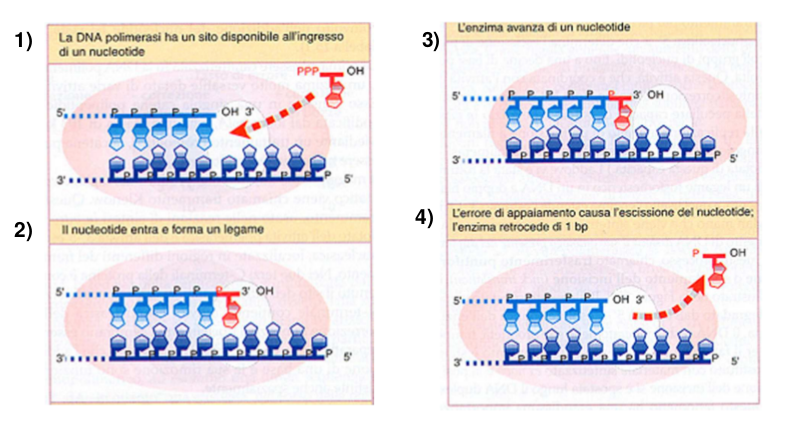
\includegraphics[scale=0.37]{img/21_DNA pol III.png}
\caption{}
\label{dna-pol-iii}
\end{figure}

\clearpage
Le DNA pol inclini all'errore si sostituiscono alla replicativa e
sintetizzano il tratto di DNA utilizzando le stesse proteine ausiliarie
(sintesi di translesione).

Aggirato il danno la pol viene sostituita nuovamente dalla pol
replicativa.

Queste polimerasi introducono errori con una frequenza 10\(^-\)\(^1\),
10\(^-\)\(^3\), ma risolvono il grave problema dell'arresto della
sintesi.

Le pol translesione in E. coli sono la DNA pol IV (dinB) e V (umuCD).

La sintesi delle DNA pol translesione è indotta in risposta al danno al
DNA. In E. coli RecA attiva DNA pol V umuD\(_2\)C a UmuD'\(_2\)C (è il
sistema SOS, vedi dopo).

\begin{figure}[htp]
\centering
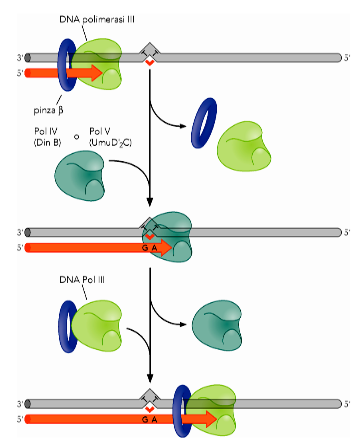
\includegraphics[scale=0.7]{img/22_Pol translesione.png}
\caption{}
\label{pol-translesione}
\end{figure}

\subsection{Reversione tramite
fotoliasi}\label{reversione-tramite-fotoliasi}

La fotoliasi è un enzima, appartenente alla classe delle liasi, che lega
specificamente i filamenti di DNA danneggiati dall'esposizione a
radiazione ultravioletta, le quali provocano la formazione di
\emph{dimeri di pirimidina} e di 6-4 fotoprodotti.

I dimeri di pirimidina si producono quando due basi azotate adiacenti
(timina e\o citosina) sullo stesso filamento di DNA vengono legate
covalentemente fra di loro. La fotoliasi ha alta affinità per queste
strutture chimiche, alle quali si lega reversibilmente e le ripara.

Questo enzima funziona come un meccanismo di riparazione del DNA quando
la luce di lunghezza d'onda compresa fra 320 e 370 nm lo colpisce
attivandolo. La reazione enzimatica prevede la rottura del dimero e la
ricostituzione della struttura corretta delle basi (fotoriattivazione).

Questo enzima è una flavoproteina che contiene due gruppi cromofori ed
agisce attraverso il trasferimento di elettroni. Nella reazione redox la
molecola FAD agisce da donatore di elettroni, mentre il dimero agisce da
accettore di elettroni.

La fotoliasi è presente e funzionante nei procarioti, è presente negli
eucarioti inferiori come il lievito dove si ritiene abbia però un ruolo
minore, ed è assente nelle cellule umane e nei mammiferi placentati in
genere.

\begin{figure}[htp]
\centering
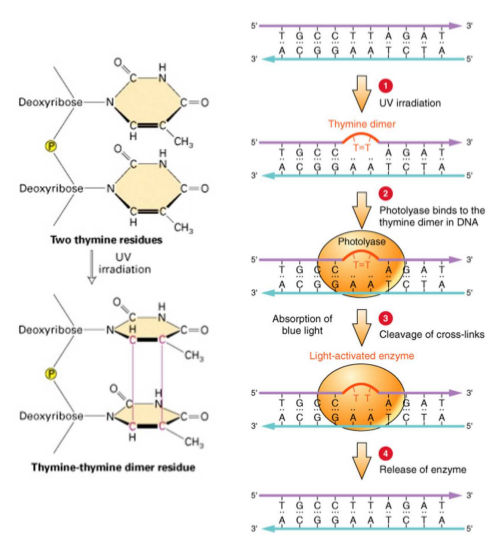
\includegraphics[scale=0.34]{img/23_Fotoliasi.png}
\caption{}
\label{fotoliasi}
\end{figure}

\clearpage
\subsection{Riparazione per
escissione}\label{riparazione-per-escissione}

I meccanismi di escissione possono essere di due tipi:

\begin{enumerate}
\def\labelenumi{\arabic{enumi}.}
\itemsep1pt\parskip0pt\parsep0pt
\item
  sistemi per \textbf{escissione di nucleotidi (NER)};
\item
  sistemi per \textbf{escissione delle basi (BER)}.
\end{enumerate}

Questi due sistemi condividono le stesse fasi del meccanismo:

\begin{enumerate}
\def\labelenumi{\arabic{enumi}.}
\itemsep1pt\parskip0pt\parsep0pt
\item
  Riconoscimento;
\item
  incisione (una endonucleasi taglia il filamento su entrambi i lati del
  danno);
\item
  rimozione (un'esonucleasi rimuove il DNA);
\item
  sintesi;
\item
  unione.
\end{enumerate}

\subsubsection{Sistemi NER in E. coli}\label{sistemi-ner-in-e.-coli}

Questo sistema si basa su diverse proteine chiamate globalmente
\textbf{Uvr} (UvrA, UvrB, UvrC e UvrD).

UvrA-UvrB cercano e riconoscono le distorsioni del DNA.

UvrB fonde (?) il DNA e recluta UvrC (UvrA viene rilasciato) che taglia
il DNA 8 nucleotidi a monte e 3-4 nucleotidi a valle del sito
danneggiato.

L'elicasi UvrD svolge la regione in cui è avvenuto il taglio permettendo
il rilascio del filamento tagliato.

Successivamente intervengono DNA Pol I per sintetizzare nuovamente la
porzione di DNA tagliata e ligasi.

\clearpage
\begin{figure}[htp]
\centering
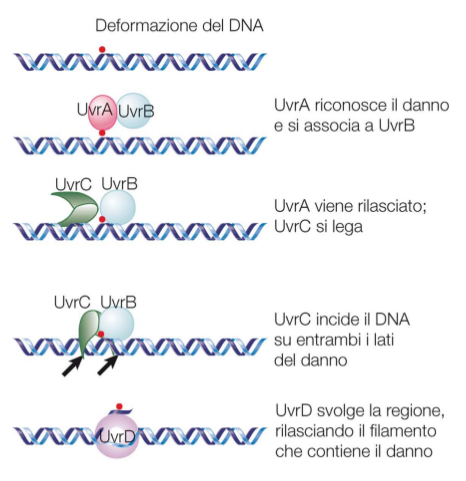
\includegraphics[scale=0.5]{img/23_NER (E coli).png}
\caption{}
\label{ner-e-coli}
\end{figure}


\subsubsection{Sistemi NER negli
eucarioti}\label{sistemi-ner-negli-eucarioti}

La riparazione per escissione di nucleotidi è coinvolta nella
riparazione di lesioni che provocano una distorsione della doppia elica
del DNA e sono causate da agenti chimico-fisici.

Il meccanismo del NER negli eucarioti si suddivide in due percorsi che
sono distinti nella prima fase per poi convergere in un meccanismo
comune:

\begin{itemize}
\itemsep1pt\parskip0pt\parsep0pt
\item
  il \textbf{GG-NER (Global Genome NER)}, che controlla l'intero genoma
  alla ricerca di eventi che causano una distorsione della doppia elica;
\item
  il \textbf{TCR-NER (Transcription-Couple Repair NER)}, che agisce su
  danno localizzati nelle regioni trascritte dalle RNA polimerasi.
\end{itemize}

Nel GG-NER il complesso proteico \textbf{XPC-hHR23B} più che ricercare
specifiche lesioni sul DNA, individua regioni in cui il corretto
appaiamento tra i due filamenti di DNA è alterato a causa di una
distorsione della doppia elica.

Nel TCR-NER diversi tipi di lesione nelle regioni trascritte determinano
un blocco delle RNA polimerasi che devono essere rimosse dal DNA per
permettere la riparazione dei danni.

Questo evento richiede due proteine specifiche del TCR-NER, chiamate
\textbf{CSA} e \textbf{CSB}.

I passaggi successivi sono comuni sia al GG-NER che al TCR-NER.

Il \textbf{complesso multiproteico TFIIH}, che contiene due polipeptidi
chiamati \textbf{XPB} e \textbf{XPD} con attività DNA elicasica, apre il
DNA per un tratto di circa 30 nt attorno alla lesione. La proteina
\textbf{XPA} conferma la presenza della lesione legandosi a essa,
altrimenti tutta la reazione termina a questo stadio. La regione del DNA
aperta dall'azione dell'elicasi è stabilizzata dal legame con la
proteina \textbf{RPA}, che è un fattore coinvolto anche nella
replicazione del DNA e che ha un'elevata affinità di legame per il DNA a
singolo filamento. \textbf{XPG} e \textbf{ERCC1/XPF} sono due
endonucleasi NER-specifiche che tagliano rispettivamente in 3' e in 5'
il filamento di DNA contenente la lesione, generando un frammento di
circa 30 nt con una estremità 3'OH nel filamento danneggiato. A questo
punto il filamento può essere riparato dai normali enzimi che replicano
il DNA copiando il filamento complementare che non è stato danneggiato.

\begin{figure}[htp]
\centering
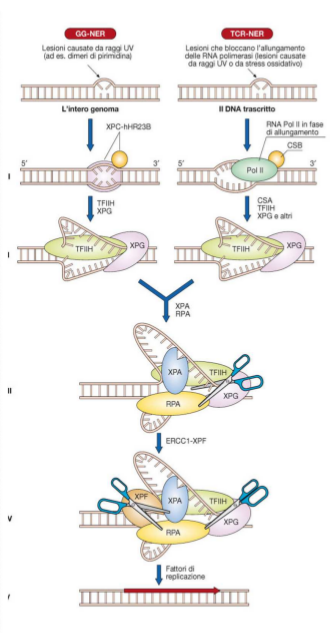
\includegraphics[scale=0.4]{img/24_NER (eucarioti).png}
\caption{}
\label{ner-eucarioti}
\end{figure}

Nell'uomo, lo \emph{Xeroderma pigmentosum}, patologia recessiva
responsabile della ipersensibilità alla luce solare, è dovuta ad un
difetto nelle riparazioni NER a causa della mutazione di uno dei geni
XPA-G coinvolti nel meccanismo.

\subsubsection{Sistemi BER negli
eucarioti}\label{sistemi-ber-negli-eucarioti}

Il primo passaggio del processo è il riconoscimento del danno da
riparare.

Nel caso di danni causati da specie reattive dell'ossigeno \textbf{DNA
glicosilasi} specifiche rompono il legame glicosidico tra lo zucchero e
la base azotata danneggiata. Questi enzimi comprimono la doppia elica
del DNA così che la base alterata viene inglobata in una cavità presente
nella struttura tridimensionale della glicosilasi. L'enzima taglia poi
il legame glicosidico che lega la base azotata alterata al deossiribosio
sul DNA. Si crea così un sito abasico (chiamato sito AP).

Successivamente una endonucleasi chiamata APE1 riconosce il sito privo
della base e incide il legame fosfodiesterico. A questo punto il
meccanismo del BER può procedere attraverso due vie:

\begin{enumerate}
\def\labelenumi{\arabic{enumi}.}
\itemsep1pt\parskip0pt\parsep0pt
\item
  \textbf{short patch BER}, preponderante nei mammiferi. Qui la DNA pol
  \(\beta\), attraverso l'attività liasica che tale polimerasi possiede,
  rimuove il deossiribosio privo della base e la stessa pol \(\beta\)
  riempie il buco di un nucleotide così creatosi. Successivamente il
  legame fosfodiesterico è saldato da una ligasi specializzata (DNA
  ligasi 3) con l'aiuto della proteina XRCC1;
\item
  \textbf{long patch BER}, prevede l'azione della DNA pol \(\delta\) e
  \(\varepsilon\) e di PCNA che allungano il 3'OH di 2-10 nt, attraverso
  una reazione di ``strand displacement''. Il filamento di DNA spelato
  via è poi tagliato da una nucleasi denominata FEN1 che riconosce la
  particolare struttura che si forma durante la reazione. La
  discontinuità sul DNA è poi saldata dall'azione della DNA ligasi 1.
\end{enumerate}

\begin{figure}[htp]
\centering
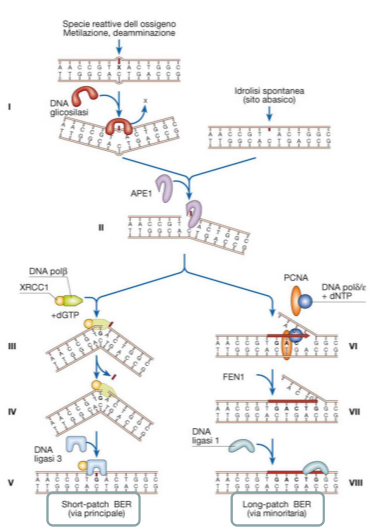
\includegraphics[scale=0.6]{img/25_BER.png}
\caption{}
\label{ber}
\end{figure}

\subsection{Riparazione di errori replicativi: MisMatch repair
(MMR)}\label{riparazione-di-errori-replicativi-mismatch-repair-mmr}

Durante la replicaizone del DNA, l'apparato replicativo può compiere
degli errori: può inserire un nucleotide che non rispetta la
complementarietà delle basi, o può provocare delezioni/inserzioni di
nucleotidi in corrispondenza di particolari sequenze sul DNA che sono
ripetute più volte.

Tali errori replicativi sono riparati da un sistema noto come MMR.

\subsubsection{MMR in E. coli}\label{mmr-in-e.-coli}

L'errore di appaiamento (mismatch) induce una distorsione della doppia
elica riconosciuta dall'omodimero \textbf{MutS} che si lega in
corrispondenza del mismatch; tale legame è stabilizzato dall'interazione
con l'omodimero \textbf{MutL}.

Un aspetto importante nel MMR è che deve essere distinto il filamento di
DNA parentale da quello di neosintesi, così che la riparazione del
mismatch avvenga su quest'ultimo.

In E. coli tale distinzione si basa sullo stato metilazione del DNA
neosintetizzato: l'adenina delle sequenze ``GATC'' del DNA di E. coli è
normalmente metilata ma, dopo la replicazione, \emph{il filamento
neosintetizzato rimane NON metilato} per una breve finestra temporale.
Il fatto che il filamento parentale sia metilato, mentre quello di
neosintesi non lo è, permette di distinguere quale filamento contenga
l'errore replicativo e debba, quindi, essere riparato.

Il complesso MutS-MutL attiva la proteina \textbf{MutH} che si lega alla
sequenza GATC metilata più vicina e, in funzione della sua attività
endonucleasica, taglia il filamento di neosintesi di fronte alla base
metilata.

L'escissione di un tratto di DNA contenente il mismatch è realizzata
tramite l'azione combinata di un'elicasi che srotola parzialmente il
filamento contenente il mismatch e la successiva azione di una
esonucleasi con la corretta polarità. Il DNA è poi riparato tramite
l'azione coordinata della DNA polimerasi III e della DNA ligasi.

\clearpage
\begin{figure}[htp]
\centering
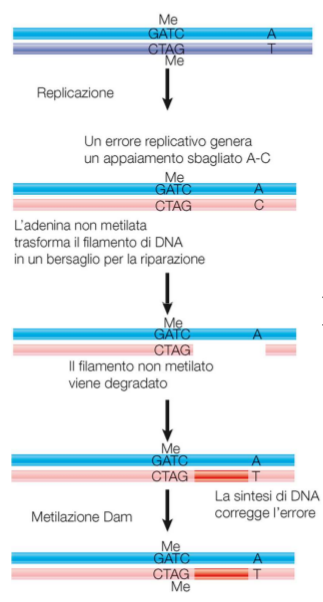
\includegraphics[scale=0.5]{img/26_MMR.png}
\caption{}
\label{mmr}
\end{figure}

\subsubsection{MMR negli eucarioti}\label{mmr-negli-eucarioti}

Negli eucarioti il meccanismo del MMR è alquanto complesso e richiede,
oltre all'azione di proteine specifiche, anche la funzione di proteine
normalmente coinvolte nei meccanismi di replicazione del DNA.

Anche negli eucarioti è necessario che venga riconosciuto il filamento
neosintetizzato. Negli eucarioti la metilazione del DNA non sembra
giocare un ruolo altrettanto importante nella discriminazione dei
filamenti, ma probabilmente sono interazioni proteina-proteina tra
fattori di replicazione e proteine dell'MMR a giocare un ruolo rilevante
nella scelta del filamento che deve essere riparato. Il meccanismo di
discriminazione sembra poi essere diverso per il filamento leading e
quello lagging.

L'apparato enzimatico che agisce durante la replicazione del DNA può
compiere alcuni errori. Per esempio, sul filamento neosintetizzato può
venire inserita una base sbagliata, oppure si possono formare delle
piccole bolle dovute allo scivolamento dell'apparato replicativo in
corrispondenza di sequenze nucleotidiche ripetute.

Tali strutture anomale sono riconosciute dai complessi MutS\(\alpha\) e
MutS\(\beta\) che reclutano, successivamente, i complessi MutL\(\alpha\)
e MutL\(\beta\) (questi complessi sono omologhi di quelli di E. coli ma
hanno maggiore specificità).

Il filamento di DNA neosintetizzato contenente gli errori replicativi
viene riconosciuto e processato da una esonucleasi (Exo1) che degrada il
filamento di DNA in direzione 5' \(\rightarrow\) 3'. Successivamente,
tramite interazioni con l'apparato di replicazione, viene
ri-sintetizzato il filamento di DNA corretto.

\begin{figure}[htp]
\centering
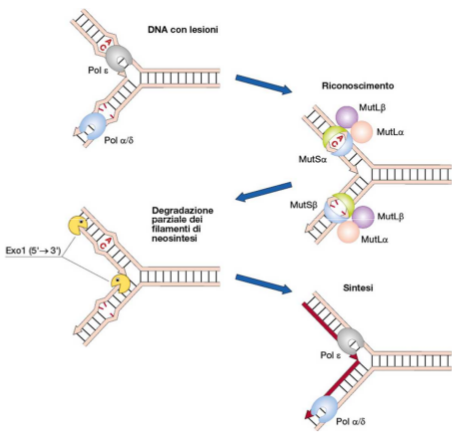
\includegraphics[scale=0.6]{img/27_MMR eucarioti.png}
\caption{}
\label{mmr-eucarioti}
\end{figure}

La perdita di questo meccanismo predispone al tumore non poliposo
ereditario del colon.

\subsection{Riparazione di rotture su entrambi i filamenti
(DSB)}\label{riparazione-di-rotture-su-entrambi-i-filamenti-dsb}

La lesione probabilemnte più pericolosa è la formazione di una rottura
su entrambi i filamenti del DNA, chiamata \textbf{DSB} o \emph{Double
Strand Break}.

La riparazione fisica dei DSB avviene principalmente mediante un
meccanismo di ricombinazione tradizionale o mediante giunzione diretta
delle estremità rotte.

Il primo meccanismo è chiamato \textbf{HR} (Homologous Recombination) e
richiede l'azione di numerose proteine ricombinative.

Nel meccanismo di HR, il complesso eterotrimerico Mre11/Rad50/Nbs1
(chiamato \textbf{MRN}) con l'ausilio di altre proteine come
\textbf{Rad51} e \textbf{Rad52}, modifica il DBS originario causando la
degradazione in direzione 5' \(\rightarrow\) 3' delle due estremità 5'
di ciascun DSB.

Si generano, così, delle regioni di DNA a singolo filamento che sono
stabilizzate dal legame della \textbf{proteina RPA}. Successivamente le
proteine Rad51, Rad52 e altre proteine ricombinative, scalzano RPA e
formano un filamento nucleoproteico in cui il DNA a singolo filamento è
ricoperto da Rad51.

L'estremità 3'OH del filamento coperto da rad51, con l'aiuto di altre
proteine ricombinative, procede ora alla ricerca di sequenze omologhe di
DNA presenti sul cromosoma omologo non danneggiato, formando la
\textbf{giunzione di Holliday}.

La perdita di Rad51 all'estremità 3'OH innesca la neosintesi di DNA. La
risoluzione degli intermedi di ricombinazione da parte di proteine
specifiche, qui indicate come risolvasi, e l'azione delle DNA ligasi
genera due molecole riparate.

\clearpage
\begin{figure}[htp]
\centering
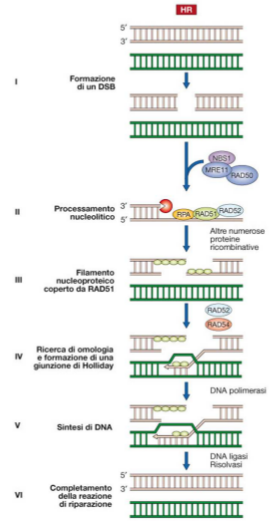
\includegraphics[scale=0.6]{img/28_DBS (HR).png}
\caption{}
\label{dbs-hr}
\end{figure}

Il secondo meccanismo è chiamato \textbf{NHEJ}. Tale reazione è
apparentemente più semplice e richiede un numero più limitato di fattori
proteici.

Nel processo NHEJ le estremità del DSB sono riconosciute da un complesso
noto come Ku70/Ku80 che interagisce con una proteina chinasi, chiamata
DNA-PK. Può accadere che le estremità del DSB siano processate in modo
limitato localmente con il possibile intervento del complesso MRN.
Infine sono reclutate proteine XRCC4 e la DNA ligasi 4 la cui azione
porta alla saldatura diretta delle estremità rotte.

\clearpage
\begin{figure}[htp]
\centering
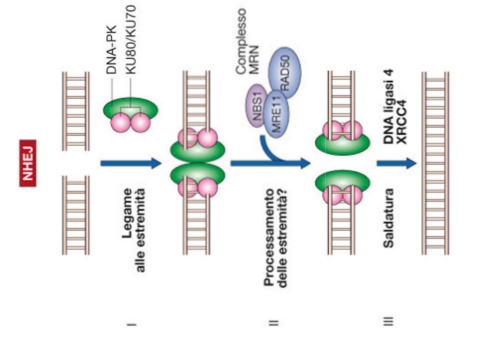
\includegraphics[scale=0.5]{img/29_DBS (NHEJ).png}
\caption{}
\label{}
\end{figure}


\subsubsection{Modello della rottura del double
strand}\label{modello-della-rottura-del-double-strand}

Un'esonucleasi genera due estremità 3'-OH sporgenti a singolo filamento.
Queste invadono una regione omologa dell'altro duplex (donatore)
(INVASIONE DEL SINGOLO FILAMENTO) dando origine a una regione di DNA
eteroduplex.

Successivamente si ha la sintesi di nuovo DNA che sostituisce il DNA
danneggiato.

La cattura della seconda estremità mediante l'appaiamento genera una
molecola in cui i due duplex sono connessi tra loro attraverso una
regione eteroduplex e due giunzioni di Holliday (incrocio).

\begin{figure}[htp]
\centering
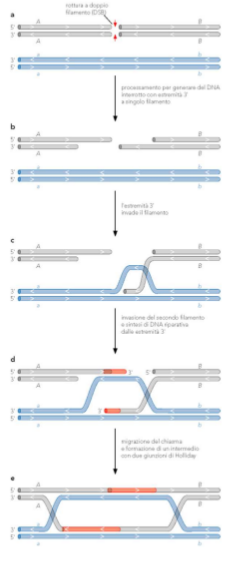
\includegraphics[scale=0.7]{img/30_Modello rottura DSB.png}
\caption{}
\label{modello-rottura-dsb}
\end{figure}

\clearpage
\subsection{Sistema di Post-Replication Repair (PRR) in E.
coli}\label{sistema-di-post-replication-repair-prr-in-e.-coli}

Il \textbf{sistema SOS} coinvolge la proteina RecA.

RecA, in E. coli, è la proteina chiave richiesta essenzialemente in
tutti i sotto-pathway ricombinativi per invadere la molecola di DNA
omologo e per promuovere l'appaiamento con il filamento complementare.

Durante la crescita in condizioni normali, l'espressione di geni SOS o
\emph{din} (Damage inducible) è repressa tramite il legame di una
proteina repressore, chiamata \textbf{LexA}, su una sequenza nota come
\textbf{``SOS box''} presente sul sito operatore di tali geni.

Come conseguenza a danni al DNA si accumulano regioni di DNA a singolo
filamento (ssDNA): RecA ha una grande affinità per l'ssDNA e il legame a
tali regioni determina la sua attivazione.

La forma attivata di RecA è in grado di legarsi al repressore LexA e di
indurre la sua distruzione tramite l'attività proteolitica che LexA
stessa possiede. Questo causa la depressione, cioè l'attivazione di una
serie di geni i cui prodotti sono richiesti per una corretta risposta a
danni al DNA.

\section{Organizzazione e impacchettamento del DNA
eucariotico}\label{organizzazione-e-impacchettamento-del-dna-eucariotico}

\subsection{La cromatina}\label{la-cromatina}

Nei nuclei delle cellule eucariotiche il amteriale genetico costituisce
la massa di cromatina la cui organizzazione è soggetta a vistosi
cambiamenti nel corso del ciclo cellulare.

Le molecole di DNA sono associate alle proteine istoniche a formare la
fibra cromatinica da 10 nm di diametro. Queste lunghe moleocle di DNA
sono organizzate in numerose anse della lunghezza media di 30-100 kpb
ancorate alla base su una struttura filamentosa chiamate \textbf{matrice
nucleare}. Queste anse costituiscono domini topologici indipendenti in
quanto capaci individualmente di mantenere o perdere superavvolgimenti.
Queste anse sono ancorate a una ``impalcatura'' centrale del cromosoma
costituita da proteine specifiche.

La fibra cromatinica risulta dall'interazione del DNA genomico con
proteine istoniche e con proteine non istoniche, e subisce notevoli
variazioni della compattazione nel corso del ciclo cellulare.

Nei nuclei interfasici i singoli cromosomi sono indistinguibili e il
materiale genetico nel nucleo si presenta come una rete diffusa di
filamenti (la cromatina) che si possono visualizzare con specifici
coloranti. La colorazione non omogenea della cromatina nei nuclei
interfasici suggerisce l'esistenza di due diverse organizzazioni
strutturali.

Nella maggior parte dello spazio nucleare le fibre cromatiniche appaiono
relativamente disperse, molto meno densamente compattate che nei
cromosomi mitotici, e prendono il nome di \textbf{eucromatina}.

In alcune regioni nucleari invece si osservano delle masse di cromatina
più compatta che prendono il nome di \textbf{eterocromatina}.
L'eterocromatina può essere distinta in due tipi:

\begin{enumerate}
\def\labelenumi{\arabic{enumi}.}
\itemsep1pt\parskip0pt\parsep0pt
\item
  \textbf{eteroctomatina costitutiva}, che resta sempre compatta e
  rappresenta regioni del genoma che, non avendo capacità codificante,
  non vengono mai espresse e che potrebbero avere un ruolo strutturale
  nel cromosoma;
\item
  \textbf{eterocromatina facoltativa}, che è tale solo in alcune
  situazioni, rappresenta regioni che hanno capacità codificante, che
  possono essere trascritta e che possono pertanto diventare
  eucromatina.
\end{enumerate}

Gli \textbf{istoni} sono proteine basiche che rappresentano i veri
costituenti strutturali della cromatina.

La cromatina presenta una struttura ripetitiva che appare come una
collana costituita da grani impilati du un filo, dove i grani
rappresentano i \textbf{nucleosomi}, le unità elementari della struttura
della cromatina.

Le unità monomeriche possono presentare lunghezze diverse dovute alla
variabilità delle dimensioni del DNA linker (DNA che lega un nucleosoma
all'altro, il ``filo'' della collana di perle). Le dimensioni del tratto
di DNA strettamente avvolto attorno al nucleosoma, infatti, sono
strettamente conservate, e sono lunghe 147 pb.

La forte interazione tra DNA e core istonico è mediata da circa 140
legami a idrogeno. Quasi tutti i legami si instaurano con gli atomi di
ossigeno dei legami fosfodiesterici vicini al solco minore; solo 7
legami vengono formati tra le proteine e le basi attraverso il solco
maggiore. Da qui la conclusione che il legame tra DNA e nucleosoma è
forte ma non è sequenza-specifico.

La natura basica degli istoni maschera le cariche negative dei fosfati,
permettendone un avvicinamento fisico, determinato dalla curvatura del
DNA, altrimenti impossibile.

Il nucleosoma è costituito da un tratto di DNA di circa 200 pb associato
con un ottamero di proteine istoniche, che consiste di due copie di
ciascuno degli istoni \textbf{H2A}, \textbf{H2B}, \textbf{H3} e
\textbf{H4}.

L'ottamero di istoni costituisce la struttura centrale o ``nucleo''
(core) del nucleosoma, a forma di cilindro appiattito del diametro di
circa 10 nm. All'intorno del cilindro la doppia elica di DNA compie
quasi due giri.

A questo nucleosoma, ma esternamente rispetto ad esso, si trova
associata una molecola dell'\textbf{istone H1}, che quindi è presente in
quantità pari alla metà di quella degli altri istoni.

L'istone H1 interagisce con il tratto di DNA tra due nucleosomi (DNA
linker) producendo una maggiore adesione del DNA all'ottamero istonico.
Il legame di H1 aumenta il compattamento del DNA sul nucleosoma,
imponendo una costrizione sugli angoli di entrata e uscita del DNA dal
nucleosoma.

Le proteine istoniche, che interagiscono con il DNA carico
negativamente, sono fortemente basiche (oltre 20\% degli aa sono Arg e
Lys). Presentano una struttura conservata costituita da tre regioni ad
\(\alpha\)-elica denominata \textbf{histone-fold} e da una coda
N-terminale.

Tutti gli istoni sono soggetti a modificazioni covalenti; la maggior
parte delle quali interessano la regione N-terminale. Modifiche
transitorie a livello di numerosi siti di acetilazione, fosforilazione e
metilazione.

In condizioni di bassa forza ioni e in assenza dell'istone H1 si osserva
la struttura meno condensata della cromatina, la ``collana di perle'',
chiamata anche \textbf{``fibra da 10 nm''}. Se analizziamo la cromatina
in condizioni più fisiologiche, essa appare come una \textbf{``fibra da
30 nm''}, chiamata anche \emph{solenoide}, in cui i nucleosomi appaiono
organizzati in una struttura elicoidale con sei nucleosomi per giro.

Il modello strutturale della cromatina che presenta il maggiore
impaccamento vede la formazione di anse bloccate alla base da una
struttura proteica, la \textbf{matrice nucleare} o l'\textbf{impalcatura
(scaffold) del cromosoma}. La \textbf{topoisomerasi II e le }proteine
SMC** \emph{(Structural Maintenance of Chromosome)} sono componenti
essenziali di quese strutture proteiche.

\section{La trascrizione}\label{la-trascrizione}

Un gene è una sequenza di DNA contenente le informazioni per la sintesi
di un prodotto indipendente (rRNA, tRNA, RNA regolatori, mRNA
\(\rightarrow\) proteina).

Si definisce \textbf{``espressione genica''} il meccanismo attraverso
cui l'informazione presente in una sequenza di DNA viene utilizzata per
produrre un RNA, o un polipeptide, mediante trascrizione e traduzione.
La relazione tra la sequenza di DNA e la sequenza aa è detta
\textbf{codice genetico}. Un gene contiene una serie di codoni che
vengono letti in maniera sequenziale a partire da un sito di inizio fino
a un sito di terminazione.

Mentre nei batteri la trascrizione è contestuale alla traduzione, dato
che non presentano una compartimentazione cellulare, negli eucarioti la
trascrizione avviene nel nucleo mentre le traduzione nel citoplasma.
L'mRNA va incontro a maturazione e solo successivamente viene tradotto.

Il processo di sintesi dell'RNA su uno stampo di DNA è chiamato
\textbf{trascrizione} e l'attore primario dell'intero meccanismo è un
enzima chiamato \textbf{RNA polimerasi}.

La RNA pol è una complessa macchina molecolare formata da varie subunità
che dopo essersi legata al DNA lo apre, creando una zona denaturata,
chiamata \textbf{bolla di trascrizione}, che fornisce all'enzima il
filamento stampo da cui è diretta la sintesi dell'RNA. La bolla si muove
con l'enzima e il DNA si apre via via che l'enzima procede e si richiude
posteriormente.

Il processo di trascrizione comprende tre diverse fasi: inizio,
allungamento e terminazione.

L'RNA prodotto non rimane appaiato al DNA, ma si stacca dallo stampo a
una distanza di pochi nucleotidi da dove è stato aggiunto l'ultimo
ribonucleotide alla catena.

Quando la doppia elica del DNA viene aperta, l'RNA pol usa uno solo dei
due filamenti come stampo.

Il filamento di DNA che funge da stampo è chiamato \textbf{filamento
stampo} ed è complementare al messaggero (RNA), mentre l'altro
filamento, che viene chiamato \textbf{fiamento non stampo} o
\textbf{codificante}, ha la stessa sequenza del messaggero, con le T al
posto delle U.

L'RNA è una catena polinucleotidica a \emph{singolo filamento}. Lo
zucchero è rappresentato dal \textbf{ribosio} anzichè 2'-deossiribosio.
Il residuo 2'-OH rende questa molecola molto reattiva (funzioni
catalitiche). Tra le basi dell'RNA troviamo l'uracile al posto della
timina. Questo filamento assorbe la luce a una lunghezza d'onda di 260
nm.

La sintesi dell'RNA è la stessa sia nei procarioti che negli eucarioti,
ma la regolazione del processo è molto più complessa negli eucarioti.

La trascrizione dei geni sia nei procarioti che negli eucarioti è
regolata da sequenze specifiche di DNA che costituiscono delle regioni
di controllo della trascrizione.

L'RNA pol sintetizza l'RNA in direzione 5' \(\rightarrow\) 3'.

L'RNA pol si lega a particolari sequenze sul DNA che si chiamano
\textbf{promotori} e che sono situate all'inizio del gene. Il promotore
contiene anche il nucleotide da cui inizia la sintesi dell'RNA, che
viene definito \textbf{sito d'inizio della trascrizione (TSS)}. La
trascrizione procede poi fino a una particolare sequenza chiamata
\textbf{terminatore} e si definisce \textbf{unità di trascrizione} il
tratto di DNA che va dal promotore fino al terminatore, espresso come
una singola molecola di RNA.

L'RNA pol, a differenza della DNA pol, non ha bisogno di un innesco per
sintetizzare un nuovo filamento di RNA. Dopo il suo posizionamento, il
gruppo 3'OH del primo nucleotide reagisce con il successivo nucleoside
5' trifosfato il cui fosfato in posizione \(\alpha\) è usato per formare
il legame fosfodiesterico, mentre i fosfati \(\beta\) e \(\gamma\) sono
rilasciati come una molecola di pirofosfato.

La bolla di trascrizione è lunga circa 25 pb, ma il tratto che forma un
ibrido tra DNA e RNA è lungo 8-9 pb.

\subsection{L'RNA polimerasi}\label{lrna-polimerasi}

La chimica della sintesi degli RNA è la stessa per tutti i tipi di RNA;
catalizza la formazione del legame fosfodiesterico utilizzando ioni
Mg\(^2\)\(^+\) quali cofattori. L'enzima è completamente processivo, per
cui un trascritto completo viene sintetizzato da un'unica RNA
polimerasi. Una volta iniziata la sintesi dell'RNA, la RNA polimerasi si
sposta unidirezionalmente lungo la catena stampo di DNA trascrivendo
l'RNA in direzione 5' \(\rightarrow\) 3'. Non necessitano di primer di
innesco e non sono dotate di attività di correzione dei trascritti.

Le RNA polimerasi sono capaci di individuare e trascrivere
selettivamente i geni interagendo, con l'ausilio di altre proteine
(elementi trans), con siti specifici del DNA (elementi cis) presenti
nella regione del promotore della trascrizione. Una volta riconosciuto
un elemento cis, la RNA polimerasi inizia la sintesi dell'RNA.

\subsubsection{L'RNA polimerasi di E.
coli}\label{lrna-polimerasi-di-e.-coli}

Il peso molecolare del nucleo (core) dell'enzima è circa di 400 kDa.

Questo oloenzima è costituito da 5 subunità:

\begin{itemize}
\itemsep1pt\parskip0pt\parsep0pt
\item
  2 subunità \textbf{\(\alpha\)}.
\end{itemize}

Queste subunità sono responsabili dell'assemblaggio del complesso e
contengono due domini che hanno funzioni diverse: il dominio C-terminale
(chiamato \(\alpha\)CTD) si lega a una zona del promotore chimata
\textbf{UP-element} (elemento a monte), mentre il dominio N-terminale è
responsabile dell'interazione con le altre subunità dell'enzima;

\begin{itemize}
\itemsep1pt\parskip0pt\parsep0pt
\item
  1 subunità \textbf{\(\beta\)}.
\end{itemize}

Questa contiene il sito catalitico, che sintetizza l'RNA, di cui fanno
parte anche due atomi di Mg\(^2\)\(^+\) essenziali per la sintesi. Uno
di questi atomi è sempre presente nel sito attivo, l'altro viene
trasportato nel complesso dai nucleotidi in entrata;

\begin{itemize}
\itemsep1pt\parskip0pt\parsep0pt
\item
  1 subunità \textbf{\(\beta\)'}.
\end{itemize}

Questa subunità si lega al DNA in maniera non specifica;

\begin{itemize}
\itemsep1pt\parskip0pt\parsep0pt
\item
  1 subunità \textbf{\(\omega\)}.
\end{itemize}

Questa subunità ha la funzione di promuovere e mantenere stabile il
complesso.

Per legarsi in maniera specifica al promotore, la polimerasi ha bisogno
di una sesta subunità, chiamata \textbf{\(\sigma\)}.

L'enzima completo
\textbf{\(\alpha\)\(_2\)\(\beta\)\(\beta\)'\(\omega\)\(\sigma\)} (o
\textbf{oloenzima}) ha un peso molecolare di circa 480 kDa.

Il fattore \(\sigma\) è costituito da 4 domini, distribuiti sul nucleo
enzimatico, in parte verso l'esterno per riconoscere e legare il
promotore e in parte nella regione interna tra le due parti della
``pinza'', formata dalle sub \(\beta\) e \(\beta\)', occupando
parzialmente il canale dove si posiziona il DNA.

Il fattore \(\sigma\) funziona come un vero e proprio fattore di
trascrizione. Con \(\sigma\) legato si riduce la capacità globale della
pol di legarsi al DNA, ma aumenta moltissimo la sua affinità per il
promotore. Questo permette all'RNA pol di essere generalmente sempre
legata al DNA (senza \(\sigma\)) e poter riconoscere con molta
precisione i promotori (quando c'è \(\sigma\)).

Al suo interno, l'RNA pol, ha un solco lungo circa 55 A con una
larghezza di circa 25 A. Esso può accogliere un tratto di DNA lungo
circa 15-16 bp di doppia elica.

Il DNA è costretto dalla struttura a fare una piegatura di quasi 90°
nella parte posteriore dell'enzima che viene definita ``muro''. Nella
parte superiore si trova il foro di uscita dell'RNA e più a destra il
canale da dove esce il DNA, che si riappaia alla fine della bolla; al
centro c'è una struttura chiamata ``timone'', che contribuisce a tenere
aperta la bolla. Nella parte inferiore c'è unas truttura a ``imbuto''
che permette l'entrata dei ribonucleosidi trifosfati.

\begin{figure}[htp]
\centering
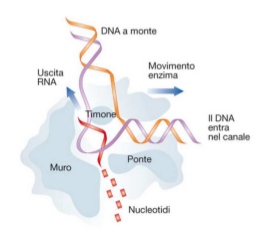
\includegraphics[scale=0.7]{img/31_RNA pol.png}
\caption{}
\label{rna-pol}
\end{figure}

\subsubsection{I promotori e il fattore sigma in
E.coli}\label{i-promotori-e-il-fattore-sigma-in-e.coli}

Per trascrivere un determinato gene l'enzima dve essere in grado di
riconoscerne il sito di inizio con grande precisione.

Questo problema è risolto da due diversi elementi: la sequenza specifica
del DNA chiamta \textbf{promotore} e la **subunità \(\sigma\) che si
associa al core della polimerasi. Il fattore \(\sigma\) riconosce il
promotore, costituito da sequenze conservate che si trovano a monte del
sito di inizio della trascrizione, ma solo quando è parte integrante
della RNA pol oloenzima.

In E. coli il fattore \(\sigma\) più usato è \(\sigma\)\(^7\)\(^0\)
(peso molecolare di 70 kDa), che riconosce un promotore costituito da
due sequenze conservate, lunghe 6 nucleotidi, che si trovano in
posizione \textbf{-10} (TATA box) e \textbf{-35}.

La sequenza consenso dell'elemento -10 è, sul filamento codificante,
TATAAT. L'elemento -35 ha come consenso la sequenza TTGACA. Il fatto che
questi elementi siano ricchi in A e T, li rende facilmente denaturabili
per formare il complesso aperto.

La forza del promotore è correlata alla maggiore o minore similitudine
delle sequenze che sono localizzate a -10 e -35. Un promotore forte
viene trascritto ogni 2 secondi, mentre uno debole viene trascritto ogni
2 minuti. La sequenza del tratto ``spacer'' (tra la regione -10 e -35)
non è importante.

Il fattore \(\sigma\) è diviso in 4 regioni, o domini, chiamati:
\textbf{\(\sigma\)\(_1\), \(\sigma\)\(_2\), \(\sigma\)\(_3\) e
\(\sigma\)\(_4\)}.

La regione \(\sigma\)\(_2\) riconosce l'elemento -10, mentre la regione
\(\sigma\)\(_4\) riconosce l'elemento -35. \(\sigma\)\(_4\) è costituita
da due \(\alpha\)-eliche che formano un dominio elica-giro-elica
(helix-turn-helix) che è tipico di molti fattori che si legano al DNA.
Un'elica interagisce con le basi esposte nel solco maggiore della doppia
elica e l'altra si posiziona sopra al solco interagendo con lo scheletro
zucchero-fosfato. L'interazione forte di \(\sigma\)\(_4\) con la regione
-35 àncora specificamente l'oloenzima al DNA, mentre la regione
\(\sigma\)\(_2\) ha il compito di promuovere l'apertura del DNA.

La regione N-terminale di \(\sigma\) ha un ruolo di regolazione molto
importante: se si elimina questo dominio, la proteina tronca è in grado
di legarsi specificamente ai promotori anche in assenza di RNA pol
``core''. Questo dato suggerisce che la regione N-terminale mascheri le
regioni \(\sigma\)\(_2\) e \(\sigma\)\(_4\) quando il fattore non è
legato all'enzima ``core'' e quando non è in grado di occupare promotori
in assenza delle subunità responsabili dell'attività di sintesi
dell'RNA. Una volta che si forma l'oloenzima, un cambiamento
conformazionale espone queste regioni rendendole in grado di legarsi al
DNA.

Il nucleo enzimatico ha una certa capacità di legare il DNA in maniera
non specifica grazie all'attrazione elettrostatica fra proteina basica e
acido nucleico. Questo legame è definito sito di legame debole. Il
fattore \(\sigma\) riduce la capacità di legare i siti deboli e
conferisce la capacità di legare i promotori. L'oloenzima riconosce un
promotore circa 10\(^-\)\(^7\) volte meglio di una sequenza non
specifica.

\subsection{Le 3 fasi della
trascrizione}\label{le-3-fasi-della-trascrizione}

\begin{enumerate}
\def\labelenumi{\arabic{enumi}.}
\itemsep1pt\parskip0pt\parsep0pt
\item
  La \textbf{fase di inizio}
\end{enumerate}

In questa fase avviene il riconoscimento del promotore e il DNA si apre
formando la bolla di trascrizione per iniziare la sintesi dell'RNA;

\begin{enumerate}
\def\labelenumi{\arabic{enumi}.}
\setcounter{enumi}{1}
\itemsep1pt\parskip0pt\parsep0pt
\item
  La \textbf{fase di allungamento}
\end{enumerate}

In questa fase la polimerasi e la bolla si muovono lungo il DNA
estendendo la catena di RNA;

\begin{enumerate}
\def\labelenumi{\arabic{enumi}.}
\setcounter{enumi}{2}
\itemsep1pt\parskip0pt\parsep0pt
\item
  La \textbf{fase di terminazione}
\end{enumerate}

In questa fase l'RNA pol si arresta al terminatore, il trascritto di RNA
si dissocia dalla polimerasi e la bolla si richiude.

Sono necessari due enzimi: la topoisomerasi, che rilascia i
superavvolgimenti negativi, e la girasi, che introduce i
superavvolgimenti negativi, per rettificare la situazione che si viene a
creare davanti e dietro la polimerasi.

Il legame che si forma inizialmente tra l'RNA pol e il promotore viene
definito \textbf{complesso chiuso} perchè il DNA non è stato ancora
aperto per formare la bolla.

Una volta che l'enzima è stabilmente legato al promotore, una serie di
cambiamenti conformazionali al suo interno promuovono l'apertura della
bolla e la formazione del \textbf{complesso aperto}. Questa apertura
rende disponibile il filamento stampo al riconoscimento complementare
dei nucleotidi.

Inizialmente l'RNA polimerasi sintetizza, senza distaccarsi dal
promotore, un frammento di RNA che viene rilasciato prima di raggiungere
i 9 nt di lunghezza. Questa \emph{sintesi abortiva} è ripetuta più volte
fino a quando, superata la lunghezza di 9 nt, si forma un ibrido DNA-RNA
(complesso ternario) sufficientemente stabile. La polimerasi può a
questo punto rilasciare il promotore e proseguire nella fase di
allungamento.

La transizione dalla fase di inizio abortivo a quella di allungamento
(non chiara) comporta un cambiamento strutturale.

Durante la fase di allungamento l'enzima si muove lungo il filamento
stampo in direzione 3' \(\rightarrow\) 5' sintetizzando la catena di RNA
dal 5' al 3' e muove con sé la bolla di trascrizione; il DNA si apre
nella direzione della sintesi e si richiude alle sue spalle, mantenendo
la bolla di una lunghezza costante.

La terminazione è l'ultima fase della trascrizione in cui l'RNA
polimerasi rilascia il filamento di RNA prodotto e si dissocia dal DNA.

\subsubsection{Passaggio complesso aperto-chiuso in E.
coli}\label{passaggio-complesso-aperto-chiuso-in-e.-coli}

Nel \textbf{complesso chiuso}: + il DNA si lega alla superficie con
\(\alpha\) e \(\sigma\); + \(\sigma\)\(_2\) e \(\sigma\)\(_4\) sono
esposti all'esterno e legano le zone -10 e -35; + l'interno del canale è
occupato da \(\sigma\)\(_1.1\).

Nel \textbf{complesso aperto} avviene l'isomerizzazione dell'RNA:

\begin{itemize}
\itemsep1pt\parskip0pt\parsep0pt
\item
  il DNA è costretto ad una piegatura di 90° che permette allo stampo di
  raggiungere il sito catalitico dove ci sono 2 Mg\(^2\)\(^+\);
\item
  avviene l'apertura dei filamenti di DNA;
\item
  \(\sigma\)\(_1.1\) si sposta;
\item
  \(\sigma\)\(_3\) e \(\sigma\)\(_4\) bloccano il canale di uscita.
\end{itemize}

Infine, nel \textbf{complesso ternario} formato da DNA, RNA ed
oloenzima;

\begin{itemize}
\itemsep1pt\parskip0pt\parsep0pt
\item
  \(\sigma\)\(_3\) e \(\sigma\)\(_4\) liberano il canale di uscita;
\item
  \(\sigma\)\(_4\) si stacca parzialmente dall'elemento -35;
\item
  l'RNA esce dal canale.
\end{itemize}

L'RNA polimerasi cambia dimensione nelle diverse fasi.

Il complesso di inizio contiene sigma e copre 75-80 bp (copre una
lunghezza da -55 a +20 sul DNA). La forma più estesa dell'enzima
potrebbe coprire solo 50 bp, per questo il DNA deve essere curvato (per
coprire una zona più estesa).

Nella fase di allungamento il complesso diminuisce le sue dimensioni
(parliamo della fase iniziale in cui l'RNA ha una lunghezza di circa di
10 bp). Può perdere \(\sigma\) e perde i contatti da -55 a -35 (servono
solo per il riconoscimento).

Infine, nella fase allungamento (RNA di 15-20b): l'enzima copre 30-40
basi.

\subsection{Terminazione della
trascrizione}\label{terminazione-della-trascrizione}

La trascrizione termina quando l'RNA pol raggiunge delle sequenze
specifiche sul DNA chiamate \textbf{terminatori}.

L'arresto impedisce l'aggiunta di nuovi nucleotidi, l'enzima si dissocia
dal DNA ed è pronto per un nuovo ciclo. È necessario che tutti i legami
che mantengono uniti i due filamenti nel tratto ibrido DNA-RNA vengano
rotti per pemettere il ri-appaiamento tra i filamenti complementari del
DNA e la dissociazione del complesso.

In E. coli esistono due meccanismi diversi per terminare la
trascrizione: in un primo caso, sequenze denominate \textbf{terminatori
intrinseci} (\textbf{Rho indipendenti}) inducono la polimerasi a
staccarsi dal complesso e a rilasciare la catena di RNA prodotto, senza
l'ausilio di alcun fattore aggiuntivo. Nel secondo caso, denominato
\textbf{terminazione Rho-dipendente}, la sequenza di terminazione non è
in grado di promuovere da sola la dissociazione del complesso, ma
necessita dell'azione della proteina Rho.

\subsubsection{I terminatori
Rho-indipendenti}\label{i-terminatori-rho-indipendenti}

Questi terminatori sono costituiti da una corta sequenza palindromica
ricca in G-C seguite da un tratto di 8-9 nucleotidi ricco in A e T.
L'RNA trascritto forma, nella regione palindromica ricca in GC, una
struttura a forcina che destabilizza, insieme al tratto di 8 U, il
complesso trascrizionale.

L'interferenza provocata dalla struttura stem-loop unita alla debolezza
del legame A:U favorisce il distacco del trascritto dallo stampo.

\subsubsection{I terminatori
Rho-dipendenti}\label{i-terminatori-rho-dipendenti}

Questo meccanismo è mediato da una proteina chiamata *``Rho* che si
trova in tutti i batteri.

Rho si associa all'RNA nascente in una regione ricca di citosine lunga
circa 40 nt, denominata \textbf{sito di utilizzo di Rho (rut)}. Questo
sito si trova a valle della regione codificante e quindi Rho non
incontrerà sul suo cammino un ribosoma che sta sintetizzando. Una volta
legato, Rho agisce come una elicasi ATP-dipendente che si muove in
direzione 5' \(\rightarrow\) 3', per traslocare verso il sito della
trascrizione e promuovere il distacco della polimerasi.

Rho ha una struttura a omoesamero e assume una forma ad anello.

Appena Rho si lega sul trascritto crescente di RNA, il singolo filamento
interagisce con il foro dell'esamero (sito di legame per l'ssDNA) e con
domini della proteina che lo circondano. Una volta formato il complesso,
il legame con l'ATP e la sua idrolisi provocano la traslocazione di Rho
lungo l'RNA, fino a che raggiunge la polimerasi e dissocia il complesso
e l'ibrido DNA-RNA. Oltre ai ``rut'', Rho utilizza per terminare la
trascrizione delle sequenze di terminazione molto simili ai terminatori
intrinseci, ma con una forcina più breve.

Rho lega l'RNA dall'estremità 3' sulla faccia esterna dei domini N-term,
mentre l'estremità 5' è legata da un sito secondario posto all'interno
dell'esamero.

Nei batteri la trascrizione è contestuale alla traduzione. L'accesso di
Rho al sito rut è mascherato dai ribosomi. Una mutazione non senso che
fa staccare i ribosomi prematuramente, fa entrare Rho che blocca la
trascrizione dei geni distali (stesso meccanismo di prima).

\begin{figure}[htp]
\centering
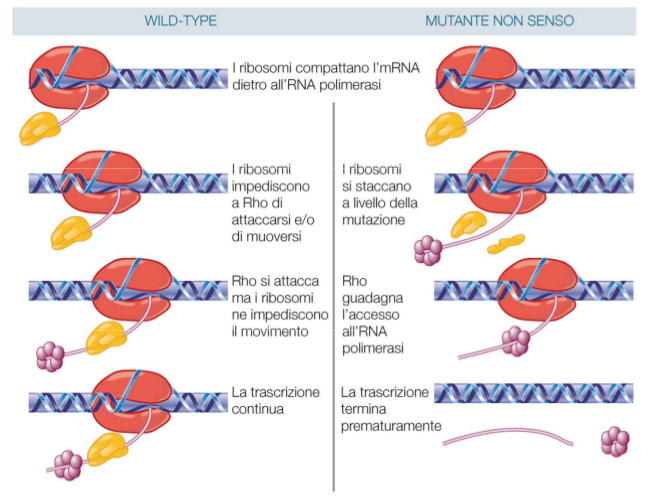
\includegraphics[scale=0.38]{img/32_Rho batterica.png}
\caption{}
\label{rho-batterica}
\end{figure}

\subsection{Differenza tra mRNA mono e
policistronico}\label{differenza-tra-mrna-mono-e-policistronico}

L'mRNA si dice \textbf{monocistronico} quando porta l'informazione per
un solo gene, ed è una caratteristica tipica degli eucarioti mentre nei
procarioti l'mRNA è molto spesso \textbf{policistronico} e cioè porta
l'informazione per più geni (il trascritto di mRNA corrispondente è in
grado di tradurre per più catene polipeptidiche diverse, in sequenza).

Un \textbf{cistrone} è una sequenza di basi nucleotidiche compresa tra
una tripletta di inizio AUG e una di stop. Il termine deriva dal fatto
che due mutazioni puntiformi diverse possono complementare (ossia dare
un fenotipo normale) solo se sono in cis, ossia nello stesso filamento
(per cui l'altro cistrone è selvatico), e non se sono in trans, in
quanto entrambi i polipeptidi risultano anormali.

La tipica organizzazione policistronica dell'mRNA dei procarioti è
dovuta alla caratteristica organizzazione dei geni in \emph{operoni},
ovvero una serie di geni disposti uno accanto all'altro lungo il
cromosoma che codificano enzimi con funzione correlata tra loro
(solitamente coinvolti nello stesso pathway) controllati da un unico
induttore e che sono trascritti su un'unica molecola di mRNA.

\subsection{La trascrizione negli
eucarioti}\label{la-trascrizione-negli-eucarioti}

Sebbene il meccanismo di trascrizione del DNA sia simile, il macchinario
necessario perchè la trascrizione avvenga è, negli eucarioti,
considerevolmente più complesso: + è necessaria una modulazione del
grado di compattezza della cromatina; + l'RNA polimerasi richiede
fattori proteici, detti \textbf{fattori di trascrizione basale}, per
legare il promotore ed iniziare la trascrizione; + esistono 3 differenti
RNA polimerasi. L'\textbf{RNA polimerasi I} trascrive i geni per l'rRNA
(localizzata principalmente nel nucleo), l'\textbf{RNA polimerasi II}
trascrive i precursori degli mRNA (localizzata nel nucleoplasma), mentre
l'\textbf{RNA polimerasi III} trascrive i geni per l'rRNA 5S, per i tRNA
e per piccoli RNA coinvolti nella formazione di mRNA maturi.

Nelle piante esistono altre due RNA pol non essenziali per la vita delle
cellule: \textbf{RNA pol IVa e pol IVb}.

Ognuna delle 3 RNA pol funziona in associazione con una serie di fattori
specifici che riconoscono elementi in \emph{cis} sul DNA nella regione
del promotore.

\subsubsection{La RNA pol I}\label{la-rna-pol-i}

La RNA pol I trascrive esclusivamente i geni per gli RNA ribosomali.

Il promotore del precursore degli rRNA è costituito da due regioni: un
tratto che si sovrappone al sito d'inizio della trascrizione TSS che
costituisce il core del promotore e un elemento più a monte, chiamato
\textbf{elemento UPE} o \textbf{UCE}.

La formazione del complesso di inizio richiede almeno due fattori
trascrizionali ausiliari, chiamati:

\begin{itemize}
\itemsep1pt\parskip0pt\parsep0pt
\item
  \textbf{UBF}, una proteina che si lega al DNA con domini multipli del
  tipo HMG e interagisce direttamente con il core del promotore e con
  l'elemento UCE;
\item
  \textbf{SL1}, un complesso multiproteico che comprende la \textbf{TATA
  Binding Protein (TBP)}, che è un componente essenziale dei complessi
  d'inizio di tutte e 3 le RNA pol eucariotiche. SL1 non si lega al DNA
  riconoscendo una sequenza specifica, ma il reclutamento sul promotore
  è mediato da interazioni specifiche con UBF. Una volta posizionato sul
  promotore, il complesso SL1 contatta direttamente il DNA e promuove la
  trascrizione, reclutando Pol I.
\end{itemize}

Un dimero di UBF si lega sia a UCE che al core del promotore,
promuovendo la formazione di un'ansa sul DNA. A questo punto interviene
SL1 che richiama Pol I sul promotore e la sintesi dell'rRNA può
iniziare.

\subsubsection{La RNA pol II}\label{la-rna-pol-ii}

Mentre nei procarioti interviene un solo fattore addizionale di
trascrizione (\(\sigma\)), negli eucarioti l'RNA pol II, per iniziare la
propria trascrizione, necessita di 2 gruppi di fattori di trascrizione
(qualsiasi proteina sia necessaria per l'inizio della trascrizione ma
non sia parte della polimerasi, è un fattore din trascrizione):

\begin{enumerate}
\def\labelenumi{\arabic{enumi}.}
\itemsep1pt\parskip0pt\parsep0pt
\item
  il primo gruppo è formato da una serie di proteine chiamate
  \textbf{fattori basali (GTF)}, richieste per reclutare l'RNA pol su
  tutti i promotori di Pol II e formare il complesso di inizio. L'RNA
  pol II associata a questi fattori costituisce l'\textbf{apparato
  basale} della trascrizione di Pol II;
\item
  il secondo gruppo è costituito da proteine chiamate \textbf{fattori di
  trascrizione regolatori} che sono responsabili della regolazione della
  trascrizione, sia come attivatori che come repressori.
\end{enumerate}

La struttura dei \textbf{promotori di Pol II} è piuttosto complessa. Il
\textbf{promotore minimo} di Pol II è costituito dal tratto di DNA
indispensabile per permettere ai fattori basali di far iniziare la
trascrizione. Tale promotore minimo contiene l'elemento chiamato
\textbf{iniziatore (INR)} da cui parte la trascrizione.

Un altro elemento molto importante è una sequenza chiamata \textbf{TATA
box} (sequenza conservata TATAAA). Tale sequenza è, in genere, preceduta
da un altro elemento chiamato \textbf{BRE} che permette il legame del
fattore basale \textbf{TFIIIB}. Un elemento chimato \textbf{DPE} è
tipicamente presente in quei promotori che non contengono le TATA box
(**TATA-less*). L'elemento \textbf{DCE} può invece essere presente in
più copie nei promotori contenenti la TATA box.

\begin{itemize}
\item
  Le TATA-box sono presenti nel 32\% dei nuclei del promotore. Esistono
  promotori TATA-less. LE TATA box sono il sito di legame per la TBP
  (TATA binding protein), una subunità di TFIID, e sono circondate da
  seq ricche in GC. Sono posizionate a -25 bp dal sito di inizio.
\item
  L'iniziatore (Inr) si trova posizionato a livello del sito di inizio,
  tendenzialmente la prima base è una A fiancheggiata da pirimidine (Py
  2 CAPy 5 ). E posizionato a -3 - +5, e viene riconosciuta da TPB e
  TAFII (???). Agisce anche in assenza della TATA box, ma se agisce in
  sinergia con quest'ultima ha una maggiore efficienza di inizio della
  trascrizione.
\item
  L'elemento DPE è formato da 7 nucleotidi. Funziona nei TATA-less e
  richiede Inr. Viene riconoisciuto da TAF9 e TAF6 (subunità di TFIID).
\item
  L'elemento DCE è legato a TAF1 e contribuisce all'attività dei
  promotori con TATA-box. È presente in tre copie.
\item
  L'elemento BRE è l'unico riconosciuto da TFIIB.
\end{itemize}

\subparagraph{I promotori della RNA pol
II}\label{i-promotori-della-rna-pol-ii}

Un promotore di Pol II è costituito da vari elementi che possiamo
suddividere in due gruppi:

\begin{enumerate}
\def\labelenumi{\arabic{enumi}.}
\itemsep1pt\parskip0pt\parsep0pt
\item
  quelli \emph{prossimali} (fino a circa 200 pb) al sito d'inizio della
  trascrizione, a cui si legano i fattori basali di trascrizione, la
  polimerasi e alcuni attivatori.
\item
  quelli \emph{distali} (circa 100 kb di distanza) ai quali si legano i
  fattori di regolazione della trascrizione.
\end{enumerate}

Nel lievito la maggior parte dei geni ha un elemento chiamato
\textbf{UAS} al quale si legano attivatori specifici per il gene posto a
valle.

I siti di riconoscimento prossimali nel promotore sono, in generale,
formati da sequenze nucleotidiche che si presentano in blocchi (box)
quali la \textbf{CAAT box} e la \textbf{GC box}. Queste sequenze fanno
parte degli elementi prossimali del promotore, funzionano in entrambi i
sensi, sono localizzate a monte del sito di inizio della trascrizione e
ne fanno aumentare la frequenza di inizio.

Alla CAAT box si lega il fattore trascrizionale noto CBF. La CAAT box
può funzionare in entrambi gli orientamenti e si ritiene che influenzi
l'efficienza di un promotore, ma non abbia un ruolo nel determinarne la
specificità trascrizionale. Alla GC box (GGGCGG) si lega il fattore Sp1,
presente in molti organismi compreso l'uomo, che è coinvolto
nell'espressione di molti geni necessari per la vitalità delle cellule
definiti \textbf{housekeeping}.

Non sempre i promotori funzionano da soli. In alcuni casi l'attività di
un promotore è aumentata enormemente dalla presenza di un enhancer. Gli
\textbf{enhancer} (amplificatori) sono elementi distali che contengono
molti elementi o sequenze di riconoscimento alle quali si legano i
fattori di trascrizione, per lo più con funzione attivatrice.

Gli enhancer possono funzionare in entrambi gli orientamenti rispetto
alla direzione della trascrizione e possono trovarsi sia a monte che a
valle del gene che controllano. Svolgono il loro ruolo attraverso
l'associazione con diverse proteine, tra cui diversi fattori coinvolti
nell'avvio della trascrizione stessa. Il complesso che viene a formarsi
(enhancer + attivatori) prende il nome di \textbf{enhanceosoma}.

Oltre agli enhancer esistono anche i \textbf{silencer} che funzionano in
modo simile, legando repressori della trascrizione (invece di
attivatori). Come gli enhancer possono trovarsi a valle o a monte dei
geni che controllano. Questi repressori possono agire in modi diversi:
possono mascherare la regione di attivazione agli attivatori, o
competere con il legame sul mediatore.

L'individuazione della funzione di sequenze di DNA coinvolte nella
regolazione della trascrizione sono state eseguite mediante diverse
tecniche, tra le quali la \textbf{mappatura per delezione}. In breve:
vengono preparate molecole di DNA con delezioni in diversi punti del
promotore del gene; le molecole modificate di DNA vengono inserite
(trasfezione) in cellule che lo inglobano nel loro DNA. Successivamente
si determina la capacità e l'efficienza della trascrizione del DNA
trasfettato nella cellule.

\subsubsection{Il complesso di pre-inizio}\label{il-complesso-di-pre-inizio}

Vediamo ora come si assembla sul promotore il complesso d'inizio della
trascrizione, promosso dai fattori basali. Questo viene chiamato
\textbf{complesso di pre-inizio} o \textbf{PIC}.

Il primo fattore a legarsi al promotore è il \textbf{TFIID} che contiene
la \textbf{TBP} insieme a numerosi \textbf{TAF} (\emph{TBP Asocciated
Factors}). I fattori TAF sono il bersaglio di proteine attivatrici che
aumentano il livello di trascrizione. I TAF associati alla TBP sono
diversi per i 3 sistemi di trascrizione Pol I, Pol II e Pol III.

TBP è una proteina molto particolare che si lega come una ``sella'' sul
DNA, interagendo con il solco minore. La molecola è un monomero con un
asse di simmetria che la divide in due regioni simmetriche e, attraverso
due loop molto conservati contenenti critici residui di fenilalanina, si
lega alla TATA box, piegando il DNA di circa 80°. Questa piegatura
facilita l'interazione di altri fattori nella regione del promotore.

Dopo TFIID si lega al complesso \textbf{TFIIA} che ha la doppia funzione
di stabilizzare il complesso TFIID-DNA e di impedire il legame di
repressori che potrebbero interferire con la formazione dle complesso di
pre-inizio.

Successivamente, al complesso si lega \textbf{TFIIB}, che ha il compito
di posizionare precisamente Pol II sul sito d'inizio ``misurandone'' la
distanza dalla TATA box.

TFIIB interagisce con la TBP e il DNA, grazie alla piegatura indotta da
TBP a monte e a valle della TATA box, è in grado d'interagire anche con
la polimerasi, che si associa al complesso aiutata da \textbf{TFIIF}.
TFIIB sembra avere un ruolo importante nelle fasi iniziali della sintesi
dell'RNA.

Il complesso TFIIB-RNA pol ha rivelato la presenza nella regione
N-terminale di TFIIB di un dominio che, attraverso un lungo loop, si
inoltra all'interno dell'enzima fino alla regione del suo sito attivo.
Questo loop, denominato \textbf{dito B} si trova nella stessa regione
dell'ibrido DNA-RNA nel complesso che sta trascrivendo e tale posizione
non interferisce, ma anzi stabilizza la struttura dell'ibrido RNA-DNA.
Quando l'RNA supera i 5 o 6 nt, deve competere con TFIIB per lo spazio
nella cavità di Pol II.

\textbf{TFIIF} si lega a Pol II quando l'enzima è ancora libero da
interazioni con altri fattori e ne impedisce il legame a regioni di DNA
diverse dal promotore. TFIIF stabilizza le interazioni della polimerasi
con TBP e TFIIB e sembra avere un ruolo nell'inizio della trascrizione.

La coda C-terminale (CTD) di Pol II, è libera e non modificata. Quando
si forma il complesso con l'RNA pol, intervengono altri due fattori:
\textbf{TFIIE} e \textbf{TFIIH}.

TFIIE ha la funzione di reclutare TFIIH nel complesso e TFIIH, che è
costituito da varie subunità, ha un duplice ruolo. Il primo è quello di
aprire il DNA mediante la sua attività elicasica ATP-dipendente e di
formare il complesso di trascrizione ``aperto''. L'altra funzione
essenziale di TFIIH è quella di \emph{fosforilare il CTD}.

Questa modificazione della coda CTD, cambiando la qualità delle
interazioni tra il CTD e i vari componenti del PIC, promuove il distacco
di Pol II dal promotore e permette l;inizio della fase di allungamento
della trascrizione.

Le modificazioni post-traduzionali della coda CTD sono anche essenziali
per reclutare, nella fase di allungamento, le varie componenti che
contribuiscono alla maturazione dell'RNA.

\begin{figure}[htp]
\centering
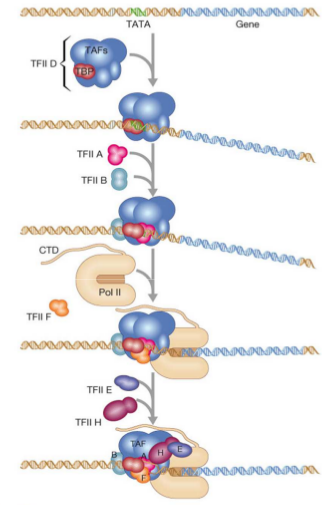
\includegraphics[scale=0.46]{img/33_Formazione PIC.png}
\caption{}
\label{formazione-pic}
\end{figure}


\subsubsection{La struttura di Pol II e la fase di allungamento
dell'RNA}\label{la-struttura-di-pol-ii-e-la-fase-di-allungamento-dellrna}

La fosforilazione del CTD, che avviene in concomitanza con l'inizio
della fase di allungamento, provoca uno scambio tra i fattori di inizio
e quelli necessari per l'allungamento e la maturazione dell'RNA. In
questo stadio molti fattori basali vengono rilasciati e fra questi anche
il mediatore (interagisce con CTD non fosforilato). La fosforilazione
del CTD serve come punto di riconoscimento e di ancoraggio per altre
proteine per agganciarsi alla pol. Il complesso di trascrizione è
costituito dalla RNApol-TFIIE-TFIIH e dai fattori di allungamento che
includono P-TEFb che fosforila CTD (in Ser2), hSPT5, TAT-SF1, TFIIS (che
impedisce le pause scorrette e correzione di bozze).

Pol II è costituita da più subunità che danno a questo enzima una forma
a ``pinza'' che si apre e si chiude sul DNA inglobandolo in una lunga
scanalatura nella struttura dell'oloenzima. La parte superiore della
``pinza'' è quella più mobile e permette l'ingresso del DNA. La brusca
curvatura che, a causa della struttura del ``muro'', il filamento è
costretto a fare, ha come risultato quello di esporre la base non
appaiata nel sito attivo, pronta ad appaiarsi con il nucleotide
successivo che entrerà nel complesso.

Come fa l'RNA pol a riconoscere il giusto nucleotide che deve essere
aggiunto alla catena di RNA?

Nell'RNA pol è presente un dominio proteico chiamato \textbf{trigger
loop} (grilletto). Questo ha il ruolo di riconoscere e discriminare il
nucleotide corretto per evitare errori nella sintesi; inoltre, promuove
la formazione del legame fosfodiesterico e l'avanzamento della
polimerasi.

Il trigger loop posiziona il nuovo NTP nel sito attivo in modo tale che,
se l'appaiamento è corretto, il nucleotide riesce a posizionarsi
correttamente rispetto al 3'OH della molecola di RNA nascente e al
nucleotide complementare nel filamento stampo del DNA. Il trigger loop
promuove l'attacco nucleofilo da parte del 3'OH e il distacco del
pirofosfato.

\subsubsection{Altri fattori proteici}\label{altri-fattori-proteici}

Il DNA è normalmente impaccato nei nucleosomi e nella cromatina.
Pertanto, l'inizio della trascrizione in vivo, richiede l'intervento di
altri fattori proteici quali il \emph{complesso mediatore},
\emph{proteine regolatrici della trascrizione} (attivatori) e
\emph{enzimi che rimodellano la cromatina}. Al contrario degli
attivatori procariotici che interagiscono direttamente con la polimerasi
posizionandola sul promotore, gli attivatori eucariotici reclutano
indirettamente la polimerasi interagendo con componenti del complesso
trascrizionale come TFIID o il complesso mediatore.

\begin{itemize}
\itemsep1pt\parskip0pt\parsep0pt
\item
  Il mediatore.
\end{itemize}

Il mediatore è un complesso proteico di grandi dimensioni che si lega al
complesso d'inizio trasportandovi l'RNA pol. Questa è legata
direttamente al mediatore che interagisce con il CTD, mascherandolo.

Il principale ruolo del mediatore è quello di fare da ponte tra gli
attivatori legati a monte e il complesso d'inizio e, inoltre, alcune sue
subunità possono avere un ruolo nella repressione della trascrizione.

\begin{itemize}
\itemsep1pt\parskip0pt\parsep0pt
\item
  Gli enhancer
\end{itemize}

L'espressione della maggior parte dei geni può essere controllata anche
dagli enhancer (intensificatori). Questi sono sequenze del DNA poste
anche a molta distanza dal promotore che possono essere spostate ed
anche ruotate di 180° senza che ciò interferisca con la capacità dei
fattori di trascrizione ad esse legate di stimolare la trascrizione.

Questi fattori proteici hanno la capacità di legare i fattori proteici
del promotore piegando ad ansa il filamento di DNA.

Ogni enhancer lega gruppi di fattori di trascrizione diversi che
rispondono a stimoli diversi e che possono agire indipendentemente.

Gli enhancer sono distanti dal gene che controllano e per evitare
interazioni errate con altri geni, si ritiene che ogni sistema
promotore/enhancer sia isolato da sequenze di confine specifiche
chiamate insulator (isolatori), alle quali si legherebbero proteine
della matrice nucleare.

Enhanceosoma = complesso di attivatori che legano l'enhancer. Questo
entra in contatto con le regioni prossimali del promotore attraverso la
formazione di un'ansa sul DNA, questi vengono a contatto col il
co-attivatore (manca il dominio di legame al DNA) che a sua volta
richiama l'RNA pol.

Il silencer è una sequenza di DNA in grado di legare dei fattori di
trascrizione detti repressori. Quando il silencer è legato dal
repressore, l'RNA polimerasi non è in grado di iniziare la trascrizione.

\subsubsection{Regolazione della trascrizione tramite
attivatori}\label{regolazione-della-trascrizione-tramite-attivatori}

\begin{figure}[htp]
\centering
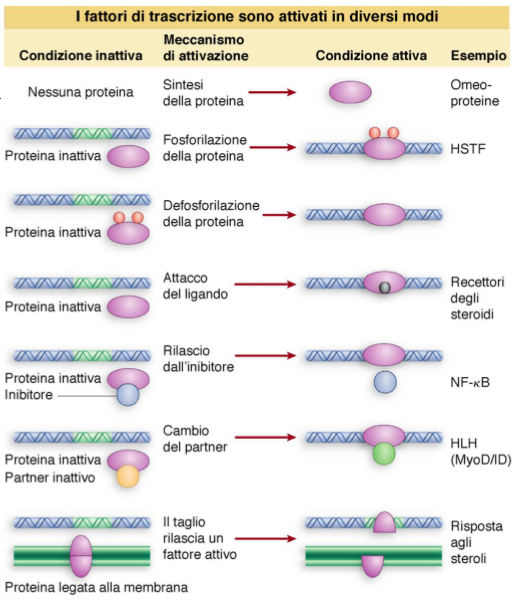
\includegraphics[scale=1.00]{img/34_attivatori.png}
\caption{}
\label{attivatori}
\end{figure}

\subsubsection{Regolazione tramite
repressori}\label{regolazione-tramite-repressori}

Il repressore può mascherare il dominio di trasporto nucleare
dell'attivatore.

\begin{figure}[htp]
\centering
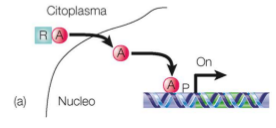
\includegraphics[scale=1.00]{img/35_Repressori (a).png}
\caption{}
\label{repressori-a}
\end{figure}

Il repressore può legare l'attivatore nascondendo il dominio di
attivazione.

\begin{figure}[htp]
\centering
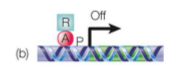
\includegraphics[scale=1.00]{img/36_Repressori (b).png}
\caption{}
\label{repressori-b}
\end{figure}

Il repressore può essere trattenuto nel citoplasma.

\begin{figure}[htp]
\centering
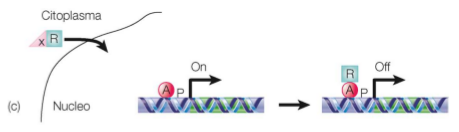
\includegraphics[scale=1.00]{img/37_Repressori (c).png}
\caption{}
\label{repressori-c}
\end{figure}

Può esserci competizione per il legame sull'enhancer.

\begin{figure}[htp]
\centering
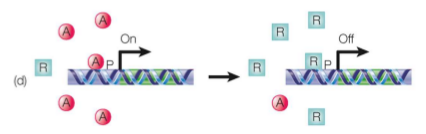
\includegraphics[scale=1.00]{img/38_Repressori (d).png}
\caption{}
\label{repressori-d}
\end{figure}

I fattori di trascrizione hanno una struttura ``modulare'', cioè sono
composti da diversi domini:

\begin{itemize}
\itemsep1pt\parskip0pt\parsep0pt
\item
  un dominio di legame al DNA (classificazione degli attivatori);
\item
  un dominio di connessione (linker);
\item
  un dominio di attivazione vero e proprio;
\item
  un dominio di dimerizzazione;
\item
  un dominio di legame ai ligandi;
\item
  un dominio di localizzazione nucleare;
\item
  un dominio di esportazione nucleare.
\end{itemize}

Ogni dominio si comporta come un modulo separato che funziona in modo
indipendente (doppio ibrido).

I fattori di trascrizione vengono suddivisi in \emph{attivatori} e
\emph{repressori} e, in base alla funzione, vengono distinti in:

\begin{enumerate}
\def\labelenumi{\arabic{enumi}.}
\itemsep1pt\parskip0pt\parsep0pt
\item
  \textbf{veri attivatori}, legano siti specifici e stabiliscono
  contatti con l'apparato basale direttamente o attraverso coattivatori;
\item
  \textbf{proteine architettoniche}, cambiano la struttura del DNA;
\item
  \textbf{antirepressori}, reclutano gli enzimi che modellano e
  modificano la cromatina.
\end{enumerate}

\subsubsection{I veri attivatori}\label{i-veri-attivatori}

La funzione dell'attivatore è quella di facilitare ed accellerare
l'assemblaggio del complesso di inizio.

Il dominio di attivazione agisce contattando:

\begin{itemize}
\itemsep1pt\parskip0pt\parsep0pt
\item
  direttamente i fattori generici di trascrizione coinvolti nelle fasi
  iniziali di assemblaggio del complesso di inizio (tipicamente TFIID,
  TFIIB o TFIIA;
\item
  il mediatore o i coattivatori.
\end{itemize}

\subsubsection{I fattori di trascrizione
architettonici}\label{i-fattori-di-trascrizione-architettonici}

Questi fattori modificano la struttura del DNA, generalmente piegandola.

Agiscono curvando il DNA; possono agire riunendo le proteine legate per
favorire la formazione di un complesso cooperativo, o curvando il DNA
nell'altra direzione per impedire la formazione del complesso.

\begin{figure}[htp]
\centering
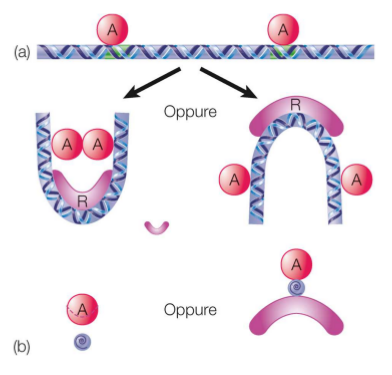
\includegraphics[scale=1.00]{img/39_Fattori architettonici.png}
\caption{}
\label{fattori-architettonici}
\end{figure}

\subsubsection{Gli antirepressori}\label{gli-antirepressori}

Nei cromosomi eucariotici il DNA è strettamente associato con gli istoni
dei nucleosomi, ed evidenze sperimentali dimostrano che queste
interazioni impediscono l'accesso al DNA dei fattori di trascrizione.

\begin{figure}[htp]
\centering
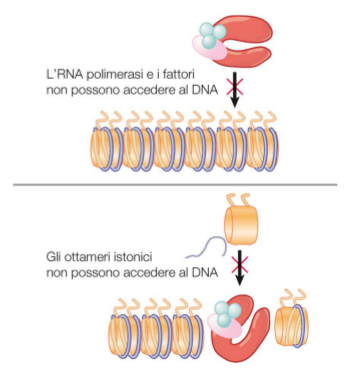
\includegraphics[scale=1.00]{img/40_Antirepressori.png}
\caption{}
\label{antirepressori}
\end{figure}

Gli antirepressori possono facilitare il legame del complesso
trascrizionale al promotore sia reclutando fattori che aggiungono gruppi
chimici alle code N-terminali degli istoni (es. l'enzima \emph{istone
acetil transferasi, HAT}, che aggiunge gruppi acetile) sia reclutando
fattori che rimodellano la cromatina (es. SWI/SNF ATP-dipendente).

\subsubsection{Modificazioni istoniche}\label{modificazioni-istoniche}

La molecola di ciascun istone del nucleosoma presenta un'estremità
N-terminale flessibile che si estende fuori dall'elica del DNA.
Modificazioni chimiche di queste code hanno un importante impatto sulla
struttura e sulla funzione della cromatina.

Le code istoniche N-terminali sono modificate covalentemente nella
porzione che esce dal core del nucleosoma. Le code sono metilate,
acetilate, fosforilate o ubiquinate su specifici residui aminoacidici.
La combinazione di specifiche modificazioni su una data coda istonica
può influenzare la funzione o l'accessibilità delle regioni di DNA
associate.

L'\emph{acetilazione} degli istoni agirebbe su due livelli molecolari
diversi:

\begin{enumerate}
\def\labelenumi{\arabic{enumi}.}
\itemsep1pt\parskip0pt\parsep0pt
\item
  impedendo la compattazione della cromatina;
\item
  favorendo lo stato di attività delle regioni eucromatiniche.
\end{enumerate}

I gruppi acetile vengono aggiunti a specifici residui di lisina (K) da
enzimi chiamati \textbf{istone acetiltrasferasi (HAT)} e tolti dalle
\textbf{istone deacetilasi (HDAT)}. Riconosciuti da bromodominio.

L'acetilazione della coda istonica permette il reclutamento di proteine
che agiscono sulla cromatina. L'acetilazione degli istoni nella
cromatina favorisce il reclutamento di proteine contenenti un
\textbf{bromodominio} che, a loro volta, possono reclutare
specificatamente altre proteine che inducono, per esempio, l'attivazione
dei geni vicini.

La \emph{metilazione} interessa i residui di Arg (fino a 2 -CH\(_3\)) e
Lys (fino a 3 -CH\(_3\)).

La metilazione della coda istonica recluta proteine che danno inizio
alla formazione di eterocromatina.

La Lys 9 metilata dell'istone H3 rappresenta un sito per il reclutamento
delle proteine che contengono un \textbf{cromodominio}. La proteina HP1
è un esempio di proteina contenente un cromodominio che aiuta l'inizio
della formazione dell'eterocromatina. Alcune proteine che contengono il
cromodominio interagiscono con altre proteine e le reclutano ai siti
della lisina 9 metilata dall'istone H3.

La metilazione è associata ad attivazione trascrizionale e
silenziamento. Es. La metilazione di Lys 9 dell'istone H3 è capace di
causare il compattamento della cromatina e il silenziamento della
trascrizione. La metilazione di Lys 4 dell'istone H3, invece, causa
attivazione della trascrizione.

\subsubsection{Modificazioni del DNA}\label{modificazioni-del-dna}

La metilazione della citosina in 5 metil-citosina, è associata a
processi di silenziamento genico.

La metilazione del DNA può reclutare proteine coinvolte nella
modificazione dell'istone e viceversa. I gruppi metile possono essere
aggiunti sia al DNA sia alle code istoniche.

I gruppi metile sul DNA reclutano le proteine leganti il metile che a
loro volta possono reclutare una deacetilasi istonica che modifica la
cromatina rimuovendo i gruppi acetile dalle code istoniche e inizia così
il silenziamento.

Le proteine che legano il metile che hanno attività metiltransferasica
possono legare i siti metilati del DNA e metilare a loro volta gli
istoni generando un segnale per il silenziamento della cromatina.

Le code istoniche metilate possono legare proteine contenenti il
cromodominio che a loro volta possono reclutare le DNA metiltransferasi
che metilano il DNA adiacente. I complessi di rimodellamento del
nucleosoma si possono legare in maniera specifica a regioni di DNA
metilato, usando le subunità che riconoscono in maniera specifica le
citosine metilate.

\subsubsection{I complessi di rimodellamento della
cromatina}\label{i-complessi-di-rimodellamento-della-cromatina}

Agiscono secondo i seguenti modelli:

\begin{enumerate}
\def\labelenumi{\arabic{enumi}.}
\itemsep1pt\parskip0pt\parsep0pt
\item
  promuovendo la mobilità dell'ottamero istonico, che scorre sul
  filamento di DNA lasciando libero il sito di attivazione della
  trascrizione TATA box (sul promotore);
\item
  inducendo un'ansa transiente nel DNA, e facendo sporgere dall'ottamero
  un sito che diventa disponibile al legame con le proteine regolatrici;
\item
  facilitando la sostituzione di un istone standard del core
  dell'ottamero con un altro che favorisce la trascrizione (H2A/H2B con
  H2AZ/H2B);
\item
  dislocando completamente l'ottamero dal DNA.
\end{enumerate}

Un esempio degli eventi che avvengono a liivello del promotore in
seguito al legame di un attivatore della trascrizione.

I fattori di trascrizione, come il recettore dei \textbf{glucocorticoidi
(GR)}, si legano al DNA e reclutano i coattivatori, che facilitano
l'assemblaggio del complesso di pre-inizio della trascrizione.

\begin{figure}[htp]
\centering
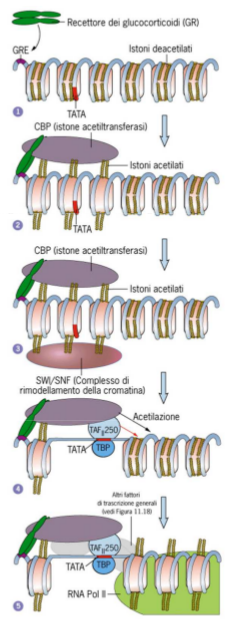
\includegraphics[scale=1.00]{img/41_Glucocorticoidi.png}
\caption{}
\label{glucocorticoidi1}
\end{figure}

Il passaggio 1 illustra la regione di un cromosoma che è in uno stato
represso a causa dell'associazione del DNA con istoni deacetilati.

Nel passaggio 2, il GR si è legato all'elemento di risposta ai
glucocorticoidi (GRE), reclutando sul DNA il coattivatore CBP. Il CBP
contiene una subuntià con attività di istone acetiltransferasi (HAT);
questi enzimi trasferiscono gruppi acetile da un donaotre (acetil CoA)
ai gruppi amminici di specifici residui di lisina. Di conseguenza, gli
istoni delle particelle core dei nucleosomi skituati nelle regioni a
monte e a valle della TATA box vengono acetilati.

Nel passaggio 3, gli istoni acetilati hanno reclutato un complesso di
rimodellamento della cromatina, chiamato SWI/SNF. Insieme, a due
coattivatori CBP e SWI/SNF hanno mdoificato la struttura della cromatina
in unos tato più aperto ed accessibile.

Nel passaggio 4, TFIID si lega a una regione accessibile del DNA. Anche
una delle subunità di TFIID (chiamata
TAF\(_I\)\$\_I\(250 o TAF1) possiede attività acetiltransferasica. Insieme, CBP e TAF\)\_I\$\$\_I\$250
destabilizzano ulteriori nucleosomi per permettetre l'avvio della
trascrizione.

Nel passaggio 5, i rimanenti nucleosomi del promotore sono stati
acetilati, la RNA polimerasi è legata ala promotore e la trascrizione
sta per iniziare.

\subsection{Domini di legame al DNA (le famiglie di fattori di
trascrizione)}\label{domini-di-legame-al-dna-le-famiglie-di-fattori-di-trascrizione}

Vediamo quali sono le strutture proteoiche più frequentemente
identificate nei domini di legame al DNA degli attivatori
trascrizionali. Questi domini sono costituiti, nella maggior parte dei
casi, da strutture ad \(\alpha\)-elica che riconoscono la sequenza
specifica di DNA interagendo con il solco maggiore della doppia elica.

Le interazioni specifiche tra DNA e proteina sono dovute principalmente
a legami idrogeno e a interazioni idrofobiche che la proteina forma con
la sequenza di DNA. È stato osservato che il riconoscimento coinvolge
in genere sequenze di 3-7 pb sul DNA. La specificità di legame è
aumentata dal fatto che per lo più gli attivatori dimerizzano e, quindi,
le sequenze di riconoscimento sono costituite da elementi doppi sul DNA.

Gli attivatori sono stati raggruppati in diverse categorie in base ai
``motivi'' con i quali si legano al DNA.

\subsection{Dita di zinco}\label{dita-di-zinco}

L'espressione ``dito di zinco'' deriva dallo schema della sua struttura,
dove un atomo di zinco coordina quattro residui di cisteine e/o
istidine, formando un'ansa che ricorda la forma di un dito.

La sequenza amminoacidica presenta, a livello di \emph{struttura
primaria}, \textbf{due cisteine} e \textbf{due istidine} distanziate tra
loro di 3, 13 e 3 residui. Nella \emph{struttura secondaria} i 4 aa (2
cys e 2 his) vanno a legare \textbf{un atomo di zinco}, formando un'ansa
di circa 12-13 aa. L'ansa è divisa in \textbf{due domini diversi}
formando, a sinistra, una struttura a \textbf{foglietto \(\beta\)} e, a
destra, un'\textbf{\(\alpha\)-elica}.

L'atomo di zinco è legato covalentemente alle due cisteine e alle due
istidine, secondo lo schema \textbf{Cys\(_2\)/His\(_2\)}.

Un intero dito di zinco è generalmente formato da 23 residui con le
cisteine e le istidine molto conservate alla sua base.

La punta dell'ansa è formata in genere da amminoacidi idrofobici che
stabilizzano la struttura dell'ansa, mentre l'\(\alpha\)-elica va a
interagire con il solco maggiore della doppia elica del DNA; linker di
7-8 aa separano più dita adiacenti.

Gli attivatori di questa classe hanno da un minimo di 2 ``dita'' fino a
un massimo di 37 ``dita'' (TFIIIA ne presenta 9, mentre Sp1 ne presenta
3).

\begin{itemize}
\item
  L'attivatore di lievito Gal4, che attiva il gene GAL1, si lega al DNA
  come un dimero tramite due dita di zinco che riconoscono elementi di
  17 pb.
\item
  Anche i recettori degli ormoni steroidei presentano una struttura a
  dita di zinco. Questi recettori dimerizzano e riconoscono il loro sito
  di legame sul DNA costituito da 2 sequenze di 6 nt orientate in
  direzione opposta, con una spaziatura di 3 nt tra loro. In queste
  proteine, che hanno dita di zinco del tipo Cys\(_2\)/Ciys\(_2\), non
  si riscontrano ripetizioni in serie della struttura a dito.
\end{itemize}

Questi recettori presentano una regione N-terminale, una regione
conservarta che lega il DNA, e una regione C-terminale che lega
l'ormone.

Le diverse attività biologiche dei vari steroidi dipendono da quali geni
vengono ``accesi'' dagli attivatori con cui ogni steroide interagisce.

Come avviene l'attivazione di un gene da parte di un ormone steroideo?
Ad esempio, nel caso del glucocorticoide cortisolo, l;ormone entra nella
cellula dal fluido extracelloulare, diffonde attraverso il doppio strato
lipidico ed entra nel citoplasma, qui si lega ad un recettore specifico.
Il legame dell'ormone cambia la conformazione del recettore e ne
determina la traslocazione nel nucleo, dove agisce da fattore di
trascrizione legandosi ad un elemento di risposta ai glucocorticoidi
(GRE) del DNA. Il recettore dei glucocorticoidi si lega al GRE come
dimero, attivando la trascrizione del DNA, e portando alla sintesi di
specifiche proteine nel citoplasma.

\begin{figure}[htp]
\centering
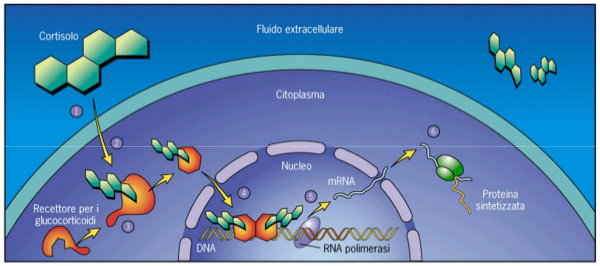
\includegraphics[scale=1.00]{img/42_Glucocorticoidi.png}
\caption{}
\label{glucocorticoidi2}
\end{figure}

Il legame dei recettori degli steroidi alla sequenza bersaglio è indotto
dall'interazione con il ligando. Gli steroidi attraversano la membrana
per semplice diffusione (sono idrofobici). Legano il recettore nella
regione C-terminale della proteina con meccanismi che dipendono dai
singoli recettori: il recettore diventa capace di legare la sua sequenza
bersaglio sul DNA, che di solito si trova in un enhancer. Come dimero
(omo o etero) il recettore/attivatore lega una singola sequenza di
riconoscimento. Il dominio di legame al DNA ha 2 ``dita di zinco'' di
tipo leggermente diverso, con un consenso
Cys-X\(_2\)-Cys-X\(_1\)\(_3\)-Cys-X\(_2\)-Cys, chiamato ``dito di zinco
Cys\(_2\)/Cys\(_2\)''. I siti di legame al DNA sono corti e palindromi,
AGAAAnnnTGTTCT. Ciascun monomero lega un mezzo sito. A questo punto, il
promotore associato all'enhancer è attivato e la trascrizione inizia.

\subsection{Elica-ansa-elica (helix-loop-helix,
HLH)}\label{elica-ansa-elica-helix-loop-helix-hlh}

Il dominio HLH, ha una struttura monomerica caratterizzata da \textbf{2
\(\alpha\)-eliche anfipatiche} (presentano residui idrofobici su una
faccia e residui carichi sull'altra) connesse da un'ansa.

In generale un monomero è costituito da circa 40 aa e l'elica più lunga
contiene, nella regione N-terminale, un dominio basico che permette di
interagire con il DNA. La formazione di un dimero, che rappresenta la
struttura in grado di legare il DNA, avviene mediante interazioni tra le
facce idrofobiche dei due monomeri. Questi attivatori sono anche
chiamati \textbf{BHLH} \emph{(Basic Helix-Loop-Helix)}

Le proteine HLH che non hanno la regione basica delle BHLH impediscono
al partner nell'eterodimero di legarsi al DNA.

\begin{figure}[htp]
\centering
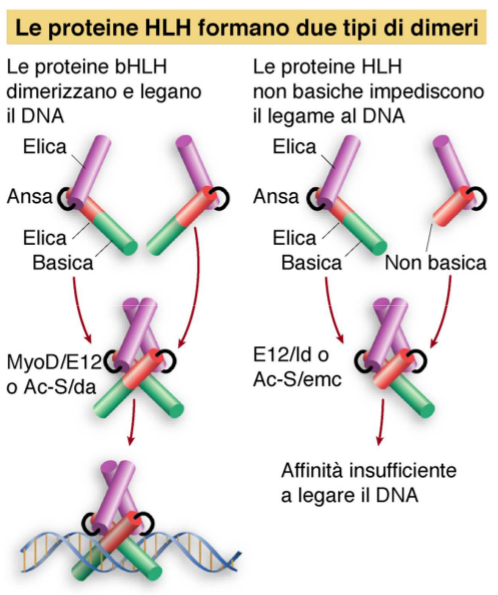
\includegraphics[scale=1.00]{img/43_HLH.png}
\caption{}
\label{hlh}
\end{figure}

\subsection{Elica-giro-elica (helix-turn-helix,
HTH)}\label{elica-giro-elica-helix-turn-helix-hth}

La struttura generica del motivo HTH è costituita da 3 \(\alpha\)-eliche
ripiegate in cui l'elica 3, chiamata anche \textbf{elica R (elica di
riconoscimento)}, si posiziona nel solco maggiore del DNA. I residui
amminoacidici dell'elica R che si affacciano sul DNA interagiscono
specificamente con le basi della sequenza di riconoscimento. La
sostituzione di una si queste basi abbassa notevolmente l'affinità della
proteina per quella sequenza.

In alcuni casi le \(\alpha\)-eliche possono essere 2 o 4, sempre con
un'elica R che interagisce nel solco maggiore della doppia elica.

Di questa famiglia di attivatori fa parte anche l'\textbf{omeodominio
(HD)}.

L'omeodominio è una sequenza conservata di 60 amminoacidi che viene
chiamata \textbf{HOMEBOX}, presente in alcuni attivatori e che prende
contatto con il solco maggiore del DNA. Attivatori contenenti un
omeodominio sono presenti in tutti gli eucarioti. Le proteine possono
essere sia attivatori che repressori.

L'omeodominio è costituito da 3 \(\alpha\)-eliche strutturate come nel
dominio HTH, in cui l'elica R contatta il solco maggiore del DNA
riconoscendo una sequenza di 6pb. L'omeodominio contiene anche un
braccio flessibile, non strutturato, che interagisce specificamente con
il solco minore del DNA.

\subsection{Domini a cerniera di leucina (leucine
zipper)}\label{domini-a-cerniera-di-leucina-leucine-zipper}

Questi attivatori sono dimeri formati da due lunghe strutture ad
\(\alpha\)-elica, ciascuna delle quali contiene, contemporaneamente, un
dominio di dimerizzazione e un dominio basico di legame al DNA.
Quest'ultimo è formato dalla parte terminale delle due \(\alpha\)-eliche
che si inseriscono nel solco maggiore della doppia elica ma sulle facce
opposte del DNA, dove gli elementi di risposta sono costituiti da una
coppia di sequenze di 4 pb con orientamento opposto, distanziati da un
nucleotide.

Il dominio di dimerizzazione presenta, a livello della struttura
primaria, un residuo di leucina ogni 7 aa. In questo modo, una volta
acquisita la struttura ad \(\alpha\)-elica, e poichè un giro di elica
corrisponde a circa 3,5 residui amminoacidici, le leucine vengono a
trovarsi, ogni due giri, sullo stesso lato dell'elica. L'assemblaggio
della struttura dimerica è dovuto ai legami idrofobici tra le leucine
che protrudono dalle due \(\alpha\)-eliche.

Si forma una \textbf{struttura a Y}, in cui il gambo della Y è formato
dalla serratura di leucine, e le due regioni basiche si biforcano
simmetricamente formando le braccia che legano il DNA. La sequenza
bersaglio di queste proteine è palindroma.

\subsection{Gli elementi di risposta}\label{gli-elementi-di-risposta}

Gli elementi di risposta sono formati dalla sequenza di un promotore
eucariotico che viene riconosciuta da un fattore trascrizionale
specifico. Rappresentano il sito di riconoscimento di specifici fattori
di trascrizione.

Questi elementi identificano gruppi di promotori o di enhancer soggetti
a controllo coordinato. Questo avviene grazie al fatto che contengono
brevi sequenze consenso, le cui copie presenti in geni diversi sono
strettamente correlate, ma non necessariamente identiche.

La presenza di un singolo elemento di solito è sufficiente per attivare
la risposta, ma talvolta ne esiste più di una copia.

Questi elementi non si trovano a distanze fisse dal sito di inizio e
possono trovarsi sia sul promotore che sull'enhancer, o in entrambi. La
regione legata dal fattore si estende per una breve distanza su entrambi
i lati della sequenza consenso.

La differenza rispetto agli attivatori costitutivamente attivi è che la
proteina è attiva o disponibile solo quando il gene è acceso.

Esempi di questi elementi sono:

\begin{itemize}
\itemsep1pt\parskip0pt\parsep0pt
\item
  \textbf{HSE}, si lega al fattore di risposta per gli shock termici;
\item
  \textbf{GRE}, è l'elemento di risposta ai glucocorticoidi;
\item
  \textbf{SRE}, è l' elemento di risposta al siero;
\item
  \textbf{HSE}, è una sequenza consenso riconosciuta dall'attivatore
  HSTF.
\end{itemize}

L'attivatore HSTF attivo, ovvero fosforilato, attiva circa 20 geni. Nei
procarioti il fattore corrispondente è \(\sigma\) 32.

I fattori specifici di trascrizione legano i **``response elements (RE,
elementi responsivi)**.

I response elements sono brevi sequenze di DNA all'interno di una
regione promotore di un gene, capaci di legare specifici fattori di
trascrizione e regolare la triscrizione dei geni.

In condizioni di stress, una proteina attivatrice della trascrizione
lega l'elemento responsivo e stimola la trascrizione. Se la stessa
seuqenza dell'elemento responsivo si trova nella zona di controllo di
più geni, allora questi geni saranno attivati dallo stesso stimolo
producendo in questo modo una risposta coordinata.

\subsection{Controllo combinatoriale della
trascrizione}\label{controllo-combinatoriale-della-trascrizione}

Se la stessa sequenza di riconoscimento si trova su geni diversi, è
possibile ottenere il controllo di più geni tramite l'utilizzo di un
numero limitato di fattori.

Inoltre l'eterodimerizzazione aumenta la quantità di fattori di
trascrizione diversi che possono essere generati da un numeri limitato
di polipeptidi.

\subsubsection{Gli elementi di controllo della trascrizione nei geni
trascritti dalle RNA pol
I}\label{gli-elementi-di-controllo-della-trascrizione-nei-geni-trascritti-dalle-rna-pol-i}

Le RNA polimerasi I trascrivono gli rRNA 28S, 18S e 5,8S.

Il loro promotore contiene due regioni (è bipartito):

\begin{enumerate}
\def\labelenumi{\arabic{enumi}.}
\itemsep1pt\parskip0pt\parsep0pt
\item
  il \textbf{``core''}, che si estende da -45 a +20 e ricco in GC (solo
  vicino al sito di inizio una regione ricca in AT);
\item
  la regione a monte, chiamata \textbf{UPE} o \textbf{UCE} che si
  estende da -180 a -107 e ricca in GC.
\end{enumerate}

Le RNA pol I presentano due fattori trascrizione:

\begin{enumerate}
\def\labelenumi{\arabic{enumi}.}
\itemsep1pt\parskip0pt\parsep0pt
\item
  \textbf{SL1} che lega il core del promotore. Questo è un fattore di
  posizionamento formato da 4 subunità (TBP, ovvero una TATA binding
  protein che non lega direttamente il DNA, e altri TF);
\item
  \textbf{UBF} che lega la regione UPE. Questo fattore presenta due
  funzioni: stimola il rilascio dal promotore della polimerasi, e
  stimola SL1.
\end{enumerate}

UBF lega UPE promuovendo la formazione di un'ansa. Contemporaneamente
richiama SL1 che prende contatto con il DNA. Successivamente viene
reclutata la RNA polimerasi I che inizia la trascrizione.

\begin{figure}[htp]
\centering
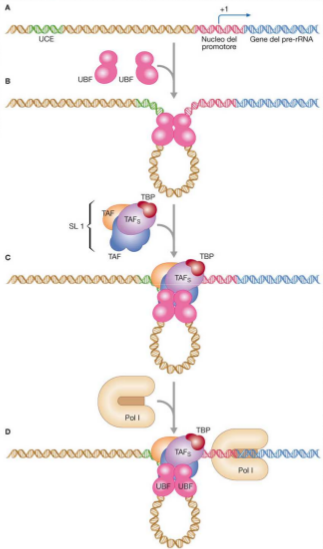
\includegraphics[scale=1.00]{img/44_Elementi controllo RNA pol I.png}
\caption{}
\label{elementi-controllo-rna-pol-i}
\end{figure}

\subsection{Elementi di controllo della trascrizione nei geni
trascritti dalle RNA pol
III}\label{elementi-di-controllo-della-trascrizione-nei-geni-trascritti-dalle-rna-pol-iii}

Le RNA pol II presentano 2 classi generali di promotori:

\begin{enumerate}
\def\labelenumi{\arabic{enumi}.}
\itemsep1pt\parskip0pt\parsep0pt
\item
  i promotori per rRNA 5S e tRNA, i quali sono \textbf{interni} (cioè si
  sovrappongo alle regioni trascritte) e contengono degli elementi
  (\textbf{box}) di controllo (si trovano a valle del sito di inizio
  della trascrizione). Questi promotori hanno una struttura bipartita
  con corte sequenze consenso separate da una regione variabile e
  localizzate all'interno dell'unità di trascrizione. Possono essere di
  \textbf{tipo1} (box A e box C) e di \textbf{tipo 2} (box A e box B);
\item
  i promotori per snRNA invece, contengono elementi di controllo tra cui
  un tipico elemento TATA a monto del sito di inizio della trascrizione.
  Oltre a questa sequenza, che permette il legame specifico di TBP,
  questi promotori pososno contenere anche le sequenze consenso per il
  legame degli elementi PSE e Oct. Questi ultimi sono riconosciuti anche
  nei promotori per snRNA trascritti dalla RNA pol II. Questi promotori
  sono detti di \textbf{tipo 3}.
\end{enumerate}

\begin{figure}[htp]
\centering
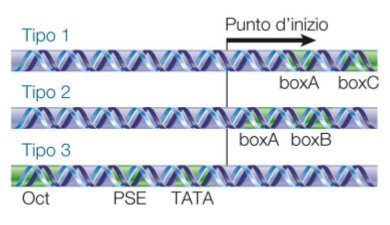
\includegraphics[scale=1.00]{img/45_Elementi controllo RNA pol II.png}
\caption{}
\label{elementi-controllo-rna-pol-ii}
\end{figure}

\subsubsection{I promotori di TIPO 1}\label{i-promotori-di-tipo-1}

\textbf{TFIIIA} permette il posizionamento di \textbf{TFIIIC} sul
\emph{box C}, che a sua volta richiama \textbf{TFIIIB} sul sito di inzio
della trascrizione.

TFIIIA e TFIIIC sono dei fattori di assemblaggio il cui compito è di
posizionare in modo corretto TFIIIB sul TSS.

La funzione della componente TBP, che fa parte di TFIIIB, è di reclutare
Pol III precisamente sul sito di inizio.

\subsubsection{I promotori di TIPO 2}\label{i-promotori-di-tipo-2}

Il fattore \textbf{TFIIIC} si lega agli elementi interni denominati
\textbf{boxA} e \textbf{box B}. Questo legame, che è indipendente da
altri fattori, richiama sul promotore \textbf{TFIIIB}. Questo è composto
da diverse subunità tra le quali TBP. La formazione di questo complesso
richiama la RNA pol III su TSS (Transcription Start Site).

Una volta legato TFIIIB, TFIIIA e TFIIIC possono allontanarsi. Il solo
TF di inizio per la RNA pol III è quindi TFIIIB!

\section{Modificazioni chimiche
dell'RNA}\label{modificazioni-chimiche-dellrna}

Esistono motleplici livelli di regolazione dell'espressione genica negli
eucarioti:

\begin{itemize}
\itemsep1pt\parskip0pt\parsep0pt
\item
  \textbf{meccanismi epigenetici}, consistono in un controllo a lungo
  raggio mediante rimodellamento della struttura della cromatina;
\item
  \textbf{controllo trascrizionale}, consiste nel legame di fattori
  trascrizionali tessuto specifici, nel legame diretto di ormoni, di
  fattori di crescita o di elementi intermedi a elementi responsivi di
  geni inducibili;
\item
  \textbf{controllo post-trascrizionale}, consiste nello splicing
  alternativo, nella poliadenilazione alternativa e dell'RNA editing
  tessut-specifico;
\item
  \textbf{controllo del trasporto};
\item
  \textbf{controllo della stabilità del trascritto};
\item
  \textbf{controllo traduzionale};
\item
  \textbf{controllo post-traduzionale}.
\end{itemize}

La forma più semplice di un gene è data da un segmento di DNA colineare
con una proteina. I geni batterici sono generalmente di questo tipo, ma
anche la maggior parte dei geni degli eucarioti unicellulari ed
oligocellulari.

A livello di DNA, la sequenza di un gene piò contenere dei tratti di
sequenza interposti ce non compaiono poi nel trascritto maturo
funzinale. Tali sequenze interposte sono state chiamate
\textbf{introni}, mentre i tratti di sequenza che, unendosi, vanno a
formare il trascritto maturo sono stati chiamati \textbf{esoni}. Geni di
questo tipo sono stati chiamati \textbf{geni discontinui} o
\textbf{interrotti}.

In questo caso il prodotto della RNA polimerasi è detto
\textbf{trascritto primario (pre-RNA)} e ha la stessa organizzazione del
gene Il \emph{pre-RNA} è molto instabile ed ha una maggiore complessità
di sequenza rispetto all'mRNA maturo. L'insieme di questi trascritti è
definito \textbf{hnRNA (RNA eterogeneo nucleare)}.

\emph{Introni} = sequenze che vengono rimosse, durante la maturazione,
dal trascritto primario.

\emph{Esoni} = sequenze che si ritrovano nell'RNA maturo.

Nei geni unmani il numero di introni può variare da nessuno fino a oltre
300 (gene per la titina)

La lunghezza complessiva degli esoni è pari a circa il 10\% della
lunghezza complessiva degli introni.

La maturazione del trascritto primario a mRNA avviene nel nucleo e
richiede 3 eventi:

\begin{itemize}
\itemsep1pt\parskip0pt\parsep0pt
\item
  un \textbf{capping al 5'};
\item
  una \textbf{poliadenilazione al 3'};
\item
  un fenomeno di \textbf{splicing}.
\end{itemize}

Allungamento, terminazione e maturazione sono fenome interconnessi. La
RNA polimerasi, mentre trascrive, porta sulla sua coda anche proteine di
modificazione del pre-mRNA che vengono trasferite sull'RNA nascente al
momento opportuno.

\subsection{\texorpdfstring{L'aggiunta del
``cap''}{L'aggiunta del cap}}\label{laggiunta-del-cap}

Gli mRNA eucariotici vengono generati nel processo trascrizionale
all'intenro del nucleo a partire da un RNA precursore (hnRNA) che deve
poi subire un processo di maturazione.

Il \textbf{capping} consiste nell'aggiunta di uno specifico nucleotide
modificato con le funzioni di protezione e riconoscimento all'estremità
5' dell'mRNA precursore.

Il cap è costituito da \textbf{7-metilguanosina (m\(^7\)G)} legata al
nucleotide iniziale del trascritto mediante un insolito legame 5'-5'. La
sequenza degli eventi che porta all'aggiunta del cap richiede 4 diverse
attività enzimatiche:

\begin{enumerate}
\def\labelenumi{\arabic{enumi}.}
\itemsep1pt\parskip0pt\parsep0pt
\item
  una RNA trifosfatasi rimuove il \(\gamma\)-fosfato all'estremità 5'
  del trascritto nascente;
\item
  una guanilil transferasi aggiunge un GMP, derivato dal GTP, al
  difosfato rimasto all'estremità del trascritto formando un legame
  trifosfato 5'-5';
\item
  una RNA metil transferasi del trascritto trasferisce un gruppo
  metilico dall S-adenosilmetionina (AdoMet) all'azoto in posizione 7
  (N\(_7\)) della guanosina aggiunta nella reazione precedente;
\item
  un'altra metil transferasi usa un'altra molecola di AdoMet per
  metilare il 2'-OH del primo nucleotide del trascritto.
\end{enumerate}

Nel \textbf{cap1}, presente sia in RNA cellulari che virali, risulta
metilato il 2'-OH del primo nucleotide del trascritto , tipicamente
un'adenina, che a sua votla può essere metilata in posizione 6.

Nel \textbf{cap2}, presenta solo negli RNA cellulari, risulta metilato
al 2'-OH anche il secondo nucleotide del trascritto.

Nel \textbf{cap0}, presente solo negli RNA virali, non vi sono
nucleotidi metilati oltre alla 7-metilguanosina.

Per alcuni RNA, come snRNA o snoRNA, si osserva una ipermetilazione del
m\(^7\)G cap, localizzata nel citoplasma, per formare
\textbf{2,7,7-trimetilguanosina}.

Il cap viene aggiunto nelle prime fasi della trascrizione, dopo che il
trascritto nascente ha raggiunto la lunghezza di 20-40 basi, ma prima
dell'occorrenza degli altri processi di maturazione.

Il posizionamento del complesso dei fattori proteici necessari per la
formazione del cap al 5' del trascritto è assistito dal dominio
C-terminale della RNA pol II (CTD). Il CTD è coinvolto nei vari passaggi
di maturazione del trascritto di Pol II.

Nella transizione tra la fase di inizio e quella di allungmaento della
trascrizione, il CTD della RNA pol II viene fosforilato da TFIIH sulla
serina 5 dell'eptapeptide ripetuto YSPTSPS. La coda viene poi
fosforilata in Ser2 da una chinasi (pTETb) associata alla RNA pol II
attivando l'allungamento, lo splicing e la poliadenilazione.

Il CTD fosforilato (P-CTD) recluta il complesso proteico coinvolto nel
capping.

Il cap svolge diverse funzioni:

\begin{itemize}
\itemsep1pt\parskip0pt\parsep0pt
\item
  protegge l'mRNA dalla degradazione;
\item
  aumenta l'efficienza della traduzione;
\item
  facilita il trasporto dell'mRNA dal nucleo al citoplasma;
\item
  contribuisce ad aumentare l'efficienza del processo di splicing.
\end{itemize}

La defosforilazione della posizione 2 richiama gli enzimi per la
poliadenilazione, mentre la defosforilazione della Ser5 ne provoca la
dissociazione.

\subsection{La poliadenilazione e terminazione della trascrizione
degli mRNA
eucariotici}\label{la-poliadenilazione-e-terminazione-della-trascrizione-degli-mrna-eucariotici}

Quando l'RNA pol II raggiunge la fine di un gene e trascrive uno
specifico motivo di sequenza, denominato \textbf{segnale di
poliadenilazione}, si innescano i meccanismi che portano alla
terminazione del processo trascrizionale, al taglio del pre-mRNA e
all'aggiunta dei una coda di poli(A) all'estremità 3'.

La trascrizone del segnale di poliadenilazione attiva il reclutamento da
parte della coda CTD dell'RNA pol II di complessi proteici denominati
\textbf{CPSF (Cleavage and Poly(A)denylation Specifity Factor)} e
\textbf{CstF (Cleavage stimulation Factor)}. Il segnale di
poliadenilazione, che più viene chiamato \textbf{segnale di cleavage} o
\textbf{taglio}, è costituito normalmente dalla sequenza esanucleotidica
\textbf{AAUAAA}, localizzata a 5-30 nt a monte del sito di taglio e
poliadenilazione e viene riconosciuto dal complesso CPSF.

L'apparato di poliadenilazione non riconosce l'estremità 3' terminale
del trascritto ma il segnale di poliadenilazione, mentre l'RNA
polimerasi II è ancora nella fase di allungamento del trascritto.

Il segnale di poliadenilazione è necessario, ma non sufficiente,
affinchè il processo di poliadenilazione possa aver luogo in modo
efficiente. Infatti, 20-30 nucleotidi a valle del sito di
poliadenilazione si osserva una sequenza ricca in G + U (o solo U) che
aumenta sensibilmente l'efficienza della poliadenilazione. QUesta zona è
riconosciuta da CstF.

I complessi CPSF e CstF agiscono in modo cooperativo insieme ad altri
due fattori proteici, necessari pe ril taglio dell'mRNA, denominati
\textbf{cleavage factor I e II (CFI e CFII)}, oltre ala poli(A)
polimerasi che catalizza l'aggiunta della cosa di poli(A).

La poliadenialzione avviene in due fasi:

\begin{itemize}
\itemsep1pt\parskip0pt\parsep0pt
\item
  una fase di inizio, nella quale si ha l'aggiunta della prima decina di
  adenine (dipendente dal segnale di poliadenilazione). Richiede PAP e
  CPSF;
\item
  una fase di allungamento nella quale vengono rapidamente aggiunte
  ulteriori 200-250 adnine (indipendente dal segnale di
  poliadenilazione). Richiede PAP, \textbf{PABN1 (Poly(A) Binding
  Protein Nuclear 1}, lega il tratto poli(A) mediante un meccanismo
  sconosciuto e limita l'attività di PAP a circa 200 A)
\end{itemize}

La fase di inizio richiede anche l'azione della \textbf{poli(A)
polimerasi (PAP)} oltre che di CPSF. Il PAP utilizza ATP come substrato,
non richiede una sequenza stampo (no sequenza su DNA), e ha la stessa
chimica della RNA polimerasi II.

La poliadenilazione è necessaria per la maturazione dell'mRNA. La
\textbf{cardicepina} impedisce la comparsa dell'mRNA citoplasmatico, ma
la trascrizione non viene inibita.

L'mRNA maturo viene rilasciato dalla polimerasi, che per un tratto
continua la sintesi di RNA sullo stampo, e viene poi trasferito dal
nucleo al citoplasma (dove sarà tradotto). Il polyA nel citoplasma viene
accorciato da RNAasi (accorciamento-sintesi nel citoplasma).

Sono stati proposti due modelli di terminazione:

\begin{enumerate}
\def\labelenumi{\arabic{enumi}.}
\itemsep1pt\parskip0pt\parsep0pt
\item
  \textbf{modello siluro}. Un'esonucleasi specifica si legherebbe al 5'
  dell'RNA che continuerebbe ad essere trascritto dopo il taglio. La
  degradazione sarebbe però più veloce della sintesi e l'esonucleasi
  raggiungerebbe dunque l'RNA pol ed inducendo il rilascio del
  trascritto;
\item
  \textbf{modello allosterico}. Il taglio dell'mRNA a livello del sito
  di poliadenilazione genererebbe alcuni cambiamenti conformazionali sia
  della RNA pol II che della cromatina locale portando la RNA pol a
  sostare e successivamente a staccarsi.
\end{enumerate}

Entrambi i modelli non sono mutualmente esclusivi, entrambi potrebbero
riflettere alcuni aspetti cruciali associati alla teminazione.

\section{Lo splicing}\label{lo-splicing}

L'RNA splicing consiste in un processo che rimuove gli introni e unisce
gli esomi formando un \emph{trascritto primario}.

Un introne normalmente contiene uno specifico segnale di splicing ma, in
alcuni casi, il segnale per lo splicing può essere mascherato da una
proteina regolatoria inducendo uno \emph{splicing alternativo}.

In casi rari, un pre-mRNA può contenere diversi segnali di splicing
ambigui, formando più mRNA tramite slipcing diversi.

La sequenza nucleotidica degli introni all'interno dei gnei non è per
niente conservata e il corretto riconoscimento dei siti di splicing nel
precursore dell'mRNA è determinato da brevissimi segnali conservati in
prossimità delle estremità delle sequenze introniche.

Quasi tutti gli introni dei trascritti da Pol II iniziano con il
dinucleotide GU e terminano con il dinucleotide AG. Oltre ai
dinucleotidi GU/AG che delimitano gli intorni al 5' e al 3', che sono
detti anche \textbf{sito donatore} e \textbf{sito accettore}, negli
introni vi sono altri due motivi conservati: una regione ricca in
pirimidine subito a monte del sito accettore e un sito di ramificazione,
anch'esso in prossimità dell'estremità 3' dell'introne.

La reazione di splicing nucleare comporta due successive reazioni di
trans-esterificazione:

\begin{itemize}
\itemsep1pt\parskip0pt\parsep0pt
\item
  la prima reazione consiste nell'attacco nucleofilo da parte del 2'OH
  dell'adenina presente nel sito di ramificazione al fosfato al 5' del
  dinucleotide GU. In questo modo si realizza un taglio al 5' della
  giunzione esone-introne che lascia un 3'OH libero all'estremità
  dell'esone; l'introne, che rimane legato all'esone a valle, assume una
  struttura a forma di cappio (\emph{lariat}). L'adenina che ha dato
  inizio al processo risulta ora implicata in 3 legami fosfodiesterici
  che coinvolgo le posizioni 2', 3' e 5' del ribosio. Questa è la
  regione per cui questa adenina viene denominata \textbf{sito di
  ramificazione} (\emph{branching point}).
\item
  la seconda reazione di trans-esterificazione consiste nell'attacco
  nucleofilo dell'OH libero all'estremità 3' dell'esone a monte sul
  fosfato al 5' dell'esone a valle. Questa reazione completa il processo
  di splicing realizzando la concatenazione dei due esoni e il rilascio
  dell'introne sotto forma di struttura a forma di cappio, che verrà
  successivamente linearizzato da un enzima deramificante e poi
  degradato.
\end{itemize}

L'introne rimosso che contiene la struttura a forma di cappio con legame
2'-5' fosfodiesterico garantisce la direzione irreversibile della
reazione.

La velocità di entrambe queste reazioni è correlata alla concentrazione
di entrambi i substrati (cinetica bimolecolare S\$\_N\$2) Il processo di
splicing composta la rottura e la formazione di due legami
fosfodiesterici, perciò il bilancio energetico finale è nullo.

Lo splicing deve essere estremamente accurato perché anche un minimo
spostamento comporterebbe una mutazione nell'RNA maturo e dunque nella
proteina tradotta.

\subsection{Lo spliceosoma}\label{lo-spliceosoma}

Il processo di splicing nucleare richiede l'intervento di un grande
complesso macromolecolare (oltre 200 proteine e 5 RNA) denominato
\textbf{spliceosoma}.

Le 5 molecole di RNA presenti nello spliceosoma sono piccoli RNA
nucleari ricchi di uridina (\emph{small nuclear RNA}, \textbf{snRNA})
denominati U1, U2, U4, U5 e U6, che nella cellula si torvano sotto forma
di complessi ribonucleoproteici, denominati \textbf{snRNP}. Il ruolo
dell snRNP è di riconoscere il sito di splicing al 5' e il punto di
ramificazione, di avvicinare tra loro questi siti, e di catalizzare le
reazioni di transesterificazione.

Ogni snRNP contiene un solo snRNA e alcune proteine, alcune delle quali
hanno solo ruoli strutturali e di assemblaggio. le snRNP possiedono un
nucleo strutturale comune (eccetto per U6) che consiste in un gruppo di
8 proteine detto \textbf{Sm}, tutte riconosciute da un antisiero
autoimmune chiamato anti-Sm. Le proteine Sm legano la sequenza
conservata 5'-AAUUUGUGG-3 presente in tutti gli snRNA. SnRNPU6 contiene
una serie di proteine simili a Sm dette \emph{Lsm}. Le proteine non
facenti parte del nucleo sono tipiche di ciascun snRNP.

Il complesso dello spliceosome si assembla sequenzialmente sul pre-mRNA,
ma lo splicing avviene solo dopo che tutti i componenti si sono
assemblati.

Lo spliceosoma ha 2 funzioni:

\begin{enumerate}
\def\labelenumi{\arabic{enumi}.}
\itemsep1pt\parskip0pt\parsep0pt
\item
  il corretto riconoscimento dei siti di splicing fra una moltitudine di
  siti molto simili;
\item
  il loro avvicinamento e corretto posizionamento nel sito catalitico
  per far avvenire in modo efficiente le 2 reazioni di
  trans-esterificazione.
\end{enumerate}

L'assemblaggio e il funzionamento dello spliceosoma segue un ordine
temporale progressivo ben preciso denominato \textbf{ciclo dello
spliceosoma}.

Il ciclo inizio con il legame della \textbf{snRNP U1} al sito di
splicing al 5' attraverso un appaiamento complementare tra le estremità
5' dell'snRNA U1 d il sito di splicing al 5'. Quindi la proteina BBP si
lega al sito di ramificazione e le due subunità del \textbf{fattore
U2AF} si legano rispettivamente al tratto polipirimidinico e al sito di
splicing al 3'. Si forma in questo modo il \textbf{complesso E} (early,
precoce) che completa il riconoscimento dell'introne che deve essere
rimosso.

A questo punto interviene la \textbf{snRNP U2}, che scalza la proteina
BBP, utilizzando l'energia fornita da ATP, e forma mediante l'snRNA U2
un'interazione complementare con la regione del sito di ramificazione.
Questa interazione \emph{non coinvolge la A} del sito di ramificazione
che, protrudendo dalla regione di appaiamento, viene resa competente per
la prima reazione di trans-esterificazine. In questo modo si forma il
\textbf{complesso A} o \textbf{pre-spliceosoma}.

Sul complesso A sopraggiunge la \textbf{tri-snRNP}, formata da snRNP
U4/U6 e U5, che interagendo con le snRNP U1 e U2, induce l'avvicinamento
tra il sito di splicing al 5' e il sito di ramificazione. Si forma in
questo modo il \textbf{complesso B1}. In questo complesso tutte le snRNP
sono contemporaneamente presenti, ma questo è cataliticamente
\emph{inattivo}.

\begin{figure}[htp]
\centering
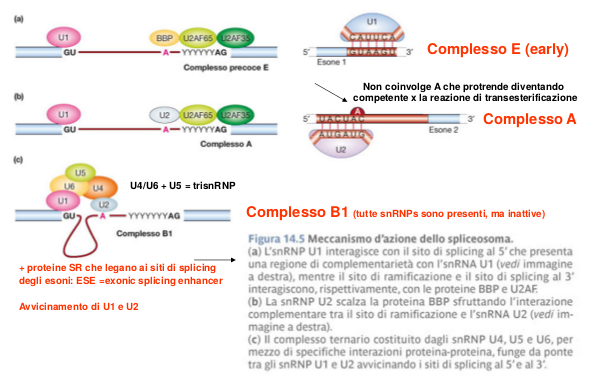
\includegraphics[scale=1.00]{img/46_Complessi E, A e B1 splicing.png}
\caption{}
\label{complessi-e-a-e-b1-splicing}
\end{figure}

A questo punto viene rilasciata la snRNP U1, che viene rimpiazzata dalla
\textbf{snRNP U6} nell'interazione complementare con il sito di splicing
al 5'. Questo è il \textbf{complesso B2}

Lo scambio tra U1 e U6 richiede la proteina \textbf{Prp8}, localizzata
nella \textbf{snRNP U5}, insieme ad ATP. Successivamente viene
rilasciata anche la snRNP U4, permettendo l'interazione tra le snRNP U2
e U6 dovuta alla complementarietà tra i due snRNA.

Lo spliceosoma così attivato (\textbf{complesso B}*) catalizza la prima
reazione di trans-esterificazione, nella quale viene idrolizzata una
molecola di ATP, formando il \textbf{complesso C1}.

Nel complesso C1 l'introne forma un intermedio a forma di cappio
(\emph{lariat}) che viene staccato dall'esone a valle nella seconda
reazione di trans-esterificazione, nella quale viene idrolizzata una
seconda molecola di ATP (\textbf{complesso C2}).

Infune, l'mRNA maturo viene rilasciato dallo spliceosoma che si dissocia
nelle snRNP componenti, che vengono riciclate.

\begin{figure}[htp]
\centering
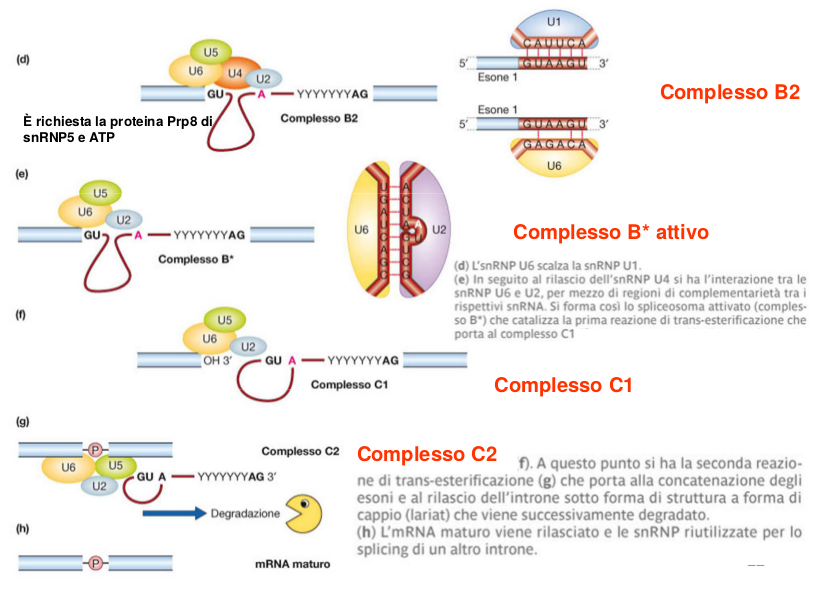
\includegraphics[scale=1.00]{img/47_Complesso B2, B*, C1 e C2 splicing.png}
\caption{}
\label{complesso-b2-b-c1-e-c2-splicing}
\end{figure}

Il meccanismo catalitico non è ancora chiaro; evidenze suggeriscono che
U2 e U6 contengono tutte le principali componenti del sito catalitico
utilizzando Prp8 come cofattore.

snRNP U2 e snRNP U6 hanno somiglianze strutturali con gli introni di
tipo II capaci di autosplicing (evoluzione dello splicing moderno).

L'mRNA matura non è nudo, ma associato a divers eproteine specifiche,
denominate \textbf{mRNP}, che svolgono un ruolo nel controllo
dell'accuratezza dello splicing dell'mRNA, facilitano il trasporto dal
nucleo al citoplasma e aumentano l'efficienza della traduzione.

In particolare, alcune proteine che costituiscono il \textbf{complesso
EJC} si legano all'mRNA neoformato a circa 24 nt a monte delle giunzioni
esone-esone, marcando così nell'mRNA maturo tutti i siti di splicing.

\subsection{Meccanismi per la corretta selezione dei siti di
splicing}\label{meccanismi-per-la-corretta-selezione-dei-siti-di-splicing}

Durante la selezione dei siti di splicing possono essere commessi degli
errori.

Vi sono due modi diversi per minimizzare gli errori:

\begin{itemize}
\itemsep1pt\parskip0pt\parsep0pt
\item
  man mano che la trascrizione procede i siti di splicing vengono
  caricati di specifiche componenti proteiche dalla coda CTD della
  polimerasi, in questo modo un sito 3' a valle di un sito 5' viene
  riconosciuto prima che gli altri competitori siano sintetizzati;
\item
  gli esoni vengono marcati dalle proteine SR (Ser+Arg) che si legano
  agli ESE (exonic splicing enhancers) e reclutano alcune componenti del
  macchinario di splicing.
\end{itemize}

\subsection{Trans-splicing}\label{trans-splicing}

Le reazioni di splicing fino ad ora descritte sono reazioni
\emph{intramolecolare} che producono la concatenazione di due esoni
presenti nella stessa molecola di RNA precursore
(\textbf{cis-splicing}).

Tuttavia lo splicing può aver luogo anche in trans quando le reazioni di
trans-esterificazione sono intermolecolari e portano alla concatenazione
di esoni provenienti da molecole differenti di RNA
(\textbf{trans-splicing}).

Il tipo più comune di trans-splicing consiste nel trasferimento di un
piccolo RNA non-codificante denominato \textbf{Sliced Leader (SL)},
proveniente da un RNA donatore (SL RNA) contenuto in una snRNP,
all'esone 5' terminale di un'altra molecola di RNA, trascritta
indipendentemente.

Il trans-splicing adotta un meccanismo identico a quello per lo splicing
nucleare e quindi richiede l'attività dello spliceosoma.

La differenza sostanziale sta nel fatto che il sito donatore (GU) e il
sito accettore (AG) sono su due diverse molecole di RNA, con il sito di
ramificazione e l'elemento ricco di pirimidine sull'RNA contenente il
sito accettore.

\begin{figure}[htp]
\centering
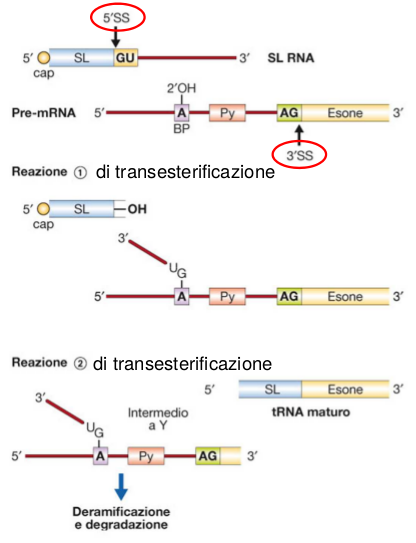
\includegraphics[scale=1.00]{img/48_Trans-splicing.png}
\caption{}
\label{trans-splicing}
\end{figure}

L'SL RNA è dotato di un cap e di un sito di splicing donatore (5'SS). Il
pre-mRNA contiene una adenina al sito di ramificazione un tratto di
poli-pirimidine (Py) e un sito accettore al 3' (3'SS). Nella prima
reazione di trans-esterificazione il 2'OH dell'adenina nel BP effettua
un attacco effettua un attacco nucleofilo sul fosfato al 5'SS. Nella
seconda trans-esterificazione l'attacco nucleofilo coinvogle il 3'OH
dell'RNA SL e il fosfato al 3'SS. In questo modo si forma l'mRNA maturo
dotato di un SL RNA al 5' con la liberazione di un RNA ramificato a
forma di Y che viene rapidamente degradato.

\subsection{Autosplicing}\label{autosplicing}

Nel 1982 alcuni scienziati scoprirono che un introne dell'rRNA di un
protozoo ciliato era capaci di autosplicing senza l'intervento di
fattori proteici.

Questi RNA possedevano dunque proprietà catalitiche e potevano svolgere
anche la funzione di un enzima (riboenzima).

Questi introni sono stati raggruppati in due classi distinte e
denominati \textbf{introni autocatalitici di classe I e II}, in funzione
del meccanismo catalitico utilizzato nella reazione di splicing.

Gli introni capaci di self-splicing hanno una lunghezza compresa tra 400
e 1000 nt e presentano una estesa conservazione sia nella sequenza che
nella struttura secondaria.

I meccanismi di autosplicing di questi 2 gruppi utilizzano due reazioni
di trans-esterificazione, ma con una differenza sostanziale: mentre
negli introni di tipo II la prima trans-esterificazione è effettuata,
analogamente al processo di splicing nucleare catalizzato dallo
spliceosoma, da 2'OH di una adenina interna all'introne stesso, negli
introni di tipo I essa è effettuata dal 3'OH di una guanosina esterna
alla sequenza dell'RNA.

\begin{itemize}
\itemsep1pt\parskip0pt\parsep0pt
\item
  \textbf{Introni del gruppo I}
\end{itemize}

Questi introni si torvano nei geni degli rRNA nucleari di alcuni
protozoi, e hanno dimensioni comprese tra 250 e 500 nt.

Contengono una ``tasca'' in grado di legare qualunque nucleotide o
nucleoside purchè contenga il ribosio. Inoltre hanno una
\textbf{sequenza guida interna} che si appaia alla sequenza del sito al
5' e determina il sito di attacco nucleofilo al P dell'introne 5'.

Questi introni assumono una struttura secondaria conservata che consiste
in diverse regioni appaiate, numerate da P1 a P9. A livello
tridimensionale questa struttura è organizzata in modo da avvicinare i
siti di splicing al 5' e al 3' ed è dotata delle attività catalitiche
necessarie per le due reazioni di trans-esterificzione.

Il meccanismo di splicing comporta due reazioni di
trans-esterificazione, la prima delle quali effettuata da una
\textbf{guanosina} esogena mono-, di- o trifosfato (\textbf{exoG}) il
cui 3'OH effettua un attaco nucleofilo al fosfato al 5' dell'introne. In
questa reazione l'exoG viene legata all'estremità 5' dell'introne
liberando il 3'OH dell'esone a monte. A questo punto una guanosina
all'estremità 3' dell'introne si colloca nel sito attivo, sclazando
l'exoG, dove ha luogo la seconda reazione di trans-esterificazione tra
il 3'OH dell'esone a monte e il fosfato del sito di splicing al 3'.

\begin{figure}[htp]
\centering
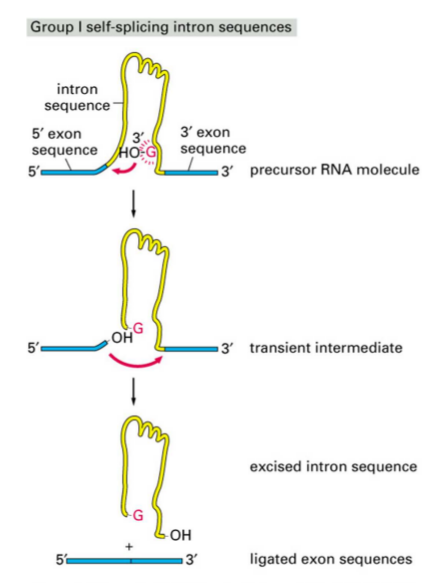
\includegraphics[scale=1.00]{img/49_Introni di gruppo I.png}
\caption{}
\label{introni-di-gruppo-i}
\end{figure}

\begin{itemize}
\itemsep1pt\parskip0pt\parsep0pt
\item
  \textbf{Introni del gruppo II}
\end{itemize}

Gli introni di questo gruppo hanno una lunghezza compresa tra i 400 e i
1000 nt.

La maggior parte degli introni del gruppo II è formata da due componenti
principali: un ribozima in grado di catalizzare la reazione di
autosplicing e una open reading frame codificante per proteine coinvolte
nello splicing e nella mobilizzazione dell'introne.

Questi introni sono caratterizzati da una struttura secondaria
conservata dotata di attività catalitica. La struttura secondaria del
ribozima è caratterizzata da sei tipiche strutture a stem-loop,
denominate D1-D6, che si irradiano da un nucleo centrale e si
organizzano a livello tridimensionale in modo da portare in prossimità i
siti di splicing al 5' e al 3'.

Il meccanismo catalitico è analogo a quello degli introni spliceosomali
e consiste di due reazioni di trans-esterificazione: la prima è data
dall'attacco nucleofilo del 2'OH di un'\textbf{adenina} interna
all'introne (nella regione D6) al fosfato del sito di splicing al 5'
nella seconda il 3'OH dell'esone a monte effettua un attacco nucleofilo
al fosfato nel sito di splicing al 3', risultante nella concatenazione
degli esoni e nella formazione di un intermedio a forma di cappio

\begin{figure}[htp]
\centering
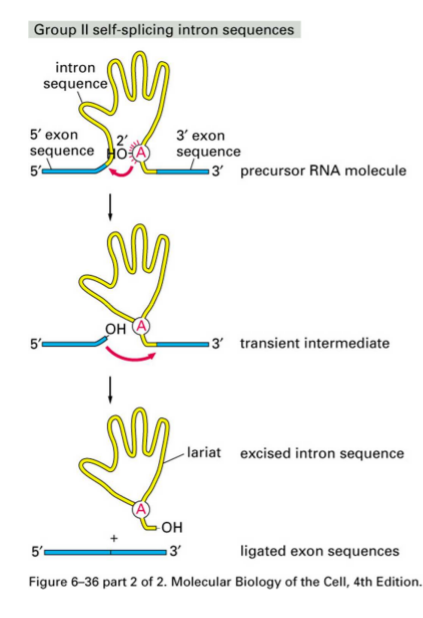
\includegraphics[scale=1.00]{img/50_Introni di gruppo II.png}
\caption{}
\label{introni-di-gruppo-ii}
\end{figure}

SnRNP U2 e snRNP U6 hanno somiglianze strutturali con gli introni di
tipo II. Forse il self-splicing del gruppo II è stato il punto di
partenza per l'evoluzione allo splicing tramite l'utilizzo dello
spliceosoma.

\subsection{Splicing alternativo}\label{splicing-alternativo}

Lo splicing alternativo consiste nel meccanismo attraverso il quale uno
stesso per-mRNA può subire eventi di splicing differenti che portano
alla creazione di diversi mRNA alternativi, che a loro volta possono
codificare differenti proteine.

Oltre il 90\% dei geni umani è interessato da splicing alternativo.

Questo fenomeno fu scoperto da Daved Baltimore che osservò che il gene
per la catena pesante \(\mu\) dell'immunoglobulina di topo poteva
esprimere una forma secreta (\(\mu\)\(_s\)) e una forma legata alla
membrana (\(\mu\)\(_m\)).

L'assortimento combinatorio di eventi di splicing può portare alla
generazione di un numero incredibilmente grande di trascritti, come nel
caso del gene \emph{Dscam} di Drosophila che può generare oltre 38000
varianti.

Il gene Dscam codifica per recettori che servono per la formazione di
connessioni neuronali, e sono caratterizzati da domini extracellulari
simili alle immunoglobuline uniti da una regione che attraversa la
membrana.

Questo gene ha 95 esoni variabili su 115 totali. L'mRNA maturo presenta
24 esoni, 4 dei quali (A, B, C e D), sono presenti come serie di esoni
alternativi. L'mRNA maturo contiene 1/12 alternative dell'esone A, 1/48
alternative dell'esone B, 1/33 alternative dell'esone C e 1/2
alternative dell'esone D. Tutte le combinazioni possibili (12 x 48 x 33
x 2) danno origine a 38016 trascritti alternativi codificanti proteine
che avrebbero la stessa struttura, ma con una sequenza aa diversa dei
domini A, B, C e D. NB: Drosophila ha circa 14000 geni!

\begin{itemize}
\item
  Un \textbf{esone costitutivo} è presente in tutte le varianti
  trascrizionali.
\item
  Un \textbf{esone regolato} è un esone alternativo che viene
  incorporato in funzione di segnali di regolazione.
\end{itemize}

Lo splicing alternativo può essere:

\begin{itemize}
\itemsep1pt\parskip0pt\parsep0pt
\item
  \textbf{costitutivo}. Se vi sono delle ambiguità nella sequenza
  intronica; il sistema non è in grado di distinguere tra 2 o più
  accoppiamenti alternativi. Tramite scelte \emph{casuali} vengono
  formate diverse versioni della proteina, e queste vengono prodotte in
  tutte le cellule in cui il gene viene espresso.
\end{itemize}

Un esempio è la trascrizione del gene \emph{CaMKII\(\delta\)}. Questo
gene contiene 3 esoni alternativi presenti in modo alternativo. Il gene
è espresso in tutti i tipi cellulari e tessuti di mammifero e codifica
per una chinasi. Le 3 isoforme svolgono la stessa attività ma hanno una
diversa localizzazione: \(\delta\)A si trova a livello neuronale, mentre
\(\delta\)B e \(\delta\)C si trovano a livello cardiaco.

\begin{itemize}
\itemsep1pt\parskip0pt\parsep0pt
\item
  \textbf{regolato}. Vengono prodotte versioni diverse della proteina in
  momenti, condizioni e tipi cellulari diversi (nella sua forma più
  semplice la proteina può essere semplicemente inattiva o attiva).
\end{itemize}

Un esempio è l'\(alpha\)-tropomionina di ratto regola la contrazione
delle cellule muscolari. Il pre-mRNA subisce schemi di splicing diversi
a seconda del tipo cellulare in cui viene trascritto.

\subsection{Regolazione dello
splicing}\label{regolazione-dello-splicing}

L'elevata specificità del riconoscimento dei siti di splicing dipende da
motivi di sequenza addizionali, coinvolti nella regolazione dello
splicing, e localizzati negli esoni o negli intorni, che agiscono come
\textbf{attivatori (enhancer)} o \textbf{repressori (silencer)} del
processo di splicing. Questi elementi di regolazione, in funzione della
loro localizzazione all'interno del pre-mRNA e della loro attività,
vengono classificati come \textbf{enhancer} e \textbf{silencer esonici
(ESE e ESS)} o \textbf{enhnacer} e \textbf{silencer intronici (ISE e
ISS)}.

Il prosesoo di splicing può essere controllato tramite un
\emph{controllo positivo} o \emph{negativo}.

Nel controllo positivo gli elementi ESE vengono normalmente riconosciuti
da proteine della famiglia \textbf{SR} che contengono uno o più domini
in grado di legare l'RNA e una regione, detta SR, ricca di serine e
arginine. L'interazione tra ESE e proteine SR facilita l'assemblaggio
dello spliceosoma.

Nel controllo negativo gli elementi ESS vengono, invece, legati da
repressori dello splicing, costituiti da una famiglia di
ribonucleoproteine denominate \textbf{hnRNP} contenenti domini
\textbf{RRM} capaci di legare l'RNA. L'interazione tra i motivi ESS e le
proteine hnRNP può inibire lo splicing attraverso vari meccanismi, che
tipicamento consistono nella inibizione di interazioni essenziali tra le
componenti dello spliceosoma o nel mascheramento degli stessi siti di
splicing.

Uno dei sistemi più studiati di regolazione dello splicing riguarda la
determinazione del sesso in \emph{Drosophila melanogaster}.

In \emph{Drosophila} il sesso è determinato dal rapporto tra i cromosomi
X e gli autosomi, pari a 1 nella femmina e a 0,5 nel maschio. Il
differente dosaggio del cromosoma X nei maschi e nelle femmine comporta
un diverso livello di espressione di due geni docificnati i
\emph{fattori trascrizionali} \textbf{SisA} e \textbf{SisB}, localizzati
sul cromosoma X doppio nelle femmina rispetto al maschio.

Questi fattori trascrizionali attivano l'espressione del gene denominato
\textbf{Sex-lethal (Sxl)} a partire da un suo \emph{promotore precoce}
(\textbf{P\(_e\)}).

L'azione di questi attivatori trascrizionali (\emph{SisA} e \emph{SisB})
è contrastata da un repressore trascrizionale codificato dal gene
\textbf{Dpn} e localizzato sul cromosoma 2.

Il gene \emph{Sxl} risulterà espresso solo nelle femmine, dove gli
attivatori espressi da \emph{SisA} e \emph{SisB} sono in eccesso
rispetto al prodotto \emph{dpn}.

Al contrario, nei maschi, in cui il livello di \emph{SisA} e \emph{SisB}
è dimezzato, prevarrà l'effetto del repressore \emph{Dpn} e \emph{Sxl}
non verrà espresso.

\emph{Sxl} viene poi trascritto, sia nelle femmine che nei maschi, a
partire da un secondo promotore denominato \textbf{P\(_m\)} (o di
mantenimento) a monte di \emph{P\(_e\)}. Il pre-mRNA così generato
subirà un diverso processo di splicing nei maschi e nelle femmine,in
quanto in queste ultime \emph{Sxl}, già presente perchè espressa a
partire da \emph{P\(_e\)}, è in grado di autoregolare lo splicing del
suo pre-mRNA.

\emph{Sxl} funge da \textbf{repressore} dello splicing inducendo
l'espressione di due isoforme di mRNA \emph{Sxl}, di cui solo quella
espressa nelle femmine è in grado di esprimere una proteina funzionale,
che a sua volta controlla lo splicing del gene \textbf{tra}
(transformer).

Solo l'isoforma di \emph{tra} espressa nelle femmine codifica per un
prodotto funzionale che a differenza di Sxl funziona come attivatore
dello splicing utilizzando come cofattore la proteina \emph{Tra2}. In
questo modo nei maschi e nelle femmine vengono prodotte due isoforme
differenti della proteina \emph{doublesex (dsx)}. Queste due isoforme
hanno una porzione N-terminale in comune e una porzione C-terminale
maschio-specifica (150 aa) o femmina-specifica (30 aa) che inducono lo
sviluppo dello stato maschile o femminile.

\textbf{(AGGIUNGERE???)}

\subsection{Editing dell'RNA}\label{editing-dellrna}

L'editing dell'RNA è un processo post-trascrizionale che genera molecole
di RNA che differiscono dal loro stampo di DNA in una o più posizioni,
modificando così l'informazione genetica presente nel gene. L'editing
utilizza due diversi meccanismi:

\begin{itemize}
\itemsep1pt\parskip0pt\parsep0pt
\item
  la \textbf{conversione} di una base in un'altra;
\item
  l'\textbf{inserzione} o \textbf{delezione} di nucleotidi.
\end{itemize}

La funzione svolta dall'editing è quella di apportare le opportune
correzioni per rendere i trascritti funzionali o per modulare
l'espressione di prodotti alternativi in diverse condizioni o tessuti.

Esempi di editing per conversione di basi nei mammiferi sono:

\begin{itemize}
\itemsep1pt\parskip0pt\parsep0pt
\item
  la conversione della citosina in uracile nel gene per
  l'\textbf{apolipoproteina B}, il cui trascritto a seconda che subisca
  o meno il processo di editing, può codificare due proteine distinte
  \textbf{ApoB100} e \textbf{ApoB48}.
\end{itemize}

\textbf{ApoB100} viene prodotta negli epatociti del fegato e serve per
il trasporto e il rilascio del colesterolo ai tessuti, mentre
\textbf{ApoB48} viene prodotta nell'intestino e serve per il trasporto
del colesterolo ai tessuti.

La conversione della citosina in uracile nella posizione 6666 dell'mRNA,
catalizzata dalla deaminasi APOBEC1, avviene solo nell;intestino e,
comportando la trasformazione del codone CAA in UAA, introduce un codone
di stop prematuro, responsabile della formazione dell'isoforma ApoB.

\begin{itemize}
\itemsep1pt\parskip0pt\parsep0pt
\item
  la conversione di adenosina (A) in inosina (I). Questo evento
  interessa il gene per la subunità 2 del canale ionico AMPA che
  risponde al glutammato (GRIA2) in cui uno degli enzimi ADAR riconosce
  come substrato l'RNA a doppio filamento formato dall'appaiamento di un
  esone e del successivo introne (l'editing avviene prima dello
  splicing). L'editing in GRIA2 introduce cambiamenti nella sequenza
  amminoacidica.
\end{itemize}

La conversione della glutamina in arginina modifica la permeabilità al
calcio del canale. Senza questo editing sia lo sviluppo del cervello che
del sistema ematopoietico sono gravemente compromessi.

Un esempio di editing inserzionale è stato scoperto nel protozoo
\emph{Trypanosoma brucei}.

L'RNA prodotto da questi protozoi diviene funzionale solo dopo che
l'editing, che consiste nell'aggiunta e delezione di uridine in
specifiche posizioni, sia stato completato.

I geni sono quindipresenti nel genoma in una forma criptica e sono
ufficialmente riconoscibili. Per questa ragione sono anche definiti
\textbf{criptogeni}. Le posizioni specifiche che dovranno essere editate
e il numero corretto di U sono determinati dagli \textbf{RNA guida
(gRNA)}. Questi sono piccoli RNA che contengono una breve sequenza
antisenso che si appaia con il trascritto non editato a valle del sito
in cui andranno inserite o eventualmente rimosse le uridine.

Nell'editing per inserzione di nucleotidi, nella zona adiacente al
tratto di complementarietà si ha una regione (regione di editing) non
appaiata per la presenza di A che non hanno le corrispettive U nel
pre-mRNA. Una endonucleasi taglia in corrispondenza del sito di editing
riconoscendo la regione non appaiata con i gRNA e, successivamente,
l'enzima \textbf{TUTasi (Terminal Uridil Transferasi)} aggiunge le U al
3'OH del frammento di pre-RNA a monte. Una ligasi, infine, unisce le
estremità 3'OH e 5'-fosfato ristabilendo la continuità della molecola di
RNA.

Il processo di editing inserzionale è generalmente molto esteso e
richiede numerosi gRNA.

Le molecole di \emph{gRNA} presentano 3 regioni:

\begin{enumerate}
\def\labelenumi{\arabic{enumi}.}
\itemsep1pt\parskip0pt\parsep0pt
\item
  una regione \textbf{ancora};
\item
  una regione indicante il sito di aggiunta di U (ricca in A);
\item
  un segmento 3' poli-U il cui ruolo non è chiaro.
\end{enumerate}

Procedimento:

\begin{itemize}
\itemsep1pt\parskip0pt\parsep0pt
\item
  la regione ancora si appaia a valle della regione da editare;
\item
  la regione ricca in A del gRNA protrude poichè non presenta basi
  complementari sul pre-RNA;
\item
  un'endonucleasi riconosce questa struttura e taglia sul filamento
  opposto (RNA da editare);
\item
  una TUTasi addiziona le U;
\item
  una RNA ligasi ricollega il filamento.
\end{itemize}

\subsection{Traslocazione nucleo-citoplasmatica degli
RNA}\label{traslocazione-nucleo-citoplasmatica-degli-rna}

Una volta completato il processo di maturazione all'interno del nucleo
gli RNA devono essere traslocati nel citoplasma, dove l'mRNA maturo pfà
essere tradotto in proteina.

Il trasporto di molecole con PM superiore ai 50kDa avviene tramite un
processo di trasporto attivo (richiede energia) mediato dal
\textbf{complesso del poro nucleare (NPC)}, grandi complessi
multiproteici i cui componenti sono denominati \textbf{nucleoporine}.

I fattori proteici che agiscono come mediatori del trasporto attivo
degli mRNA attraversp gli NPC controllano anche che il processo di
maturazione sia stato completato e sia avvenuto correttamente. Solo le
molecole di mRNA associate al giusto corredo di proteine dunque, sono
selezionate per il trasporto; questo passaggio viene chiamato
\textbf{rimodellamento dell'mRNP}.

Il trasporto è mediato dai recettori di trasporto nucleare che vengono
caricati sull'mRNA maturo. Una volta trasportato nel citoplasma il
recettore di trasporto nucleare si stacca e ritorna nel nucleo per
essere riciclato.

\section{La traduzione}\label{la-traduzione}

\subsection{Il codice genetico}\label{il-codice-genetico}

Il codice genetico è lo stesso in tutti gli organismi, procarioti ed
eucarioti, per cui viene detto che il \emph{codice genetico è}
\textbf{universale}.

Il codice genetico è formato da 64 codoni (triplette di basi), 3 dei
quali (\textbf{UAA}, \textbf{UAG} e \textbf{UGA}) non codificano per
alcun amminoacido, e sono detti \textbf{codoni di stop}. I codoni di
stop segnalano la terminazione della sintesi proteica.

Gli altri 61 codoni codificano per i 20 tipi di amminoacidi che vengono
utilizzati nella sintesi proteica: ne deriva che un amminoacido può
essere codificato da più codoni. I diversi codoni che specificano per lo
stesso amminoacido vengono chiamati \textbf{codoni sinonimi} e un codice
così fatto viene detto \textbf{codice degenerato}.

Il codice genetico però \emph{non è ambiguo}, cioè ciascum codone
codifica per un solo amminoacido, senza eccezioni.

Il protagonista della sintesi proteica è l'RNA:

\begin{itemize}
\itemsep1pt\parskip0pt\parsep0pt
\item
  l'\textbf{RNA messaggero (mRNA)} porta l'informazione copiata dal DNA
  sotto forma di codoni;
\item
  l'\textbf{RNA transfer (tRNA)} decifra il codice mediante uno
  specifico anticodone e, associato a lui vi è un particolare
  amminoacido;
\item
  l'\textbf{RNA ribosomale (rRNA)} si associa con una serie di proteine
  per formare iribosomi, per sintetizzare le proteine.
\end{itemize}

\subsection{Il tRNA}\label{il-trna}

Francis Crick ipotizzò l'esistenza di ``adattatori'' molecolari che
potessero riconoscere da una parte i codoni del messaggio genetico e
dall'altra gli specifici amminoacidi da inserire nella sequenza delle
proteine. Questo adattatore è il \textbf{tRNA (RNA transfer, RNA di
trasferimento)}. In ogni cellula esiste almeno un tipo di tRNA per
ciascuno dei 20 tipi di amminoacidi utilizzati nella sintesi proteica,
ma spesso ve ne è anche più di uno.

I tRNA sono piccole molecole costituite da una sequenza di 73-93 nt. I
tRNA hanno una caratteristica struttura secondaria a trifoglio
risultante dall'appaiamento di basi complementari che si trovano in
diverse regioni della sequenza nucleotidica.

Nella struttura a trifoglio riconosciamo:

\begin{itemize}
\itemsep1pt\parskip0pt\parsep0pt
\item
  un \textbf{braccio accettore} formato dalle due estremità della
  molecola;
\item
  3 bracci costituiti ciascuno da uno stelo a doppio filamento e da
  un'ansa di basi non appaiate, chiamato \textbf{braccio T\(\Psi\)C};
\item
  un \textbf{braccio D};
\item
  un \textbf{braccio dell'anticodone}
\item
  un braccio accessorio di lunghezza variabile (a volte).
\end{itemize}

Il \textbf{braccio accettore} è formato dall'appaiamento delle due
estremità della molecola, ed è così chiamato perchè su di esso si lega
l'amminoacido. L'amminoacido si lega all'estremità 3', che è sempre una
A preceduta da due C.

Il \textbf{braccio T\(\Psi\)C} così chiamato per la presenza, nella sua
ansa a singolo filamento, di questa sequenza, dove T indica una timina e
\(\Psi\) indica la base modificata \textbf{pseudouridina}.

Il \textbf{braccio D} prende il nome dalla presenza nella sua ansa di
un'altra base modificata, la \textbf{diidrouridina}.

Il \textbf{braccio dell'anticodone} è così chiamato per la presenza
nella sua ansa della tripletta di nucleotidi che riconosce per
appaiamento di basi il codone sull'mRNA, e si trova sempre fiancheggiata
al lato 3' da una purina e al lato 5' da un uracile.

Il \textbf{braccio variabile} è situato tra il braccio T\(\Psi\)C e
quello dell'anticodone ed è di lunghezza variabile da 3 a 21 basi nei
diversi tRNA.

La struttura a trifoglio non rappresenta la vera struttura dei tRNA. I 4
steli a doppio filamento infatti, vanno nel loro insieme a formare una
struttura tridimensionale complessa. La struttura secondaria a trifoglio
di tutti i tRNA è ripiegata su se stessa a formare una struttura
terziaria (tridimensionale) a \textbf{L}.

Nella struttura a L troviamo l'anticodone all'estremità del braccio
lungo della L, questo è esposto verso l'esterno per rotazione della
regione dell'anticodone. L'amminoacido è caricato sull'estremità del
braccio corto della L. I due bracci T\(\Psi\)C e D vanno a formare
l'angolo della L, con le due anse non appaiate all'esterno dell'angolo.

\begin{figure}[htp]
\centering
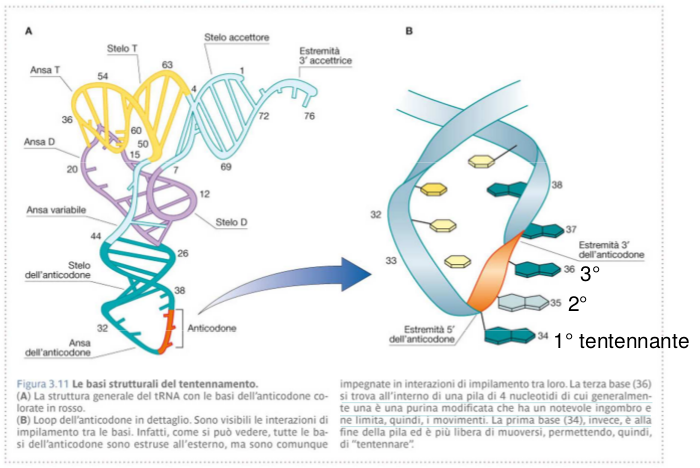
\includegraphics[scale=1.00]{img/51_Struttura L del tRNA.png}
\caption{}
\label{struttura-l-del-trna}
\end{figure}

I tRNA vengono trascritti sotto forma di precursori che dovranno subire
un processo di maturazione per generare i tRNA funzionali.

I pre-tRNA eucariotici e procariotici contengono estremità più estese
sia al 5' che al 3' che dovranno essere rimosse dall'azione di
endonucleasi ed esonucleasi per generare le molecole di tRNA mature e
funzionali. L'estremità 5' del tRNA maturo viene generata d aun taglio
endonucleolitico catalizzato dall'enzima \textbf{RNasi P}, una
ribonucleoproteina la cui componente primaria è l'\textbf{RNA M1} che
esercita l'attività catalitica.

I tRNA non hanno però alcuna diretta affinità specifica per gli
amminoacidi che devono caricare. Il processo di caricamento degli
amminoacidi sui corrispondenti tRNA viene catalizzato da una classe di
enzimi, chiamati \textbf{amminoacil-tRNA sintetasi}.

Mentre ogni amminoacil-tRNA sintetasi riconosce specificamento un solo
amminoacido, essa riconosce tuti i tRNA sui quali questo può essere
caricato, cioè i cosiddetti \textbf{tRNA isoaccettori}.

Il ruolo delle amminoacil-tRNA sintetasi è quello di catalizzare la
formazione di un legame acilico ad alta energia tra il gruppo
carbossilico dell'amminoacido e il gruppo idrossilico in posizione 2' o
3' della adenosina che costituisce l'estremità 3' del tRNA.

Il caricamento dell'amminoacido sul tRNA avviene in due passaggi
consecutivi, entrambi catalizzati dalla stessa amminoacil-tRNA
sintetasi:

\begin{enumerate}
\def\labelenumi{\arabic{enumi}.}
\itemsep1pt\parskip0pt\parsep0pt
\item
  l'amminoacido viene attivato usando l'energia di una moleocla di ATP
  formando amminoacil-AMP (aa) e rilasciando pirofosfato (PP\(_1\));
\end{enumerate}

\begin{figure}[htp]
\centering
\includegraphics[scale=1.00]{img/52_Attivazione tRNA (1).png}
\caption{}
\label{attivazione-trna-1}
\end{figure}

\begin{enumerate}
\def\labelenumi{\arabic{enumi}.}
\setcounter{enumi}{1}
\itemsep1pt\parskip0pt\parsep0pt
\item
  l'energia dell'amminoacil-AMP viene utilizzata per trasferire
  l'amminoacido al tRNA per formare amminoacil-tRNA con liberazione di
  AMP.
\end{enumerate}

\begin{figure}[htp]
\centering
\includegraphics[scale=1.00]{img/53_Attivazione tRNA (2).png}
\caption{}
\label{attivazione-trna-2}
\end{figure}

Le amminoacil-tRNA sintetasi hanno sempre 3 siti di legame:

\begin{enumerate}
\def\labelenumi{\arabic{enumi}.}
\itemsep1pt\parskip0pt\parsep0pt
\item
  uno per l'amminoacido;
\item
  uno per il tRNA corrispondente;
\item
  uno per la molecola di ATP necessaria alla reazione.
\end{enumerate}

Le amminoacil-tRNA sintetasi possono essere monomeriche, dimeriche o
tetrameriche, ma svolgono sempre la stessa funzione. Sulla base della
struttura del loro sito attivo, le sintetasi possono essere divise in
due gruppi:

\begin{enumerate}
\def\labelenumi{\arabic{enumi}.}
\itemsep1pt\parskip0pt\parsep0pt
\item
  le \textbf{sintetasi di classe I}, generalmente monomeriche, legano
  inizialmente l'amminoacido al 2'OH del tRNA; 2.le \textbf{sintetasi di
  classe II}, generalmente dimeriche o tetrameriche, legano
  l'amminoacido al 3'OH del tRNA.
\end{enumerate}

Esistono dei meccanismi di controllo dell'accuratezza del caricamento
dei tRNA; questo meccanismo viene detto di \textbf{``correzione di
bozze''}. In genere le sintetasi escludono dal sito di attivazione
alcuni amminoacidi perchè troppo grandi o con forme diverse da quella
corretta, ma possono erroneamente accettare un amminoacido errato
strutturalemnte simile a quello corretto.

La frequenza di errore viene ridotta dal passaggio dell'amminoacil-AMP,
prima del trasferimento sul tRNA, in un \emph{``sito di correzione''}
presente nell'enzima stesso.

\textbf{Esempio:} amminoacil-sintetasi per l'isoleucina di \emph{E.
coli}.

Questa sintasi esclude dal sito alcuni amminoacidi perchè
strutturalmente troppo grandi o non compatibili, ma può accettarne altre
sempre non corrette, come la \emph{valina} e attivarla (cioè legarla
all'AMP. L'amminoacido attivato però, prima di essere trasferito sul
tRNA, transita nel sito di correzione dell'enzima stesso che, se
l'amminoacido è corretto (in questo caso l'isoleucina), lascia prosegure
la reazione, mentre se coinvolge un amminoacido errato (come la valina)
porta a idrolisi del \emph{Val-AMP}.

La frequenza con cui la valina viene caricata erroneamente sull'AMP è di
1/225, mentre la frequenza con cui il meccanismo di correzione fallisce
è di 1/270. Questo significa che la frequenza con cui viene formato
Val-tRNA\(^I\)\(^l\)\(^e\) è di: (1/225 x 1/270) = 1/60.000

\begin{itemize}
\itemsep1pt\parskip0pt\parsep0pt
\item
  \textbf{La teoria del vacillamento}
\end{itemize}

Poiché il codice genetico utilizza 61 codoni diversi per specificare 20
amminoacidi, ci si aspetta che nella sintesi proteica siano coinvolti 61
diversi tRNA, di cui alcuni caricati con lo stesso amminoacido. Tuttavia
molti tRNA riconoscono più di un codone, facendo sì che il numero dei
tRNA totali sia molto inferiore a 61 (es. nell'uomo sono presenti solo
48 tRNA diversi).

La degenerazione del codice genetico in terza posizione (uno stesso
amminoacido può essere espresso da più triplette che differiscono solo
per la terza base), suggerì che nel riconoscimento codone-anticodone
fossero implicati solo due appaiamenti di basi (1a e 2a del codone, 3a e
2a dell'anticodone). Non ci sarebbe un appaiamento specifico tra la 3a
base del codone e la 1a dell'anticodone.

Crick propose la \textbf{teoria del vacillamento (wobble)}, per cui
nell'appaiamento codone-anticodone nel sito di decodificazione del
ribosoma, l'ansa dell'anticodone del tRNA presenta una certa
deformazione strutturale conferendo al tRNA una certa flessibilità di
appaiamento.

Inoltre, nella posizion 1 dell'anticodone, possono essere presenti basi
modificate quali l'inosina e la tiouridina che hanno proprietà di
appaiamento delle basi particolari.

\subsection{Il ribosoma}\label{il-ribosoma}

I ribosomi sono delle \emph{``macchine molecolari''} che sintetizzano le
proteine decodificando l'informazione portata dall'mRNA.

Tutti i ribosomi, sia procariotici che eucariotici, sono delle
particelle ribonucleoproteiche, cioè sono composti da alcune molecole di
RNA (\textbf{rRNA}) e da numerose proteine (\textbf{rp = proteine
ribosomali}),

rRNA e r-proteine sono assemblati a costituire due subunità ribosomali
distinte, una maggiore e una minore.

I ribosomi, le loro subunità e gli RNA che li compongono vengono
generalemnte denominati in base alla loro velocità di sedimentazione. I
valori in S delle subunità non sono additivi rispetto a quelli dei
ribosomi interi perchè la velocità di sedimentazione non è direttamente
proporzionale alla massa.

I ribosomi procariotici sono, nel loro intero, denominati \textbf{70S} e
sono formati da una subunità \textbf{30S} e da una \textbf{50S}. Quelli
eucarioti sono, nel loro insieme, denominati \textbf{80S} e sono formati
da una subunità \textbf{40S} e da una \textbf{60S}.

Se in una cellula si nota un'alta presenza di rRNA significa che vi sono
molti geni codificanti.

La sintesi e la maturazione degli rRNA avviene nel nucleolo (corpo
granulare sferico non delimitato da membrana). I geni codificanti per
gli rRNA vengono trascritti sotto forma di grandi molecole di RNA
precursore \textbf{pre-rRNA} che poi daranno origine alle molecole di
RNA mature in seguito all'escissione delle porzioni in eccesso. Questo
processo è denominato \textbf{processing (processamento)}.

Il processing consiste in una serie di tagli endonucleolitici ed
esonucleolitici 3'\(\rightarrow\) 5' e 5' \(\rightarrow\)-3', ma non si
ha la concatenazione dei frammenti prodotti (come avviene invece nello
splicing). Il processing incomincia quando la trascrizione è quasi
completata.

In \emph{E. coli} i geni per gli rRNA sono presenti in 7 copie,
organizzati in altrettanti operoni ciascuno dei quali contiene una copia
di ciascun tipo di rRNA (rRNA 5S, rRNA 16S, rRNA 23S).

La trascrizione dell'operone genera un RNA precursore 30S che poi subirà
un processing che richiede l'azione della \textbf{RNasi III}. Questo
enzima effettua tagli endonucleoltici in 2 regioni complementari che
fiancheggiano sia l'rRNA 16S che 23S.

I pre-rRNA separati sono processati dalla \textbf{RNasi E}
(endonucleasi, responsabile della rimozione dell'rRNA 5S dalla molecola
precursore) al 5', ed al 3' dalla esonucleasi \textbf{RNasi T}.

\begin{figure}[htp]
\centering
\includegraphics[scale=1.00]{img/54_Processing rRNA.png}
\caption{}
\label{processing-rrna}
\end{figure}

Il gene per l'rRNA 5S sono organizzati in tandem, hanno una diversa
localizzazione nel genoma, non sono trascritti nel nucleolo e sono
trascritti dalla RNA pol III. Viene processato per rimozione dei nt al
3'. Entra poi nel nucleolo.

Come snoRNP (ribonucleoproteine) gli RNA guida si appaiano a regioni
complementari del pre-rRNA e portano un enzima che modifica la posizione
appropriata. Altri RNA guida provocano modificazioni conformazionali
della struttura del pre-rRNA esponendo i siti di taglio alla nucleasi
per formare l'rRNA maturo. Tutti questi RNA sono snoRNA ed agiscono
insieme a proteine per formare le snoRNP (es. snoRNA E1 e E2 partecipano
alla maturazione del 18S e snoRNA E3 a quella del 5.8S).

Gli rRNA hanno una struttura secondaria complessa dovuta ad appaiamenti
di basi intramolecolari tra regioni complementari. Le regioni appaiate
assumono una struttura a doppia elica e nel loro insieme si ripiegano,
nel ribosoma, in una complessa struttura tridimensionale.

\begin{itemize}
\itemsep1pt\parskip0pt\parsep0pt
\item
  \textbf{La biogenesi dei ribosomi}
\end{itemize}

\begin{figure}[htp]
\centering
\includegraphics[scale=1.00]{img/55_Biogenesi ribosomi.png}
\caption{}
\label{biogenesi-ribosomi}
\end{figure}

La biogenesi dei ribosomi è stata studiata in S. cerevisiae; è un
processo dinamico che comprende la sintesi e la modificazione dell'rRNA,
l'assemblaggio con le r-proteine e l'assemblaggio transitorio con
proteine non rp.

Una volta avvenuto l'assemblaggio i ribosomi vengono trasportati
attraverso i pori nucleari nel citoplasma.

\begin{itemize}
\itemsep1pt\parskip0pt\parsep0pt
\item
  \textbf{La struttura del ribosoma}
\end{itemize}

La struttura complessiva dei ribosomi è dovuta soprattutto agli rRNA che
con la loro struttura tridimensionale costituiscono l'impalcatura su cui
si assemblano le rp. Le rp si trovano per lo più nella parte esterna del
ribosoma, e hanno in genere una struttura globulare con prolungamenti
che si infilano nell'rRNA.

Le rp (rpL e rpS) assistono l'rRNA nel ripiegamento e nell'acquisizione
della sua corretta struttura tridimensionale. Le rp sono in genere delle
proteine piccole e basiche che non partecipano direttamente alla
catalisi.

È possibile costituire subunità ribosomali funzionanti in vitro. Perchè
questo avvenga le r-proteine devono essere aggiunte all'rRNA in
\emph{gruppo con un ordine definito}.

In E. coli il primo passaggio della ricostituzione della subunità 30S è
l'associazione dell'rRNA 16S con un gruppo di 15 r-proteine, che sono le
ultime che si erano staccate al momento della dissociazione della
subunità ribosomale. Solo dopo si ha l'assemblaggio delle rimanenti 6
r-proteine (le prime che si erano dissociate). All'interno di questi
gruppi anche le singole r-proteine si associano alla ribonucleoproteina
in formazione con un ordine preciso: alcune si associano per prime
legandosi direttamente all'rRNA, mentre altre si possono associare solo
dopo che si sono assemblate le prime.

Nella struttura della subunità minore 30S distinguiamo una ``base'' e
una ``testa''; dalla base protrude una ``piattaforma'' che è separata
dalla testa da un ``solco''. Nella subunità maggiore 50S osserviamo una
``protuberanza centrale'' fiancheggiata da un lato da un ``peduncolo'' e
dall'altro da una ``cresta''. Quest'ultima è separata dalla protuberanza
centrale da una ``valle''.

\begin{figure}[htp]
\centering
\includegraphics[scale=1.00]{img/56_Ribosoma.png}
\caption{}
\label{ribosoma}
\end{figure}

Il ribosoma ha 3 siti di legame per il tRNA:

\begin{enumerate}
\def\labelenumi{\arabic{enumi}.}
\itemsep1pt\parskip0pt\parsep0pt
\item
  il \textbf{sito A} (accettore), che lega il tRNA amminoacilato in
  ingresso;
\item
  il \textbf{sito P} (peptidilico), che lega l'ultimo tRNA entrato e
  porta la catena peptidica nascente;
\item
  il \textbf{sito E} (exit), che lega il tRNA scarico che deve essere
  rilasciato.
\end{enumerate}

I siti A e P si trovano a cavallo tra le due subunità, cosicché ciascuno
di essi è composto di due emisiti, uno nella subunità minore e uno nella
subunità maggiore del ribosoma.

I tRNA sono posizionati in modo che gli anticodoni, che si torvano
all'estremo del braccio lungo della struttura a L dei tRNA, si possano
appaiare con i codsoni dell'mRNA nella subunità minore del ribosoma in
quello che viene chiamato \textbf{centro di decodificazione}. Le
estremità del braccio corto della struttura a L dei tRNA che portano
l'amminoacido e il peptide nascente, si trovano nella subunità maggiore
e in particolare nel \textbf{centro della peptidil transferasi}, sito
responsabile della formaizone dei legami peptidici.

Nella subunità 30S sono presenti due piccoli canali, uno di entrata e
uno di uscita, in cui scorre l'mRNA durante il processo di traduzione.

Il canale di entrata è di una larghezza tale per cui l'mRNA perde le sue
strutture secondarie ed entra disteso nel centro di deocdificazione,
dove gli appaiamenti codone-anticodone nei siti A e P sono facilitati
dal fatto che, tra i due codoni, l'mRNA forma un angolo. Nella subunità
50S si trova un altro canale, il tunnel per l'Fuscita della catena
peptidica nascente che attraversa la subunità partendo dal centro
peptidil transferasico.

\begin{figure}[htp]
\centering
\includegraphics[scale=1.00]{img/57_Siti ribosoma.jpg}
\caption{}
\label{siti-ribosoma}
\end{figure}

\section{I meccanismi della sintesi
proteica}\label{i-meccanismi-della-sintesi-proteica}

Sia nei procarioti che negli eucarioti la sintesi di tutte le proteine
inizia all'\emph{estremità ammino terminale} (segue la direzione
NH\(_2\)-terminale \(\rightarrow\) COOH-terminale) come l'amminoacido
\textbf{metionina}.

Questo aa è codificato dal codone \textbf{AUG} (in alcuni casi vengono
usati i codoni GUG e UUG).

La sintesi proteica si divide in 3 fasi: inizio, allungamento e
terminazione.

\subsection{L'inizio della sintesi nei
procarioti}\label{linizio-della-sintesi-nei-procarioti}

Nei procarioti la metionina di inizio è modificata chimicamente per
aggiunta di un \textbf{gruppo formilico} che ne blocca il gruppo
amminico. Questo avviene ad opera dell'enzima \textbf{metionil-tRNA
transformilasi} dopo essere stata caricata sul tRNA.

Il gruppo amminico degli aa, durante la sintesi proteica, è essenziale
per la formazione del legame peptidico con l'aa precedente. La presenza
del gruppo formilico impedisce perciò alla metionina modificata di
essere utilizzata nella fase di allungamento.

Per questo motivo nella cellula ci sono 2 tipo di tRNA per la metionina:

\begin{itemize}
\itemsep1pt\parskip0pt\parsep0pt
\item
  il tRNA di inizio \textbf{tRNA\(_i\)\(^f\)\(^M\)\(^e\)\(^t\)} per la
  metionina che verrà formilata;
\item
  il \textbf{tRNA\(^M\)\(^e\)\(^t\)} per le metionine che saranno
  inserite internamente alle catene peptidiche.
\end{itemize}

Inoltre il tRNA di inizio fMet-tRNA\(_i\)\(^f\)\(^M\)\(^e\)\(^t\) entra
direttamente nell'\emph{emisito P} senza passare nel sito A (come tutti
gli altri amminoacil-tRNA).

\begin{figure}[htp]
\centering
\includegraphics[scale=1.00]{img/59_tRNA di inizio.png}
\caption{}
\label{trna-di-inizio}
\end{figure}

L'inizio della traduzione convolge sempre l'interazione preliminare tra
la sub. minore del ribosoma, fMet-tRNA\(_i\)\(^f\)\(^M\)\(^e\)\(^t\), e
mRNA (formano sub. 30S). Solo successivamente viene richiamata la
subunità maggiore e si forma il complesso di inizio 70S.

È necessario che il complesso di inizio si assembli sull'mRNA in
corrispondenza del codone di inizio (in genere AUG). I codoni AUG
possono ovviamente essere presenti in più punti durante la fase di
lettura aperta (ORF) senza però avere la funzione di segnale di inizio
della traduzione.

Come viene selezionato un codone AUG di inizio?

Pochi nucleotidi a monte dell'AUG di inizio troviamo una sequenza molto
conservata che viene chiamata \textbf{sequenza di Shine-Dalgarno (SD o
RBS)}. Questa sequenza, AGGAGG, precede di 7 nucleotidi il codone di
inizio e rappresenta il sito di legame dei ribosomi all'mRNA.

Questa sequenza viene riconosciuta da una sequenza complementare di
pirimidine sull'rRNA 16S della subunità ribosomiale minore (30S).
L'interazione è fra estremità 3' dell'rRNA 16S con la sequenza di
Shine-Dalgarno (è sufficiente un appaiamento di 4-6 basi).

\begin{figure}[htp]
\centering
\includegraphics[scale=1.00]{img/58_Shine-Dalgarno.png}
\caption{}
\label{shine-dalgarno}
\end{figure}

\subsubsection{Fattori di inizio nei
procarioti}\label{fattori-di-inizio-nei-procarioti}

Per il processo di inizio sono necessari anche vari fattori proteici,
detti \textbf{fattori di inizio}, che nei procarioti sono solo 3:

\begin{itemize}
\itemsep1pt\parskip0pt\parsep0pt
\item
  \textbf{IF1}

  \begin{enumerate}
  \def\labelenumi{\arabic{enumi}.}
  \itemsep1pt\parskip0pt\parsep0pt
  \item
    contribuisce insieme a IF3 alla dissociazione del ribosoma 70S;
  \item
    si lega alla subunità 30S nella regione che andrà a formare il sito
    A del ribosoma impedendo agli amminoacil-tRNA di entrarvi;
  \end{enumerate}
\item
  \textbf{IF2} è una GTPasi (lega e idrolizza GTP per funzionare) che:

  \begin{enumerate}
  \def\labelenumi{\arabic{enumi}.}
  \itemsep1pt\parskip0pt\parsep0pt
  \item
    interagisce con la sub. 30S;
  \item
    promuove l'associazione con fMet-tRNA\(_i\)\(^f\)\(^M\)\(^e\)\(^t\)
    all'emisito P;
  \item
    impedisce l'interazione con altri tRNA carichi;
  \end{enumerate}
\item
  \textbf{IF3}

  \begin{enumerate}
  \def\labelenumi{\arabic{enumi}.}
  \itemsep1pt\parskip0pt\parsep0pt
  \item
    è coinvolto nella dissociazione dei ribosomi interi nelle due
    subunità;
  \item
    legato alla sub. 30S è essenziale perchè questa si leghi in modo
    specifico al sito di inizio sull'mRNA;
  \item
    impedisc eil precoce legame con la sub. 50S;
  \item
    aumenta la specificità del sito P per
    tRNA\(_i\)\(^f\)\(^M\)\(^e\)\(^t\).
  \end{enumerate}
\end{itemize}

Tutti e tre i fattori interagiscono con la subunità minore del ribosoma
e sono necessari per la formazione del complesso di inizio 30S.

\subsubsection{Processo di inizio della traduzione nei
procarioti}\label{processo-di-inizio-della-traduzione-nei-procarioti}

Si ha un primo intervento di IF1, che legandosi alla sub. 30S nel
ribosoma intero contribuisce alla dissociazione dello 2 sub.. IF3 invece
interagisce solo con la sub. 30S già dissociata e, impedendone la
riassociazione con la sub. 50S la mantiene disponibile per un nuovo
inizio.

A questo punto \textbf{IF2-GTP} va a legarsi alla subunità 30S in
prossimità dell'emisito P dove promuove l'ingresso del tRNA di inizio
fMet-tRNA\(_i\)\(^f\)\(^M\)\(^e\)\(^t\). A questo punto si ha il legame,
mediato da IF3, dell'mRNA alla sub. 30S.

Nel complesso di inizio 30S la presenza di IF1 e IF2 alle adiacenze
degli emisiti A e P impedisce l'interazione della sub. ribosomale con
qualsiasi altro tRNA carico tranne
fMet-tRNA\(_i\)\(^f\)\(^M\)\(^e\)\(^t\).

Successivamente si ha l'associazione del complesso di inizio 30S con la
subunità ribosomale 50S formando così il complesso 70S. Perchè questo
avvenga devono essere rlasciati i fattori IF1 e IF3 (questo permette
l'assemblaggio della sub. grande) e successivamente il rilascio di IF2
che dipende dall'idrolisi di GTP in GDP.

Il complesso d'inizio a questo punto è formato da:

\begin{itemize}
\itemsep1pt\parskip0pt\parsep0pt
\item
  il ribosoma intero 70S;
\item
  un mRNA;
\item
  un fMet-tRNA\(_i\)\(^f\)\(^M\)\(^e\)\(^t\).
\end{itemize}

Ora può iniziare la fase di allungamento.

\subsection{L'inizio della sintesi negli
eucarioti}\label{linizio-della-sintesi-negli-eucarioti}

Anche negli eucarioti la traduzione inizia con la formazione di un
complesso tra la subunità ribosomale minore, l'mRNA e il tRNA di inizio,
che vanno a costituire il \textbf{complesso di pre-inizio 43S}.

A differenza dei procarioti, negli eucarioti la metionina di inizio
\emph{non} è formilata. Esistono comunque due tRNA per la metionina, uno
utilizzato per l'inizio chiamato \textbf{tRNA\(_i\)\(^M\)\(^e\)\(^t\)},
e uno per la fase di allungamento chiamato
\textbf{tRNA\(^M\)\(^e\)\(^t\)}.

Un'altra differenza è il meccanismo di interazione tra mRNA e sub.
piccola del ribosoma. Nei procarioti, la sequenza di SD permette un
inizio della traduzione ``interno'' all'mRNA e quindi la possibilità di
mRNA policistronici. Negli eucarioti, invece, la sub. minore del
ribosoma interagisce inizialmente con l'estremità 5' dell'mRNA e da lì
migra, mediante un processo di ``scansione'', lungo la \textbf{5'UTR}
(\emph{Untraslated region}, è la regione dell'mRNA che si trova a monte
rispetto al codone di inizio).fino a trovare il primo AUG che verrà
utilizzato come codone di inizio della traduzione. Questo meccanismo è
incompatibile con la presenza di più sequenze codificanti in una singola
molecola di mRNA.

\subsubsection{Fattori di inizio}\label{fattori-di-inizio}

Mentre nei procarioti sono necessari 3 fattori, ciascuno costituito da
una singola catena polipeptidica, negli eucarioti i fattori sono più del
doppio e sono molto grandi e costituiti da più subunità.

I fattori di inizio eucariotici vengono indicati con la signa
\textbf{eIF} cui seguono numeri e lettere di specificazione.

\subsubsection{Processo di inizio della traduzione negli
eucarioti}\label{processo-di-inizio-della-traduzione-negli-eucarioti}

I fattori \textbf{eIF1}, \textbf{eIF1A} e \textbf{eIF3} svolgono le
stesse funzioni di IF1 e IF3 procariotici, cioè contribuiscono alla
dissociazione del ribosoma intero 80S nelle due subunità legando la
subunità piccola 40S e alla stabilizzazione del complesso di inizio.

Il fattore \textbf{eIF-2B} permette il legame di una molecola di GTP a
\textbf{eIF-2}; questo legame aumenta l'affinità di eIF-2 per il
Met-tRNA\(_i\)\(^M\)\(^e\)\(^t\). Il Met-tRNAi viene legato a
\textbf{eIF2-GTP}, formando un complesso ternario
(Met-tRNA\(_i\)\(^M\)\(^e\)\(^t\)/eIF2-GTP) che viene caricato sul 40S
da \textbf{eIF5}.

Si ha così la formazione del \textbf{complesso di pre-inizio 43S} che
comprende una subunità 40S, il Met-tRNA\(_i\)\(^M\)\(^e\)\(^t\) e i
fattori finora indicati.

Separatamente si forma un complesso tra l'mRNA e il fattore
\textbf{eIF4}; eIF4 è composto dalle subunità \textbf{eIF4A},
\textbf{eIF4B}, \textbf{eIF4E}, \textbf{eIF4G}.

\textbf{eIF4G} è una grande proteina che costituisce un'impalcatura su
cui si monta il complesso. È legata a \textbf{eIF4E} e a
\textbf{eIF4A}, insieme alle quali costituisce l'intermedio che prende
il nome di \textbf{eIF4F}.

eIF4F interagisce con l'mRNA mediante un'interazione specifica tra la
subunità eIF4E e il cap legato all'ultimo nucleotide presente
all'estremita 5' di tutti gli mRNA eucariotici. Per questo motivo viene
anche chiamato \textbf{cap binding protein}.

Successivamente, l'interazione tra il complesso di pre-inizio 43S e il
complesso eIF4F/mRNA risulta nel \textbf{complesso di pre-inizio 48S} in
cui l'estremità 5' dell'mRNA è legata alla subunità ribosomale 40S.

A questo punto la sub 40S con i fattori associati inizia la scansione,
ATP-dipendente, lungo la 5'UTR fino a trovare il codone di inizio AUG.

Poichè la scansione può essere ostacolata dalla presenza di strutture
secondarie (si formano per appaiamento intramolecolare di basi
complementari) è necessaria un'\emph{attività elicasica} che sciolga
queste strutture. Questa attività è svolta dai fattori \textbf{eIF4A} e
\textbf{eIF4B} che denaturano ogni struttura secondaria si trovi tra i
primi 15 nucleotidi (solo eIF4A) e oltre i primi 15 nucleotidi (sia
eIF4A che eIF4B).

Anche negli eucarioti sono state identificate delle sequenze consenso,
anche se non molto stringenti, dette \textbf{sequenze di Kozak}
(RNNAUGG, dove R indica una purina).

Durante la scansione la subunità 40S porta, nell'emisito P, il tRNA
iniziatore il cui anticodono si appaia sul codone di inizio AUG. Quando
la sub. 40S si trova sul codone di inizio può essere reclutata la
subunità la sub. 60S formando così il complesso 80S.

Perchè questo avvenga è necessario il fattore antiassociativo
\textbf{eIF6} che lega 60S impedendone la riassociazione con la sub.
40S, mantenendola disponibile all'utilizzo.

Perchè 60S possa essere reclutata, è anche necessario che il complesso
di inizio 48S rilasci i fattori eIF2 e eIF3. Il reclutamento della sub.
60S porta al rilascio dei rimanenti fattori di inizio, con idrolisi di
GTP da parte di \textbf{eIF5B}.

Un'altra proteina è coinvolta nell'inizio della traduzione, la
\textbf{PABP}, che si trova associata in varie copie alla coda poli(A)
che si trova all'estremità 3' degli mRNA eucariotici. Questa proteina,
pur rimanendo legata al poli(A), interagisce con il fattore di inizio
eIF4G associato all'estremità 5' dello stesso mRNA. Questa interazione
porta a contatto le due estremità dell'mRNA, che quindi assume una
configurazione circolare (o ad ansa), cosicchè i ribosomi che terminano
la traduzione al 3' dell'mRNA vengono rilasciati in prossimità del 5'.

(immagine 16.10 p401 da scannerizzare)

Il fattore eIF4F resta legato al cap tramite la sua subunità eIF4E.

Questo tipo di inizio viene definito \textbf{inizio cap-dipendente} ed è
utilizzato nella maggioranza degli mRNA eucariotici.

\subsubsection{Meccanismi di inizio alternativo cap-indipendente negli
eucarioti}\label{meccanismi-di-inizio-alternativo-cap-indipendente-negli-eucarioti}

Esistono mRNA eucariotici che utilizzano meccanismi di inizio diversi da
quello cap-dipendente.

Il caso più notevole è quello dell'inizio interno, scoperto e studiato
in alcuni virus che infettano cellule eucariotiche, ma riscontrato anche
in alcuni mRNA cellulari.

Alcuni virus hanno un genoma costituito da una molecola di RNA che funge
anche da mRNA. Questo RNA non è fornito di 5'cap e quindi non può
sostenere una sintesi proteica che utilizzi il meccanismo
cap-dipendente. Può essere però tradotto poichè contiene, nel tratto
precedente la regione codificante, una particolare sequenza nucleotidica
capace, con l'ausilio di specifici fattori proteici, di reclutare
direttamente la subunità ribosomale 40S e operare un inizio di
traduzione ``interno''.

Le sequenze di RNA che hanno la proprietà di reclutare le sub. 40S
indipendentemente dal 5'cap vengono chiamate \textbf{IRES}.

Questi stessi virus, quando infettano la cellula eucariote , producono
un enzima che taglia il fattore eIF4G, inibendo così la traduzione
cap-dipendente degli mRNA endogeni della cellula ospite.

\begin{figure}[htp]
\centering
\includegraphics[scale=1.00]{img/60_Sequenze IRES.png}
\caption{}
\label{sequenze-ires}
\end{figure}

\subsection{Allungamento}\label{allungamento}

Al termine del processo di inizio si ha:

\begin{itemize}
\itemsep1pt\parskip0pt\parsep0pt
\item
  un ribosoma intero legato all'mRNA in corrispondenza del codone di
  inizio AUG;
\item
  l'anticodone del tRNA di inizio legato all'mRNA e posizionato nel sito
  P del ribosoa;
\item
  il sito A del ribosoma vuoto.
\end{itemize}

Ogni ciclo di allungamento è conposto da 3 passaggi:

\begin{enumerate}
\def\labelenumi{\arabic{enumi}.}
\itemsep1pt\parskip0pt\parsep0pt
\item
  l'entrata nel sito A di un tRNA carico;
\item
  il trasferimento del primo aa o della catena peptidica nascente dal
  tRNA nel sito P sul nuovo amminoacido legato al tRNA in posizione A
  con formazione del legame peptidico;
\item
  la traslocazione di tutto l'insieme (codone dell'mRNA/tRNA/peptide
  nascente) dal sito A al sito P, in modo che l'mRNA esponga sul sito A
  (ora vuoto) il codone seguente. Si ristabiliscono così le condizioni
  iniziali, con il sito P occupato dal peptidil-tRNA e il sito A vuoto,
  con inizio di un nuovo ciclo.
\end{enumerate}

\begin{figure}[htp]
\centering
\includegraphics[scale=1.00]{img/61_Ciclo traduzione.png}
\caption{}
\label{ciclo-traduzione}
\end{figure}

\begin{itemize}
\itemsep1pt\parskip0pt\parsep0pt
\item
  \textbf{Prima fase di allungamento nei procarioti: il legame aa-tRNA
  sul sito A}
\end{itemize}

Per il processo di allungamento, nei \emph{procarioti}, sono necessari
anche 3 fattori proteici: \textbf{EF-Tu}, \textbf{EF-Ts} ed
\textbf{EF-G} (EF, Elongation Factor). Sono necessarie anche molecole di
GTP.

Negli \emph{eucarioti} troviamo 3 fattori proteici diversi da quelli
procariotici ma che ne svolgolo le stesse funzioni: \textbf{eEF-1A},
\textbf{eEF-1B} e \textbf{eEF-2}.

All'inizio di ogni ciclo di allungmaento il sito P è occupato
dall'ultimo tRNA entrato, il sito A è vuoto, ed il sito E è occupato dal
precedente tRNA ormai scarico (oppure è uoto se nel sito P abbiamo
fMet-tRNA\(_i\)\(^f\)\(^M\)\(^e\)\(^t\)).

Nella prima fase del ciclo entra nel sito A un nuovo amminoacil-tRNA.
Questo ingresso è medito dal fattore EF-Tu. Questo lega dapprima una
molecola di GTP formando un complesso binario EF-Tu-GTP. Il legame poi
con un amminoacil-tRNA risulta nella formazione di un complesso ternario
che è attivo nel trasferimento del tRNA carico al sito A del ribosoma.

Per una corretta sintesi proteica è essenziale il corretto appaiamento
codone-anticodone.

Queste interazioni avvengono nel ``centro di decodificazione'' della
sub. minore del ribosoma che è costituito essenzialmente da regione
dell'rRNA 16S e non contiene proteine ribosomali.

Solo se l'appaiamento codone-anticodone è corretto, il ribosoma subisce
un cambiamento conformazionale che porta all'idrolisi del GTP da parte
dell'\textbf{EF-Tu} a cui esso è legato. A questa idrolisi segue il
rilascio di \textbf{EF-Tu-GDP} e l'associazione stabile
dell'amminoacil-tRNA al sito A del ribosoma.

Il rilascio di EF-Tu-GDP è necessario perchè il ribosoma possa procedere
nella formazione del legame peptidico.

Una volta rilasciato EF-Tu-GDP non è utilizzabile per un altro ciclo se
prima non viene convertito in EF-Tu-GTP ad opera del fattore di
allungamento \textbf{EF-Ts}, che avisce come fattore di scambio per il
GTP.

\begin{itemize}
\itemsep1pt\parskip0pt\parsep0pt
\item
  \textbf{Seconda fase di allungamento nei procarioti: formazione del
  legame peptidico}
\end{itemize}

In questa fase si ha la formazione del legame peptidico tra l'ultimo aa
della catena nascente all'estremità 3' del tRNA nel sito P, e l'aa
portato dal tRNA nel sito A con conseguente spostamento della catena
peptidica dal sito P al sito A.

Non esiste un enzima o fattore proteico che catalizzi la formazione del
legame peptidico. L'attività peptidil-transferasica è una proprietà del
ribosoma stesso localizzata nella subunità grande, nel \emph{centro
della peptidil transferasi}, che è formato essenzialemente da rRNA 23S
in una regione prica di proteine ribosomali.

\begin{itemize}
\itemsep1pt\parskip0pt\parsep0pt
\item
  \textbf{Terza fase di allungamento nei procarioti: la traslocazione}
\end{itemize}

La traslocazione conclude il ciclo di allungamento e ristabilisce la
situazione iniziale.

Possiamo considerare la traslocazione come uno spostamento del ribosoma
di 3 nucleotidi lungo la sequenza dell'mRNA. L'anticodone del
peptidil-tRNA e il corrispondente codone sull'mRNA restano appaiati,
cosicchè si ha il loro contemporaneo spostamento dal sito A al sito P.

Allo stesso tempo il tRNA ormai scairco si sposta dal sito P al sito E
da cui viene rilasciato.

Alla fine della traslocazione il sito A espone il nuovo codone,
disponidile per un nuovo ciclo.

La traslocazone richiede il fattore di allungamento \textbf{EF-G}, la
cui funzione è anche associata all'\emph{idrolisi di GTP}.

EF-G può associarsi al ribosoma, solo se associato a GTP. L'interazione
del ribosoma con il complesso EF-G-GTP inizia nell'emisito A della
subunità grande e porta all'idrolisi del GTP. Successivamente, EF-G-GDP
estende i suoi contatti all'emisito A della subunità minore del ribosoma
promuovendo così la traslocazione dei tRNA, l'eliminazione del tRNA
scarico e l'avanzamento dell'mRNA di 3 nucleotidi.

Per poter essere riutilizzato in un altro ciclo di allungamento EF-G-GDP
deve essere riattivato a EF-G-GTP (non è necessario l'intervento di un
fattore specifico).

Il modello più accreditato per la traslocazione propone che a ogni ciclo
di allungamento le due sub. ribosomali si spostino una rispetto
all'altra con formazione transitoria di un sito ibrido composto
dall'emisito A della sub. piccola 30S e dell'emisito P della sub. grande
50s, in cui si troverebbe momentaneamento collocato il peptidil-tRNA.

Come già detto nei procarioti troviamo fattori proteici diversi durante
questo processo ma con funzioni analoghe.

Un altra differenza è che negli eucarioti sembrerebbe non essere
presente il sito E di uscita nel ribosoma, per cui il tRNA scarico
presente nel sito P verrebbe direttamente rilasciato.

(immagine 16.12 p 404, da scannerizzare)

Perchè le fasi della traduzione possano susseguirsi è necessario che il
fattore EF-Tu venga prima rilasciato perchè si possa legare EF-G, e a
sua volta EF-G deve essere rilasciato perchè si possa legare un nuovo
complesso aa-tRNA/EF-Tu.

Los tudio strutturale di questi fattori ha mostrato una straordinaria
somiglianza tra loro, spiegabile col fatto che devono interagire con lo
stesso sito di legame nel ribosoma.

EF-G presenta un dominio proteico C-terminale, non presente in EF-Tu,
che si presenta strutturalmente simile al tRNA legato a quest'ultimo.
Questo fenomeno è stato chiamato \textbf{mimetismo molecolare}.

\subsection{Terminazione della
traduzione}\label{terminazione-della-traduzione}

Il processo di allungamento si ripete numerose volte fino a quando un
codone di stop (UAG, UAA o UGA) dell'mRNA entra nel sito A del ribosoma.

La terminazione porta al rilascio della catena peptidica dall'ultimo
tRNA, e in una seconda fase detta di \emph{post-terminazione}, si ha la
dissociazioe del tRNA, dell'mRNA e delle subunità ribosomali.

Possiamo suddividere la terminazione in 3 fasi:

\begin{enumerate}
\def\labelenumi{\arabic{enumi}.}
\itemsep1pt\parskip0pt\parsep0pt
\item
  idrolisi del legame terminale del peptidil tRNA;
\item
  rilascio del polipeptide libero e dell'ultimo tRNA scarico dal sito P;
\item
  dissociazione del ribosoma 70S nelle due subunità.
\end{enumerate}

Non esistono tRNA con anticodoni complementari ai codoni di stop.

I codoni di stop sono riconosciuti da fattori proteici di terminazione
chiamati \textbf{RF (Release Factor)}.

Nei procarioti di fattori \textbf{RF1} e \textbf{RF2} (detti di classe
1) entrano nel sito A riconoscendo direttamente i codoni di
terminazione:

\begin{itemize}
\itemsep1pt\parskip0pt\parsep0pt
\item
  \textbf{RF1} riconosce UAA e UAG;
\item
  \textbf{RF2} riconosce UGA e UAA.
\end{itemize}

Essi inducono l'idrolisi del polipeptide dal peptidil-tRNA direttamente,
oppure indirettamente provocando un cambiamento strutturale del
ribosoma, che a sua volta idrolizza il peptidil-tRNA.

È poi necessario il fattore \textbf{RF3} (classe 2) che provoca il
rilascio dal ribosoma del fattore di classe 1. RF3 entra in scena legato
a GDP interagendo, a livello del sito A ribosomale, con il fattore RF di
classe 1 che vi si trova. In seguito alla liberazione del polipeptide
stimolata dal fattore RF di classe 1, questo stimola lo scambio GDP-GTP
su RF3, che a sua volta provoca il rilascio del fattore di classe 1 dal
ribosoma.

Questa prima fase lascia intatto il complesso ribosoma/tRNA/mRNA. Questo
sarà disassemblato per effetto del fattore \textbf{RRF} che interagisce
con il ribosoma nel sito A, da dove viene poi spiazzato da
\textbf{EF-G}.

Alla fase di dissociazione contribuisce anche RF3 che lega la subunità
30S impedendone la riassociazione con la 50S.

Negli eucarioti troviamo solo 2 fattori di rilascio:

\begin{itemize}
\itemsep1pt\parskip0pt\parsep0pt
\item
  \textbf{eRF1} che riconosce tutti i codoni di stop, classe 1;
\item
  \textbf{eRF3} che rappresenta l'unico fattore di rilascio di classe 2.
\end{itemize}

RF1 e RF2 hanno una struttura simile ai tRNA, ma non legano nessun
aminoacido (anche questo è un fenomeno di \emph{mimetismo molecolare}).

(immagine 16.14 p409, da scannerizzare).

Un ribosoma copre fisicamente 30 basi. Questo significa che uno stesso
ribosoma può prendere contatto contemporaneamente con un codone di
terminazione e un successivo codone di inizio, purchè questi siano
separati da poche basi.

Questo significa che lo stesso mRNA possa essere tradotto più volte.

\subsubsection{Inibizione della sintesi proteica da
antibiotici}\label{inibizione-della-sintesi-proteica-da-antibiotici}

Molti degli antibiotici maggiormente usati in terapia sono inibitori di
qualche componente del processo di sintesi proteica. Alcuni sono in
grado di inibire solo la sintesi proteica procariotica ma non quella
eucariotica, permettendo di fermare la crescita batterica senza effetti
negativi sulle cellule dell'organismo eucariotico infettato.

Poiché ogni passaggio della sintesi proteica può essere inibito
specificamente da uno o più antibiotici/tossine, gli antibiotici sono
diventati uno strumento per lo studio della sintesi proteica.

\subsection{Modificazioni
post-traduzionali}\label{modificazioni-post-traduzionali}

Una volta che il polipeptide si è formato come singolo filamento
lineare, passa attraverso un tunnel di acqua nella subunità maggiore
venendo rilasciato. Le proteine nascenti non sono strutturate, ma
successivamente vanno incontro ad un processo chiamato \textbf{folding}.

Il processo di folding consiste nell'assunzione da parte della catena
della sua struttura tridimensionale. Questa, di solito, è la
coformazione biologica funzionale.

Dopo il folding le proteine possono subire altre modificazioni
post-traduzionali (coinvolgimento di legami covalenti). Specifici
segnali, contenuti nella sequenza amminoacidica delle proteine, le
dirigono alle loro destinazioni cellulari finali.

Le modificazioni post-traduzionali possono essere:

\begin{itemize}
\itemsep1pt\parskip0pt\parsep0pt
\item
  \textbf{modificazioni chimiche}, dove si ha il legame di un gruppo
  chimico a gruppi NH\(_2\)-terminali o COOH-terminali, e a gruppi
  reattivi presenti nelle catene laterali dei residui amminoacidici.
  Solitamente queste modificazioni sono \textbf{reversibili}. Ad
  esempio:

  \begin{enumerate}
  \def\labelenumi{\arabic{enumi}.}
  \itemsep1pt\parskip0pt\parsep0pt
  \item
    \emph{fosforilazione di Ser, Thr, e Tyr}. Gli enzimi fosforilanti
    sono chiamati \textbf{proteine chinasi}. Questi enzimi catalizzano
    il trasferimento del \(\gamma\)-fosfato dell'ATP su un residuo di
    serina, treonina o tirosina con liberazione di ADP. A seconda del
    residuo fosforilato possiamo distinguere le chinasi in:
    \textbf{serina/treonina chinasi}, \textbf{tirosina chinasi} e
    \textbf{chinasi a doppia specificità} (in grado di fosforilare tutti
    e 3 i residui). L'introduzione di un gruppo fosfato nella struttura
    terizaria di una proteina crea l'opportunità di formare nuovi
    appaiamenti elettrostatici e legami idrogeno che possono determinare
    una riorganizzazione locale della proteina;
  \item
    \emph{acetilaizone N-terminale}. L'acetil-CoA è il donatore di
    gruppi acetile che vengono covalentemente legati alle proteine sia
    all'estremità N-terminale che su residui interni di lisina. L'enzima
    che catalizza la reazione si chiama \textbf{N-acetil transferasi
    (NAT)} e agisce quando la proteina è ancora in fase di sintesi sul
    ribosoma;
  \item
    \emph{glicosilazione}. Questo è un complesso sistema di
    modificazione che può avvenire co- o post-traduzionalmente. Esistono
    2 tipi diversi di glicosilazione, la N-glicosilazione e la
    O-glicosilazione, che differiscono per vari aspetti;
  \item
    \emph{attacco di gruppi lipidici}. Questa modificazione permette
    alla proteina di ancorarsi al bilayer di membrana andando a svolgere
    importanti funzioni cellulari (es. proteine G accoppiate ai
    recettori, costituiscono canali ionici\ldots{}).
  \end{enumerate}
\item
  \textbf{modificazioni di maturazione}, dove si ha la rimozione o
  l'aggiunta di sequenze peptidiche. Generalmente queste modificazioni
  sono \textbf{irreversibili}.

  \begin{enumerate}
  \def\labelenumi{\arabic{enumi}.}
  \itemsep1pt\parskip0pt\parsep0pt
  \item
    \emph{attivazione per taglio proteolitico} degli enzimi di
    coagulazione;
  \item
    \emph{processamento dell'insulina};
  \item
    \emph{autosplicing}. Questo è un processo autocatalitico che procede
    senza l'intervento di altre proteine accessorie. È comune in
    batteri ed eucarioti primitivi. Il segmento interno, detto
    \textbf{inteina}, di una proteina è rimosso e le sue estremità
    vengono poi riunite. La sequenza peptidica escissa viene
    successivamente eliminata.
  \end{enumerate}
\end{itemize}

\begin{figure}[htp]
\centering
\includegraphics[scale=1.00]{img/62_Autosplicing.png}
\caption{}
\label{autosplicing}
\end{figure}

\subsection{Regolazione della traduzione nei
batteri}\label{regolazione-della-traduzione-nei-batteri}

In alcuni casi ci può essere un'interferenza tra il riconoscimento
dell'RBS (sequenza di Shine-Dalgarno) e l'rRNA 16S. Possono essere
presenti delle proteine che riconoscono particolari strutture e legano
sequenze vicino all'RBS o è lo stesso mRNA che si appaia con se stesso
ad impedire la traduzione.

\begin{figure}[htp]
\centering
\includegraphics[scale=1.00]{img/63_Regolazione traduzione procarioti.png}
\caption{}
\label{regolazione-traduzione-procarioti}
\end{figure}

\subsection{Regolazione della traduzione negli
eucarioti}\label{regolazione-della-traduzione-negli-eucarioti}

I meccanismi di regolazione della traduzione negli eucarioti si basano
soprattutto su fosforilazioni post-traduzionali di fattori di inizio o
di proteine che legano i fattori di inizio. Ad esempio:

\begin{itemize}
\itemsep1pt\parskip0pt\parsep0pt
\item
  la fosforilazione del fattore \textbf{eIF2\(\alpha\)} operata da
  specifiche chinasi in caso di stress cellulare o privazione degli aa,
  inibisce l'attività del fattore di scambio eEF2B che risulta in un
  blocco della formazione del complesso ternario eIF2-GTP/aa-tRNA e
  quindi in un'inibizione di tutta la sintesi proteica;
\item
  anche il fattore di inizio \textbf{eIF4E} che si lega al 5'cap degli
  mRNA ed è implicato nell'inizio della traduzione cap-dipendente, è
  soggetto a fosforilazione. In questo caso la fosforilazione avviene
  solo in presenza di \emph{fattori di crescita} e risulta in una
  \emph{stimolazione} della traduzione. eIF4E è inibito dal legame di
  altri fattori proteici, chiamati \textbf{4E-BP}. La fosforilazione di
  4E-BP è mediata dalla chinasi \textbf{mTor}, attivata dai fattori di
  crescita (ormoni e fattori di divisione cellulare). In seguito alla
  fosforilazione 4E-BP si staccano da eIF4E con conseguente stimolazione
  della traduzione.
\end{itemize}

\subsubsection{Protein targeting}\label{protein-targeting}

Il processo di targeting o indirizzamento consiste nel meccanismo
biologico tramite il quale le proteine sono condotte alla destinazione
appropriata, all'interno della cellula o al di fuori di essa.

Le proteine possono essere indirizzate verso uno lo spazio intenro di un
organello, diverse membrane intracellulari, plasmamembrane o all'esterno
della cellula tramite secrezione.

Questa via può dunque essere \emph{secretoria} o \emph{non secretoria}.

Questo processo di trasporto è condotto in base a informazioni contenute
nella proteina stessa. Un corretto processo di trasporto è cruciale per
la cellula; errori possono causare malattie.

\end{document}